\pagestyle{MyStyle}

\chapter{Genetic mapping and evolutionary analysis of human-expanded cognitive networks}

\chaptermark{Genetic mapping and evolutionary analysis of cognitive networks}

\label{ch:HAR}

\begin{flushright}
\textit{Yongbin Wei, Siemon C. de Lange, Lianne H. Scholtens, Kyoko Watanabe, Dirk Jan Ardesch, Philip R. Jansen, Jeanne E. Savage, Longchuan Li, Todd M. Preuss, James K. Rilling, Danielle Posthuma, Martijn P. van den Heuvel}\\
Nature Communications, 2019; 10: 4839
\vspace{7 mm}

\end{flushright}

\begin{refsection}
\newpage
\section*{Abstract}
Cognitive brain networks such as the default-mode network (DMN), frontoparietal network, and salience network, are key functional networks of the human brain. Here we show that the rapid evolutionary cortical expansion of cognitive networks in the human brain, and most pronounced the DMN, runs parallel with high expression of human-accelerated genes (HAR genes). Using comparative transcriptomics analysis, we present that HAR genes are differentially more expressed in higher-order cognitive networks in humans compared to chimpanzees and macaques and that genes with high expression in the DMN are involved in synapse and dendrite formation. Moreover, HAR and DMN genes show significant associations with individual variations in DMN functional activity, intelligence, sociability, and mental conditions such as schizophrenia and autism. Our results suggest that the expansion of higher-order functional networks subserving increasing cognitive properties has been an important locus of genetic changes in recent human brain evolution.

\section*{Introduction}
The human brain is capable of supporting a wide range of complex cognitive abilities, more so than other highly developed and intelligent great apes, such as the chimpanzee, one of our closest living evolutionary relatives with which we share the majority of our genetic material \citep{britten2002divergence}. This distinction in cognitive abilities is commonly believed to be associated with the rapid expansion of multimodal association areas and their structural and functional connections in the human brain \citep{buckner2013evolution,preuss2017chapter,ardesch2019evolutionary}, with cognitive functional networks, such as the frontoparietal network, salience network, and default-mode network (DMN), playing an essential role in higher-order brain functions \citep{buckner2008brain,raichle2015brain,uddin2015salience}. These cognitive functional networks are highly heritable \citep{glahn2010genetic,ge2017heritability} and relate to genetic effects associated with neuron growth and metabolism \citep{wang2015correspondence}. Uncovering the evolutionary genetic underpinnings of cognitive functional networks, and in particular, to what extent cognitive functional networks have developed in recent human evolution, is crucial for our understanding of the high cognitive complexity of human brain function.

The DMN in particular has been identified as a central network in human cognition, consisting of densely connected areas such as the posterior cingulate, precuneus, inferior parietal, middle temporal, and medial prefrontal cortices \citep{buckner2008brain,raichle2015brain}. Comparative neuroimaging studies have shown default-mode activity in chimpanzees \citep{barks2013default} and macaques \citep{mantini2011default}, but with potential subtle differences in both the spatial and topological layout of this central network \citep{miranda2014bridging}\ --\ changes that may relate to enhancement of cognitive functions in humans compared to other primate species. The DMN is central to social cognition, including aspects of mental self-projection \citep{buckner2007self}, mental rehearsal of future actions \citep{tulving2005episodic}, and understanding of another person’s mental perspective. These advanced social abilities are likely to have been highly adaptive during recent human evolution \citep{tomasello2010ape}, potentially enabling humans to make more complex social inferences \citep{buckner2007self}.

Here, we studied the expansion and evolutionary genetics of higher-order cognitive networks in recent human brain evolution, with a particular focus on the evolutionarily genetic drive of the DMN. Recent genome-wide studies comparing the human genome with that of the chimpanzee have identified a unique set of loci that displayed accelerated divergence in the human lineage \citep{pollard2006rna,pollard2006forces}. Genes associated with these so-called human accelerated regions (HAR) have been linked to neuron development, but also the development of brain disorders such as autism spectrum disorder (ASD) \citep{doan2016mutations}. We integrate genetic data with comparative neuroimaging and present that regions of higher-order cognitive networks are highly expanded in recent human brain evolution. We show that HAR genes likely have played a crucial role in this, being highly expressed in expanded cognitive networks (and in particular the DMN) and being differentially expressed in the human brain compared to chimpanzees and macaques. We provide further evidence of HAR and DMN genes to be important in human cognitive functioning, social behavior, and mental disorders, such as autism and schizophrenia.

\begin{figure}[h]
    \centering
    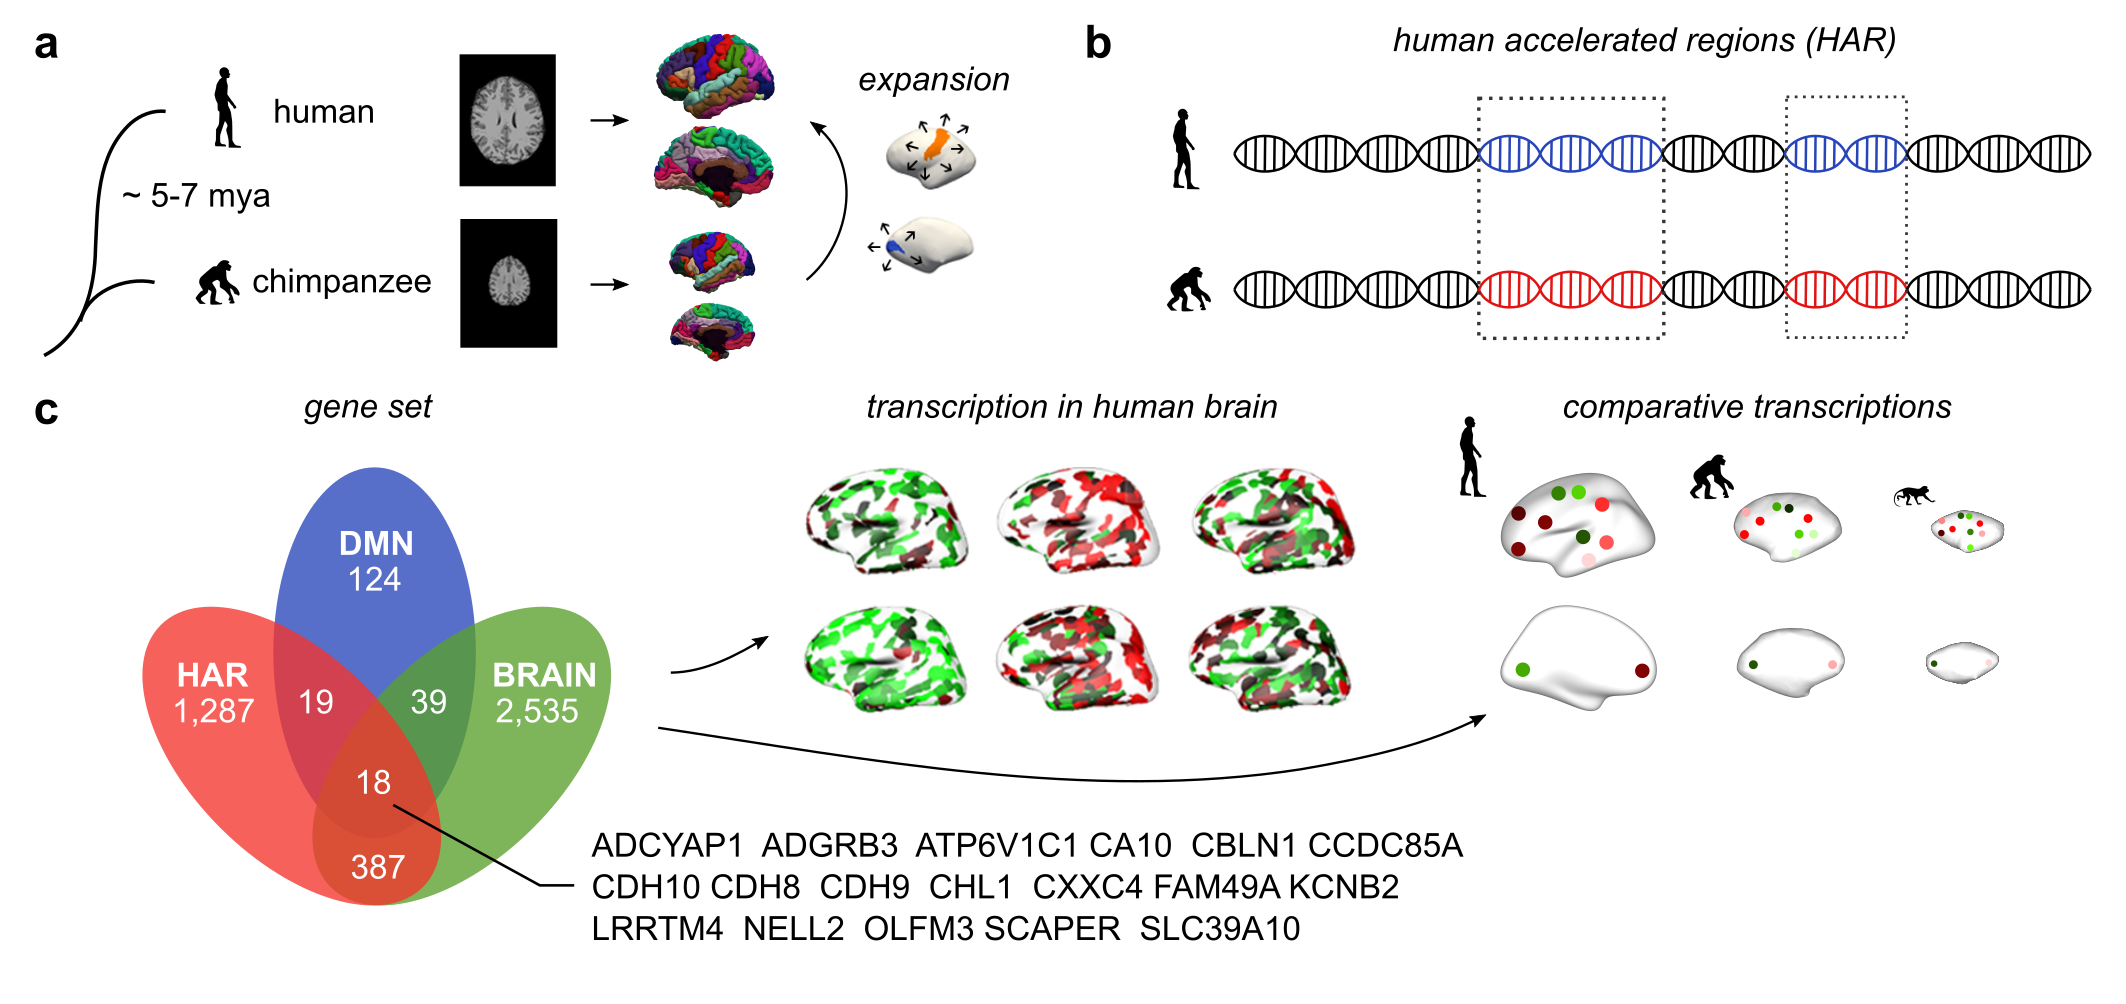
\includegraphics[width=\linewidth]{images/harFig1.png}
    \caption{Methods overview. (a) The human and chimpanzee cortex were constructed using MRI data, with chimpanzee-to-human cortical expansion computed based on the reconstructed cortical maps. (b) Genes associated with human accelerated regions (HAR), which represent genomic loci with accelerated divergence in humans, were examined. (c) Cortical gene expression of HAR genes and HAR-BRAIN genes were examined using human transcription data from the Allen Human Brain Atlas (AHBA) and comparative transcription data of the human, chimpanzee, and macaque from the PsychENCODE database.}
    \label{harFig1}
\end{figure}

\section*{Results}
\subsection*{Human cortical expansion}
We started by mapping the expansion of the human cortex (\textit{Homo sapiens}) compared to the cortex of the chimpanzee (\textit{Pan troglodytes}), one of our closest living evolutionary relatives along with the bonobo (\textit{Pan paniscus}). Cortical morphometry of the chimpanzee and human cortex was assessed using a surface-to-surface mapping of 3D reconstructions of the cortical mantle across both species, based on in vivo T1-weighted MRI (29 chimpanzees, 30 humans; Figure \ref{harFig1}a). The largest expansion of the human cortex was found in areas of bilateral orbital inferior frontal gyrus ($\times$4.0 expansion), rostral middle frontal lobe ($\times$3.8 expansion), inferior/middle temporal lobe ($\times$3.0/2.9 expansion), lingual gyrus ($\times$2.9 expansion), right inferior parietal lobe ($\times$3.7 expansion), and left precuneus ($\times$2.7 expansion; two-sample \tvaldf-test on the normalized expansion, \textit{q} < 0.001, false discovery rate [FDR] corrected; Cohens'\textit{d} > 0.989; Figure \ref{harFig2}a). The lowest expansion was found in primary areas, including bilateral precentral gyrus ($\times$1.3 expansion), postcentral gyrus ($\times$1.4 expansion), and paracentral lobe ($\times$1.2 expansion; \textit{q} < 0.001, FDR corrected; Cohens'\textit{d} < -1.047; Figure \ref{harFig2}a and Supplementary Data 1 in \citep{Wei2019GeneticMA}).

We next grouped cortical areas into the visual (VN), somatomotor (SMN), dorsal-attention (DAN), limbic (LN), ventral-attention (VAN, also commonly referred to as the salience network), frontoparietal (FPN), and default-mode network (DMN) (Figure \ref{harFig2}b and Supplementary Methods) \citep{thomas2011organization}. Higher-order cognitive networks (i.e., DMN, FPN, VAN) displayed particularly high levels of cortical expansion as compared to the SMN/VN ($\times$1.2 larger expansion in regions of higher-order cognitive networks combined compared to the regions of the SMN/VN combined, two-sample \tvaldf-test, \tvaldf(86) = 3.257, \pval = 0.002; Figure \ref{harFig2}d). FPN showed the largest expansion (mean: $\times$2.9 expansion), with the DMN in second place (mean: $\times$2.4 expansion), showing both significantly higher expansion when comparing each of them with the rest of the brain (FPN: \tvaldf(108) = 3.360, \pval = 0.001; DMN: \tvaldf(108) = 2.621, \pval = 0.010; FDR corrected; Supplementary Table \ref{table3S1}). In contrast, separately examining the other five networks did not show significant increases in the expansion of these networks compared to the rest of the cortex.

\begin{figure}[h]
    \centering
    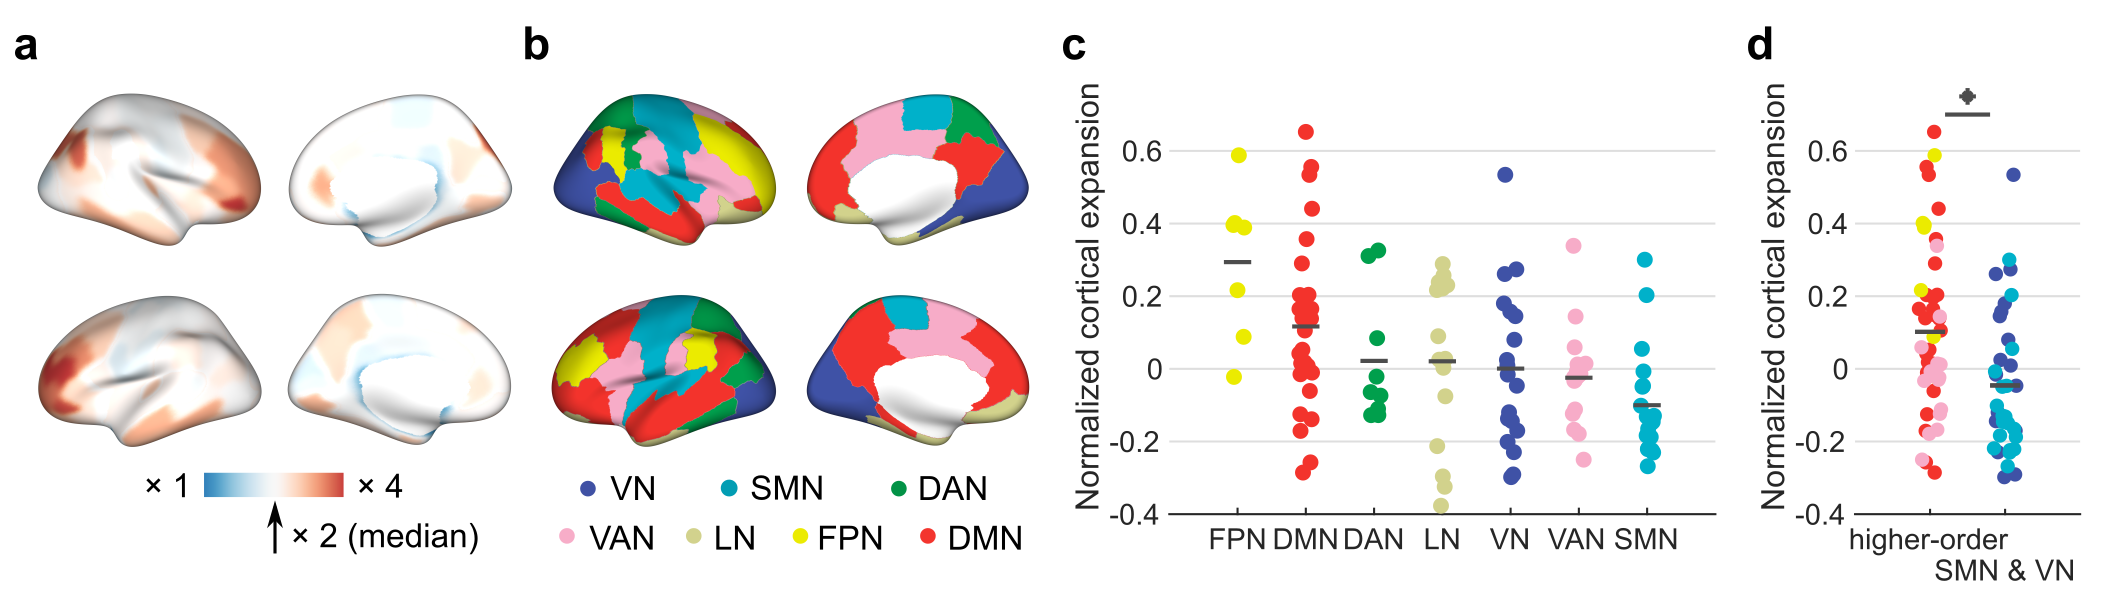
\includegraphics[width=\linewidth]{images/harFig2.png}
    \caption{Cortical expansion. (a) Cortical expansion from chimpanzees to humans. Blue: below-median human expansion (i.e., < $\times$2 expansion compared to chimpanzee); red: above-median expansion (i.e., > $\times$2). (b) Brain maps of the seven resting-state functional networks according to the DK-114 atlas, describing the visual (VN), somatomotor (SMN), dorsal-attention (DAN), limbic (LN), ventral-attention (VAN), frontal-parietal (FPN), and default-mode network (DMN). (c) Levels of normalized cortical expansion per functional network in descending order of mean expansion. (d) Levels of normalized cortical expansion in higher-order cognitive networks (DMN, FPN, VAN) versus the SMN and VN. Dots depict cortical regions. Colors represent functional networks, as in panel b. Central marks are mean expansions. * indicates a two-sided \textit{p}-value < 0.05, FDR corrected, two-sample \tvaldf-test.}
    \label{harFig2}
\end{figure}

\subsection*{HAR gene expression}
We then examined this distinct pattern of human cortical expansion across the seven resting-state functional networks in relation to cortical gene expression patterns relevant to human evolution. Microarray data on gene expression across cortical regions were obtained from the Allen Human Brain Atlas (AHBA) (\url{http://human.brain-map.org/}), containing transcriptional profiles of 20,734 genes across 57 areas of the left cortical mantle (Figure \ref{harFig1}c). Genes relevant to human evolution were taken as the list of 2143 genes associated with HAR as presented previously by Doan and colleagues \citep{doan2016mutations}, selected based on positional mapping. Alternative selection and allocation of HAR-associated genes are possible (e.g., using chromatin interactions) and we examined such alternatives to validate our results (Supplementary Note 1).

Transcription data of 1711 HAR-associated genes were present in AHBA (referred to as HAR genes; Supplementary Data 2 in \citep{Wei2019GeneticMA}), and we further examined their cortical gene expression levels in comparison to the cortical expansion. The expression profile of HAR genes was positively correlated to the pattern of human cortical expansion (Pearson's \rvaldf(53) = 0.360, \pval = 0.007; Supplementary Figure \ref{harFigs1}a), indicating the highest HAR gene expression in highly expanded areas of the human cortex. This association significantly exceeded the null condition of correlations between cortical expansion and expression of random gene sets (i.e., 1711 random genes) selected from a pool of 8686 genes related to general evolutionarily conserved genetic elements (ECE genes \citep{lindblad2011high}; \pval < 0.001, permutation test, 10,000 permutations; Supplementary Figure \ref{harFigs1}). Cortical regions of cognitive networks also showed significantly higher expression of HAR genes compared to regions of the SMN/VN (\tvaldf(44) = 2.742, \pval = 0.009; FDR corrected; Supplementary Figure \ref{harFigs1}b), with regions of the DMN showing the highest HAR gene expression (\tvaldf(55) = 2.274, \pval = 0.027, uncorrected, comparing the DMN to all other networks combined; Supplementary Figure \ref{harFigs1}c). These effects again significantly exceeded the null conditions of effects of random ECE genes (all \pval < 0.001, 10,000 permutations). Furthermore, examining the other six functional networks separately did not show a significant enhancement of HAR gene expression (see Supplementary Table \ref{table3S2}).

\subsection*{HAR-BRAIN gene expression}
With the set of HAR genes describing genes involved in all sorts of functions across the entire human body (and thus not specific to 'brain'), we continued by examining whether HAR genes related to brain processes may have played a specific role in the large cortical expansion of cognitive functional networks in human evolution. We identified genes commonly expressed in brain areas using the GTEx database (\url{https://www.gtexportal.org/}), selecting 2979 genes significantly more expressed in brain tissues compared to other available body sites (\textit{q} < 0.05, FDR corrected; one-sided two-sample t-test; referred to as BRAIN genes); 415 genes (24.3\%) out of the full set of 1711 HAR genes were observed to be significantly more expressed in brain tissues, a set from now on referred to as HAR-BRAIN genes (in contrast to HAR-nonBRAIN genes; see Supplementary Data 2 in \citep{Wei2019GeneticMA}).

We then aimed to examine (1) whether HAR-BRAIN genes were more expressed particularly in regions of higher-order cognitive networks compared to the total set of HAR genes, and (2) to what extent HAR-BRAIN genes were more expressed in regions of higher-order cognitive networks, more than an average set of genes related to general brain processes (i.e., BRAIN genes). First, the cortical expression pattern of HAR-BRAIN genes was significantly correlated with the pattern of human cortical expansion (\rvaldf(53) = 0.488, \pval < 0.001; Figure \ref{harFig3}c). Furthermore, HAR-BRAIN genes showed significantly higher expression in regions of cognitive networks as compared to the SMN/VN (\tvaldf(44) = 5.136, \pval < 0.001, FDR corrected; Figure \ref{harFig4}a), with the highest expression levels again observed in the DMN (\tvaldf(55) = 3.267, \pval = 0.002, FDR corrected, DMN versus the rest of the cortex; Figure \ref{harFig4}b). These effects were, respectively, $\times$3.2 and $\times$2.7 larger than the effect obtained by HAR-nonBRAIN genes (\tval(55) = 1.028, \pval = 0.309 and \tvaldf(55) = 1.212, \pval = 0.232, separately, Supplementary Figure \ref{harFigs2}). Notably, examining the other six functional networks separately did not show any significant elevations of HAR-BRAIN gene expression (Supplementary Table \ref{table3S3}), suggesting the highest expression level in the DMN.

\begin{figure}[h]
    \centering
    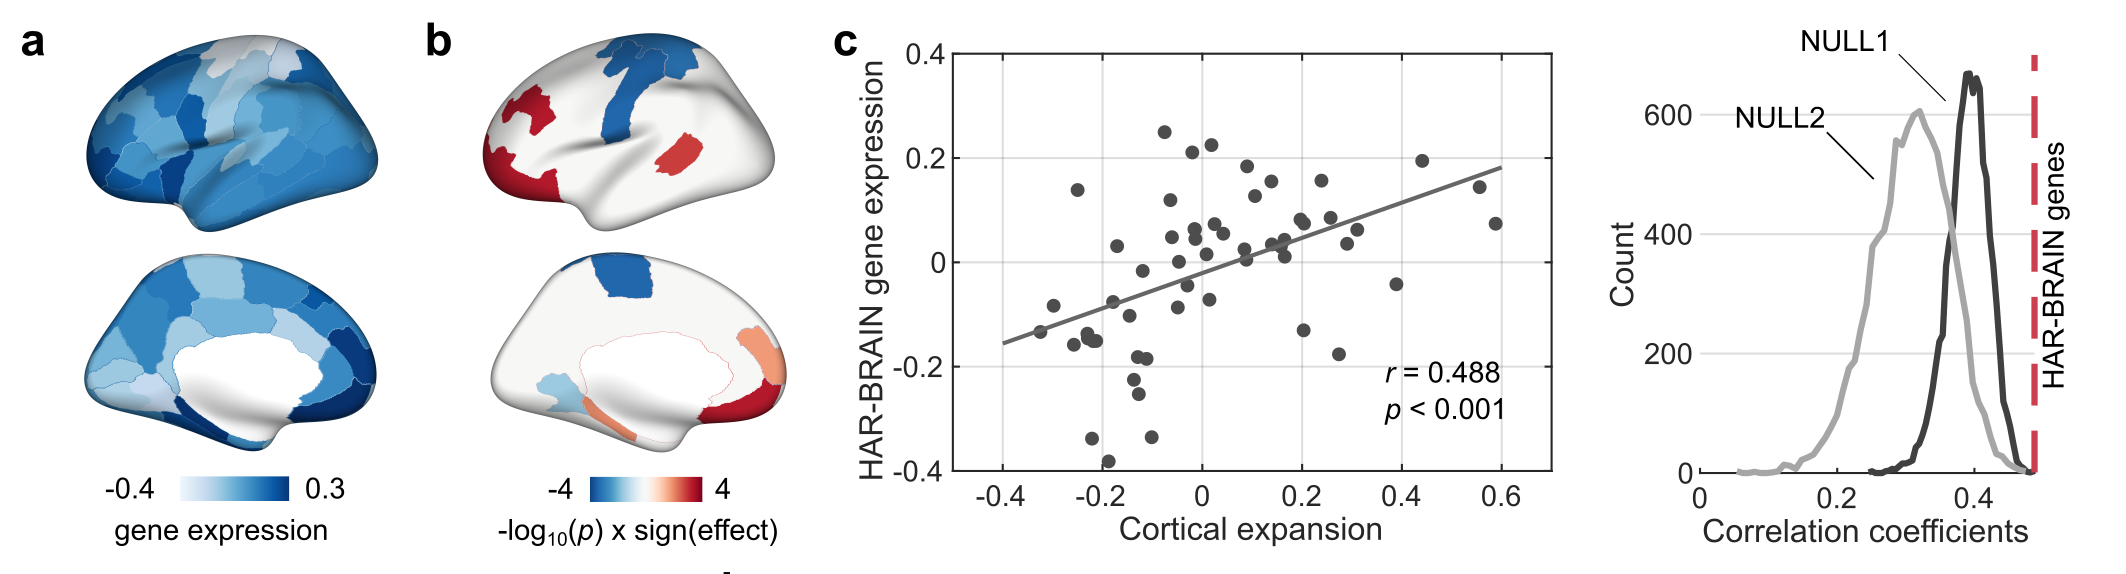
\includegraphics[width=\linewidth]{images/harFig3.png}
    \caption{HAR-BRAIN gene expression. (a) Cortical gene expression of HAR-BRAIN genes. (b) Cortical maps of the significance level obtained by permutation tests, comparing expressions of HAR-BRAIN genes to equally sized random gene-sets taken from BRAIN (NULL1) and ECE genes (NULL2). (c) Association between the gene expression profile of HAR-BRAIN genes and normalized cortical expansion between human and chimpanzee (left). The correlation coefficient is significantly higher than NULL1 and NULL2 (both \pval < 0.001, two-sided, permutation test; right).}
    \label{harFig3}
\end{figure}

Second, we compared HAR-BRAIN gene expression with two types of null distributions of expression differences generated by randomly selecting the same number of genes (i.e., 415) from the pool of 2979 BRAIN genes (referred to as NULL1) and 8686 ECE genes (referred to as NULL2). The elevated expression of HAR-BRAIN genes in regions of higher-order cognitive networks was significantly larger than both null distributions (\pval = 0.006 and \pval < 0.001 for NULL1 and NULL2, respectively; 10,000 permutations; Figure \ref{harFig4}b). The same result was observed when examining DMN regions specifically (\pval < 0.001 for both NULL1 and NULL2; 10,000 permutations; Figure \ref{harFig4}c), suggesting a specific role of HAR-BRAIN genes in differentiating DMN regions from the rest of the brain. Permutation testing based on randomly shuffling cortical areas showed similar results (Supplementary Figure \ref{harFigs3}). An exploratory examination on gene expression in each individual further demonstrated that the differentiation of HAR-BRAIN gene expression between the DMN and the rest of the cortex significantly correlated with the ratio of brain volume of the DMN regions (\rvaldf(4) = 0.839, \pval = 0.037; Supplementary Figure \ref{harFigs4}).

\begin{figure}[h]
    \centering
    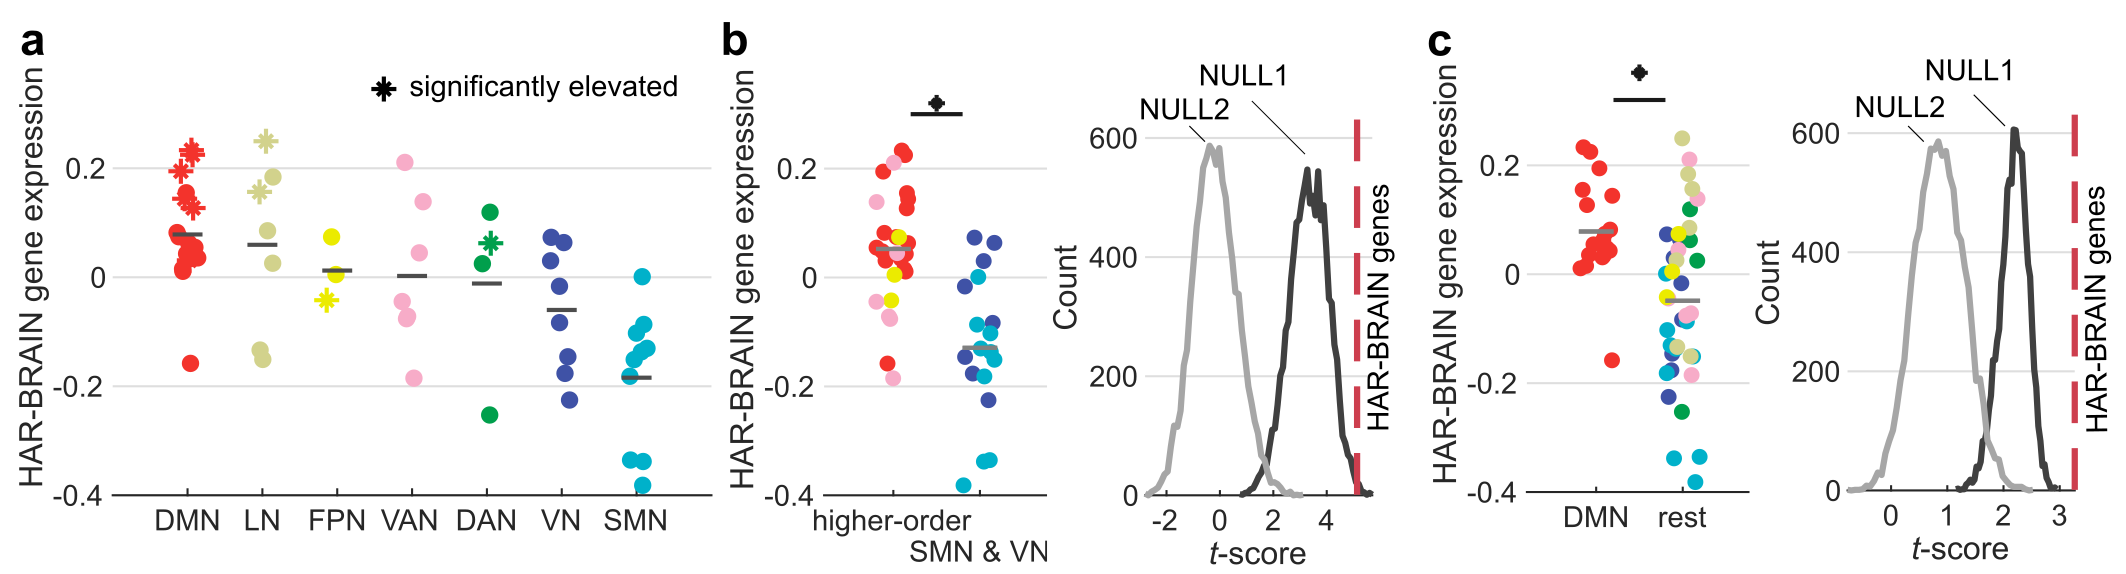
\includegraphics[width=\linewidth]{images/harFig4.png}
    \caption{HAR-BRAIN genes expression across functional networks. (a) HAR-BRAIN gene expression within each of the seven functional networks ranked in descending order of the mean expression. Asterisks (*) indicates significantly upregulated regions as in Figure \ref{harFig3}. (b) HAR-BRAIN gene expression in cognitive networks (DMN, FPN, and VAN) versus the SMN and VN (left), with permutation results demonstrated in the right panel (two-sided \pval = 0.003 and \pval < 0.001 for NULL1 and NULL2, respectively). (c) HAR-BRAIN gene expression in the DMN versus the rest of the cortex (left), with permutation results demonstrated in the right panel (two-sided \pval < 0.001 for both NULL1 and NULL2).}
    \label{harFig4}
\end{figure}

We then examined HAR-BRAIN expression for each of the cortical regions of the 7 functional networks separately; 10 cortical areas showed significantly high expression of HAR-BRAIN genes compared to a random selection of genes out of both BRAIN (NULL1) and ECE genes (NULL2) (FDR corrected, \textit{q} < 0.05; 10,000 permutations; Figure \ref{harFig3}b). Importantly, 7 out of these 10 regions described regions of the higher cognitive networks and 6 out of these 7 regions described DMN regions (\pval = 0.034 and 0.008, respectively; hypergeometric test). These findings together suggest a specific role of HAR-BRAIN genes in the architecture of cognitive functional brain networks, beyond effects of general evolutionary conserved genes and general BRAIN genes.

\subsection*{Chimpanzee-human comparative gene expression}
Our analyses so far suggested that HAR-BRAIN genes were more expressed in highly expanded regions of higher-order cognitive networks, but did not yet provide direct information on whether HAR-BRAIN gene expression is upregulated in the human brain compared to that of other primate species. To examine this, we used gene expression data from the PsychENCODE database (\url{http://evolution.psychencode.org/}) \citep{sousa2017molecular}, which describes gene expression of 11 comparable cortical regions across the human, chimpanzee, and macaque. Due to the lower spatial sampling of cortical regions (data of 3 DMN regions available, Figure \ref{harFig5}a), we limited our examination to a comparison between cognitive networks and the SMN/VN. First, we replicated the observation of high expression of HAR-BRAIN genes in regions of higher-order cognitive networks compared to regions of the SMN/VN in humans (\tvaldf(8) = 7.135, \pval < 0.001; Figure \ref{harFig5}b), with this effect significantly exceeding both NULL1 and NULL2 (both \pval < 0.001, 10,000 permutations). This confirmed our AHBA-based findings of high HAR-BRAIN gene expression in cognitive networks in the human brain. Second, the differentiating level of HAR-BRAIN gene expression between cognitive and primary areas observed in humans (Cohen's \textit{d} = 4.605) was found to be $\times$2.7 larger than the effects found in chimpanzees (Cohen's \textit{d} = 1.695) and $\times$2.8 larger compared to macaques (Cohen's \textit{d} = 1.616). Chimpanzees and macaques showed only marginally higher HAR-BRAIN gene expression in regions of higher-order cognitive networks as compared to the SMN/VN (chimpanzees: \tvaldf(8) = 2.626, \pval = 0.030; macaques: \tvaldf(8) = 2.504, \pval = 0.037). Furthermore, the difference in effect size between humans and chimpanzees was larger than expected based on NULL1 and NULL2 (both \pval < 0.001; human-macaque: NULL1, \pval = 0.026 and NULL 2, \pval = 0.090, only trend-level, not significant [n.s.]; 10,000 permutations; Supplementary Figure \ref{harFigs5}).

\begin{figure}[h]
    \centering
    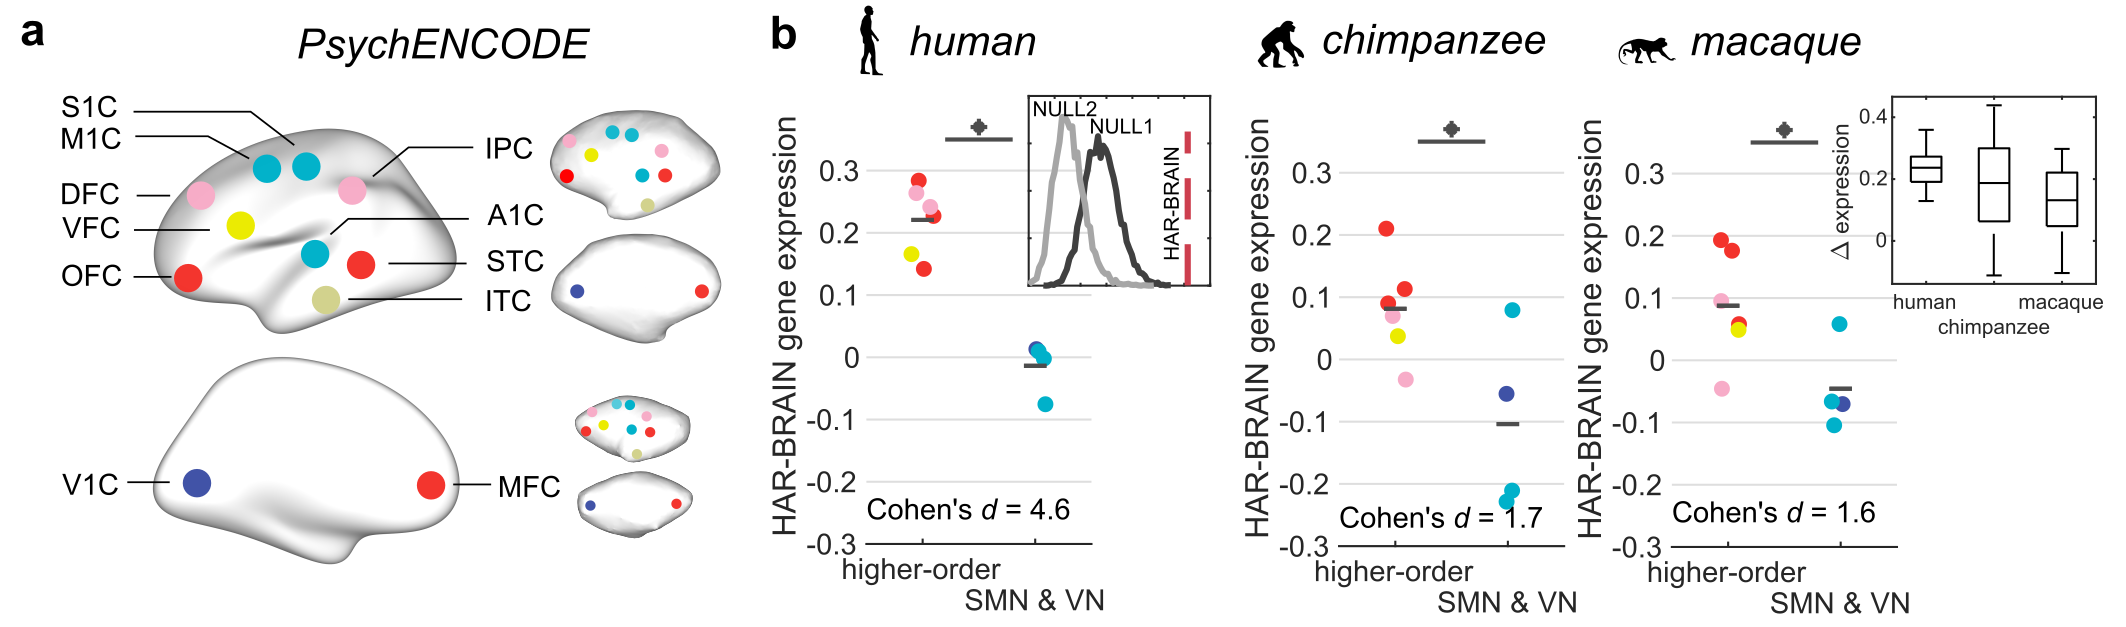
\includegraphics[width=\linewidth]{images/harFig5.png}
    \caption{HAR-BRAIN genes expression in human, chimpanzee, and macaque. (a) Species-homologous brain areas as presented in the PsychENCODE dataset for the human (left), chimpanzee (upper right), and macaque (lower right). (b) Normalized expression levels of HAR-BRAIN genes in regions of higher-order networks compared to areas of the SMN/VN in humans (\pval < 0.001, two-sample \tval test). Largest differences in gene expression are found in humans, with chimpanzees in second place, followed by macaques (\pval = 0.002, Jonckheere-Terpstra test). Asterisks (*) indicates two-sided \pval < 0.05, FDR corrected. Central marks denote the mean gene expression. Boxplot center, median; box = 1st-3rd quartiles (Q); lower whisker, Q1 - 1.5 $\times$ interquartile range (IQR); upper whisker, Q3 + 1.5 $\times$ IQR. Colors indicate the assignment of functional networks, as in Figure \ref{harFig2}b. M1C primary motor cortex, S1C primary sensory cortex, IPC inferior parietal cortex, STC superior temporal cortex, ITC inferior temporal cortex, A1C primary auditory cortex, OFC orbital frontal cortex, VFC ventral frontal cortex, DFC dorsal frontal cortex, V1C primary visual cortex, MFC medial frontal cortex.}
    \label{harFig5}
\end{figure}


Further evaluation of this cross-species effect showed a significantly decreasing step-wise relationship of differences in HAR-BRAIN gene expression between regions of higher-order networks and the SMN/VN from humans (highest) to chimpanzees and macaques (lowest differentiating expression, Jonckheere-Terpstra test, \pval = 0.002). To reduce the influence of a relatively large variance of expression levels within chimpanzees and macaques (Figure \ref{harFig5}b), we performed a leave-one-out analysis (iteratively leaving out one region at a time) and confirmed a larger mean gene expression difference between cognitive network regions and primary regions in humans in comparison to chimpanzees and macaques (Supplementary Figure \ref{harFigs6}). These findings thus suggest that humans display upregulated expression of HAR-BRAIN genes in brain areas involved in cognitive brain function as compared to other primates.

\subsection*{Top strongest differentiating DMN genes}
We continued by investigating the biological properties of genes showing the highest levels of expression in DMN regions out of all genes. For each gene in AHBA, we computed the upregulated level of gene expression in regions of the DMN by calculating the \tvaldf-score for expressions of the selected gene in regions of the DMN against the rest of the brain. The top 200 highly expressed genes (i.e., genes showing the highest positive \tvaldf-scores, referred to as DMN genes; all \pval < 0.004) were taken as the DMN’s most differentiating genes (see Supplementary Data 3 in \citep{Wei2019GeneticMA}). Out of the top 200 DMN genes, we identified 37 to be HAR genes, particularly including 18 HAR-BRAIN genes, which greatly exceeded the chance level of randomly selecting 37 or 18 out of 20,734 genes (both \pval < 0.001, hypergeometric test). We also examined the top 53 genes with \pval < 0.0014 (partial Bonferroni corrected, see Supplementary Methods) and top 469 genes with \pval < 0.01 (uncorrected), which revealed comparable findings (Supplementary Note 2).

To investigate whether the observed effect was restricted to the DMN, an additional permutation analysis was performed by shuffling region labels and re-computing the top genes for each of these random network assignments. We found the ratio of HAR genes in the set of top DMN genes to be significantly higher than the null condition (\pval < 0.001, 10,000 permutations), which confirmed a dominant role of HAR genes in DMN organization. To further examine potential DMN specificity, we also selected the top 200 genes showing the largest differentiating gene expression in each of the other functional networks compared to the SMN/VN. In contrast to the DMN (revealing 18 overlapping genes with the set of HAR-BRAIN genes), the top 200 gene sets identified by the VAN, DAN, FPN, and LN, comprised, respectively, only 12,8,7 and 7 HAR-BRAIN genes.

Gene-set enrichment analysis on the set of DMN genes using hypergeometric testing in the web-based platform FUMA \citep{watanabe2017functional} showed significant over-representation of DMN genes in Gene Ontology (GO) terms related to cellular components of dendrite (\pval = 2.60 $\times$ 10\textsuperscript{-5}), somatodendritic compartment (\pval = 4.49 $\times$ 10\textsuperscript{-5}), synapse (\pval = 2.15 $\times$ 10\textsuperscript{-4}), perikaryon (\pval = 7.45 $\times$ 10\textsuperscript{-5}) and neuron projection terminus (\pval = 2.26 $\times$ 10\textsuperscript{-4}), as well as molecular functions of neuropeptide hormone activity and calcium activated potassium/cation channel activity (\pval = 1.66 $\times$ 10\textsuperscript{-5} and 1.32 $\times$ 10\textsuperscript{-4}; FDR corrected; Supplementary Table \ref{table3S4}).

\subsection*{GWAS on DMN functional activity}
We then wanted to examine whether HAR/HAR-BRAIN genes played a role in inter-subject variation in default-mode functional activity in today's human population. We performed a GWAS on 6,899 participants from the UK Biobank \citep{sudlow2015uk} (see Supplementary Methods) with the amplitude of fMRI time series of the independent component analysis (ICA)-based resting-state networks ("NETMAT amplitudes 25"\citep{elliott2018genome} as described in \url{https://www.fmrib.ox.ac.uk/ukbiobank/}) as the phenotypes of interest. Particularly, we focused on the amplitude of the ICA component No.1 that resembles the DMN (referred to as DMN amplitude, Figure \ref{harFig6}a). GWAS results for all single-nucleotide polymorphisms (SNP) with minor allele frequency (MAF) > 0.005 were assessed (Figure \ref{harFig6}b). The quantile-quantile plot showed a linkage disequilibrium score regression [LDSC] intercept of 0.999 (standard error [s.e.] = 0.006), with an inflation level of \textlambda\textsubscript{GC} = 1.005 and mean \textchi\textsuperscript{2} statistic = 1.012. LDSC-based SNP heritability [\textit{h}\textsuperscript{2}\textsubscript{SNP}] was 0.09 [s.e. = 0.06]. We observed 3 independent (\textit{r}\textsuperscript{2} < 0.1) genome-wide significant SNPs (\pval < 5 $\times$ 10\textsuperscript{-8}; using linear regression model; Figure \ref{harFig6}b) across 2 genomic loci (Figure \ref{harFig6}c). Furthermore, we annotated 19 significant SNPs (\pval < 5 $\times$ 10\textsuperscript{-8}) with high LD (\textit{r}\textsuperscript{2} $\geq$ 0.6) to the 3 independent SNPs using gene-mapping functions in FUMA \citep{watanabe2017functional} (see Methods section), which resulted in a set of 12 genes (Supplementary Table \ref{table3S5}; three genes [\textit{PLCE1}, \textit{NOC3L}, and \textit{SLC35G1}] annotated using brain-related eQTL and Hi-C mappings). Hypergeometric testing \citep{watanabe2017functional} showed significant enrichment of the 12 genes in the GWAS catalog \citep{buniello2018nhgri} reported gene-set "plasma clozapine-norclozapine ratio in treatment-resistant schizophrenia" (\pval = 1.26 $\times$ 10\textsuperscript{-12}; Supplementary Table \ref{table3S6}). None of the genes overlapped with HAR-BRAIN genes or the top 200 DMN. One gene (\textit{INPP5A}) denoted as a HAR gene.

We further investigated the potential association of HAR/HAR-BRAIN genes with variations in DMN amplitude using MAGMA linear-regression-based gene-set analysis\citep{de2015magma}. We found HAR-BRAIN genes to be significantly associated with the phenotypic variation in DMN amplitude (\textbeta \ = 0.015, \pval  = 0.016, FDR corrected). No significant effect was found for the set of HAR genes (\textbeta \ = 0.011, \pval = 0.051; Supplementary Table \ref{table3S7}) or DMN genes (\textbeta \ = 0.005, \pval = 0.219). An additional conditional gene-set analysis \citep{de2018conditional} including the set of BRAIN genes as a covariate, further showed a significant association of HAR-BRAIN genes with variations in DMN amplitude (\textbeta \ = 0.014, \pval = 0.022; HAR genes: \textbeta \ = 0.011, \pval = 0.055; Figure \ref{harFig6}e). Furthermore, no significant effect was observed when we examined the association between HAR-BRAIN genes and amplitude of other ICA components resembling the rest of the functional networks (\pval > 0.09; Figure \ref{harFig6}f and Supplementary Table \ref{table3S8}), implicating a specific role of HAR-BRAIN genes in genetic variations of DMN functional activity. Using the normalized DMN amplitude (corrected for the mean amplitude across all networks) as the phenotype of interest showed similar results (HAR genes: \textbeta \ = 0.018, \pval = 0.003; HAR-BRAIN genes: \textbeta \ = 0.020, \pval = 0.002; Supplementary Figure \ref{harFig7}).

Stratified LDSC analysis \citep{finucane2015partitioning} did not result in findings of significant enrichment of genetic variance of DMN functional activity explained by SNPs overlapping with HAR regions. This is likely related to HARs occupying relatively small regions in the whole genome with a mean length of only 256 base pairs (Supplementary Figure \ref{harFigs8}), which limits statistical power to perform such post-hoc analyses. The relatively large s.e. of the SNP heritability might be related to the limited sample size.

\begin{figure}[H]
    \centering
    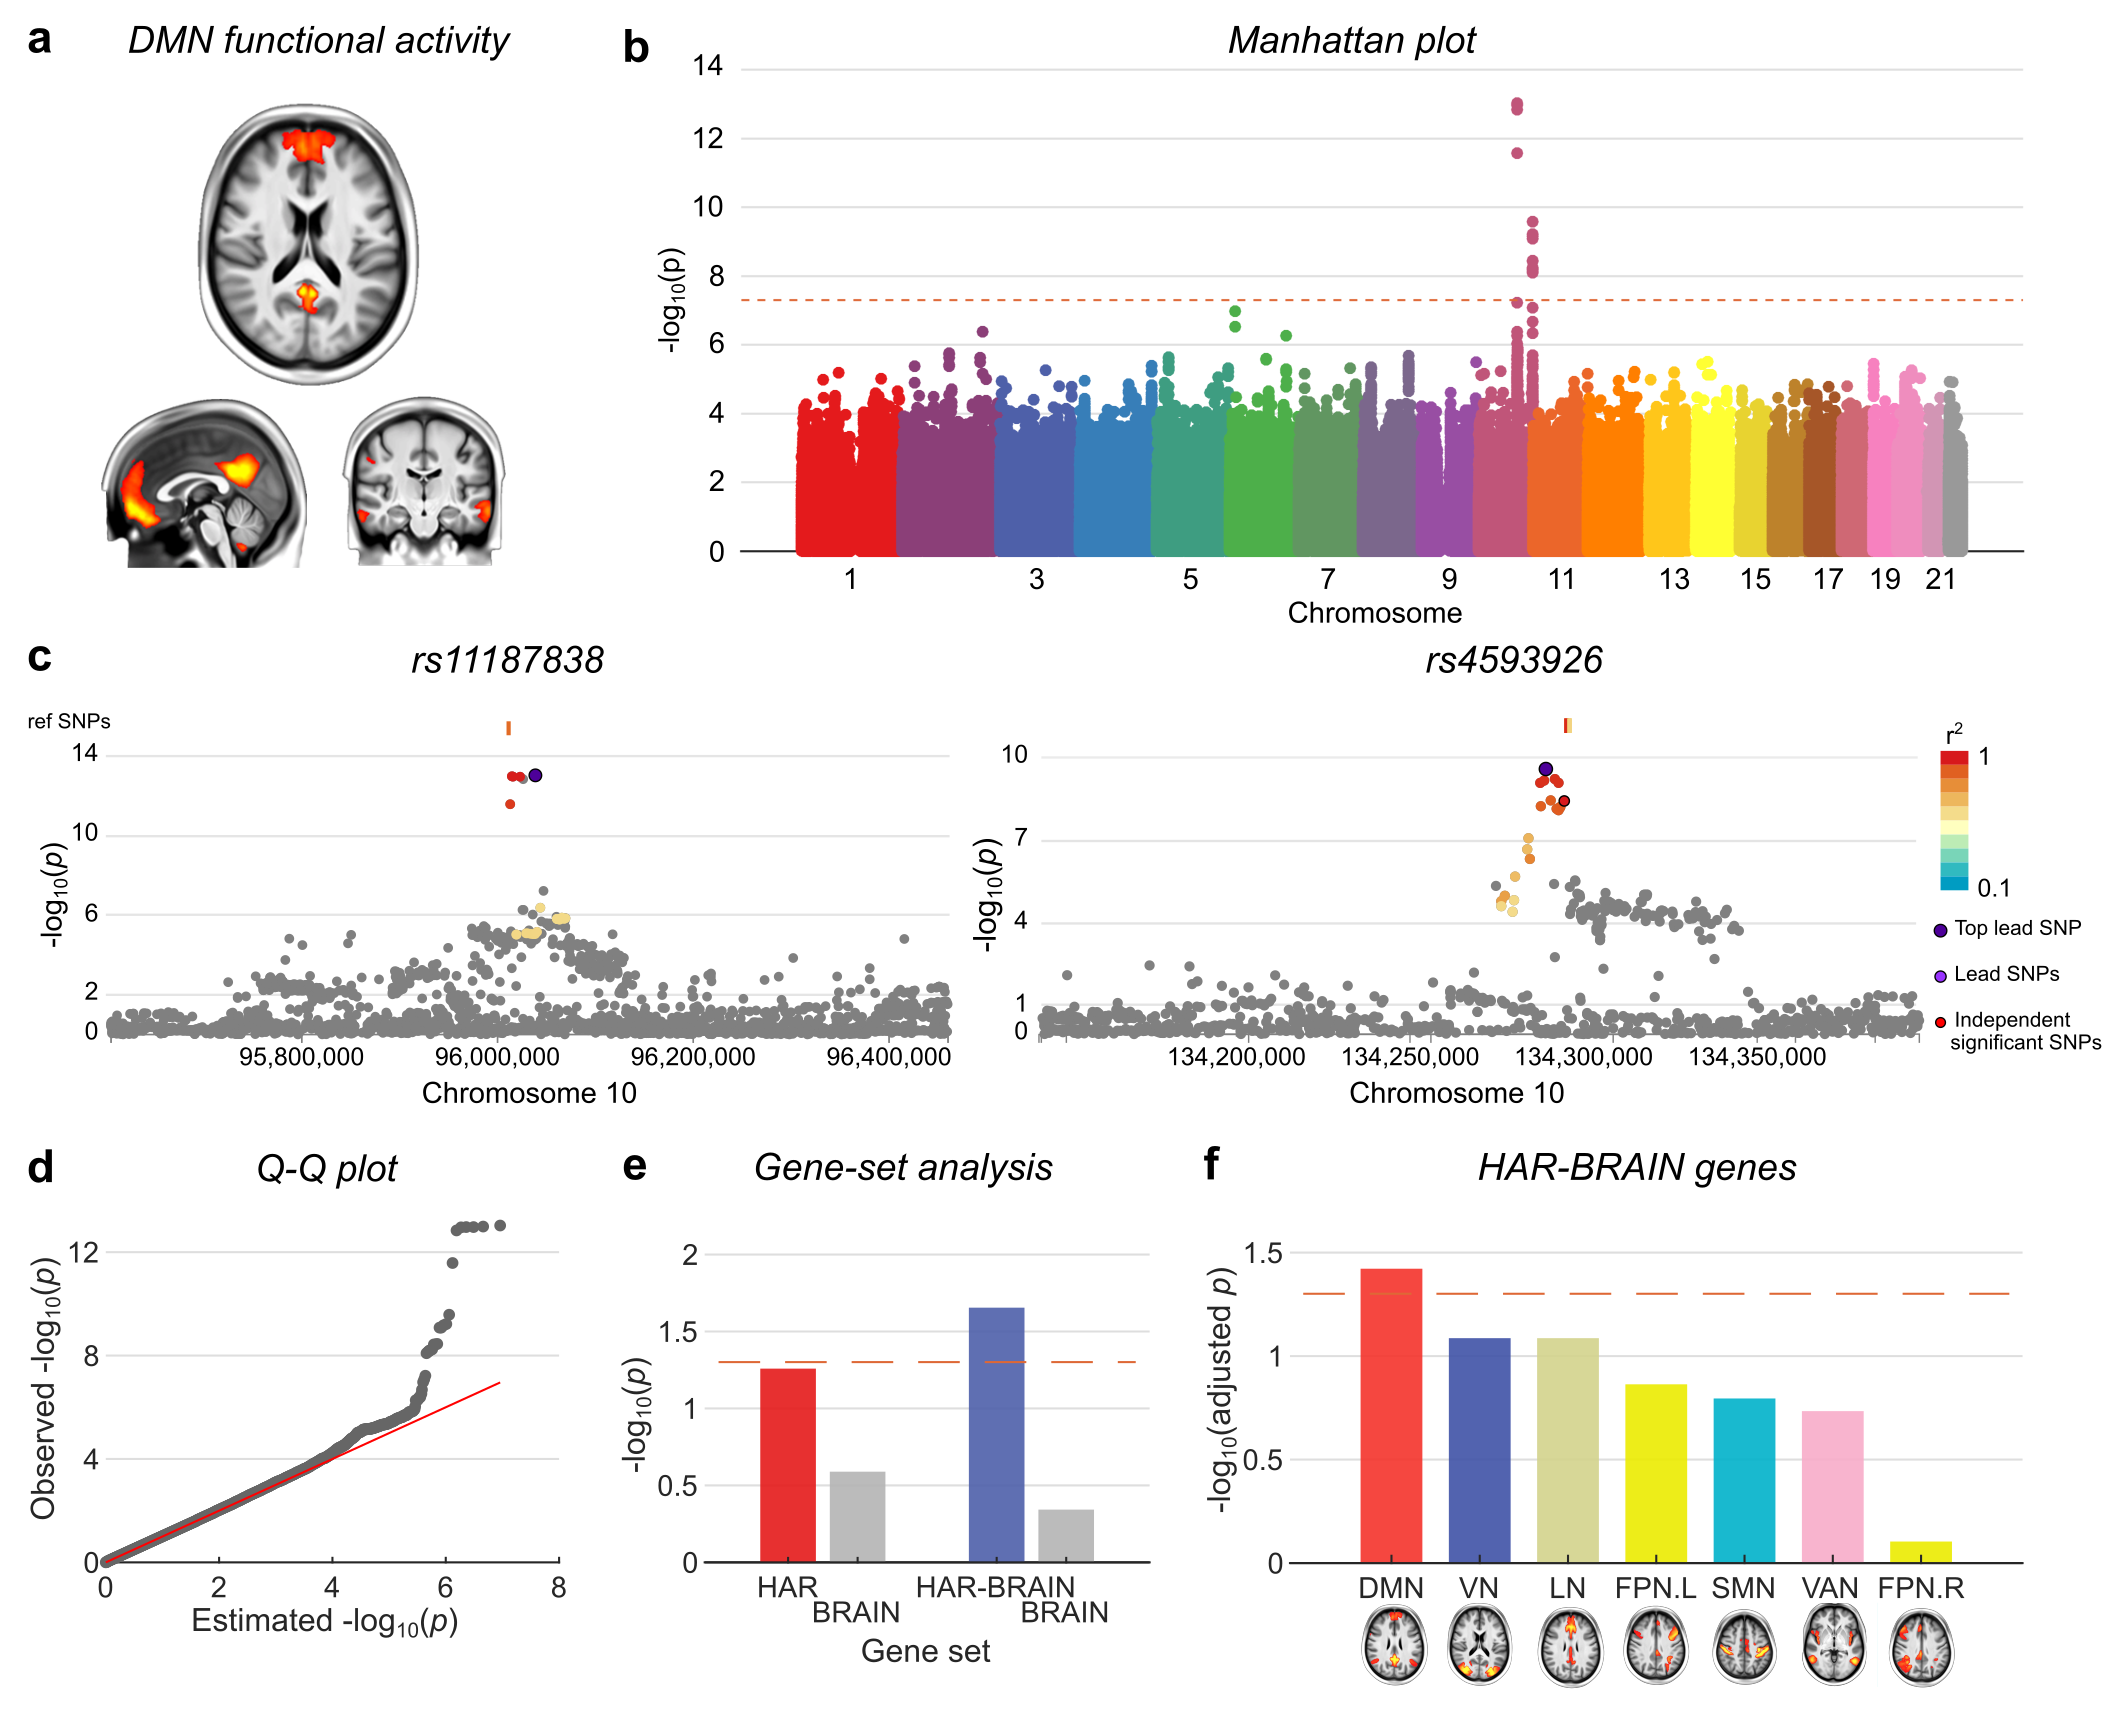
\includegraphics[width=\linewidth]{images/harFig6.png}
    \caption{GWAS on DMN activity. (a) DMN component. (b) GWAS Manhattan plot showing -log10-transformed two-tailed \textit{p}-value for all SNP (y-axis) and base-pair positions along the chromosomes (x-axis). Dotted red line indicates Bonferroni-corrected genome-wide significance (\textit{p}-value < 5 $\times$ 10\textsuperscript{-8}). (c) Regional plots of the two genomic loci (left, lead SNP: rs11187838 and right, lead SNP: rs4593926). (d) Q-Q plot of SNP-based \textit{p}-value in panel (b). Observed -log10 transformed two-tailed \textit{p}-values of associations with DMN functional activity are plotted against expected null \textit{p}-values for all SNPs in the GWAS. (e) MAGMA conditional gene-set analysis. -log10-transformed \textit{p}-values of the associations between HAR/HAR-BRAIN genes and DMN functional activity conditional upon BRAIN genes. Dashed line indicates \pval = 0.05. (f) MAGMA gene-set analysis on HAR-BRAIN genes and other "NETMAT amplitude 25" phenotypes representing functional activity in the other functional networks (-log10-transformed adjusted \textit{p}-values, FDR corrected). Colors indicate the assignment of functional networks, as in Figure \ref{harFig2}b. Dashed line indicates adjusted \pval = 0.05.}
    \label{harFig6}
\end{figure}

\subsection*{HAR genes, cognitive abilities, and psychiatric disorders}

We then examined the potential role of HAR/HAR-BRAIN and DMN genes in human cognition by cross-referencing these genes with a recent GWAS meta-analysis on intelligence (\textit{h}\textsuperscript{2}\textsubscript{SNP} = 0.184 [s.e. = 0.008]) performed on 269,867 individuals \citep{Savage2018GenomewideAM}. Gene-set analysis \citep{de2015magma} revealed both sets of HAR and HAR-BRAIN genes to be significantly associated with individual variations in intelligence (HAR: \textbeta\ = 0.058, \pval = 5.43 $\times$ 10\textsuperscript{-10}; HAR-BRAIN: \textbeta\ = 0.075, \pval = 1.22 $\times$ 10\textsuperscript{-15}; Supplementary Table \ref{table3S7}). Conditional gene-set analysis \citep{de2018conditional} including BRAIN genes as a covariate further confirmed a significant association of both HAR and HAR-BRAIN genes with intelligence (HAR: \textbeta\ = 0.056, \pval = 1.60 $\times$ 10\textsuperscript{-9}; HAR-BRAIN: \textbeta\ = 0.060, \pval = 6.34 $\times$ 10\textsuperscript{-10}). Intelligence was not found to be specifically associated with the total set of DMN genes (\textbeta\ = 0.012, \pval = 0.061), but a significant effect was observed for the subset of 37 intersected HAR-DMN genes (\textbeta\ = 0.022, \pval = 0.009, FDR corrected).

We next linked HAR/HAR-BRAIN and DMN genes to genetic effects on social behavior, which is thought to be more advanced in humans than in other primate species \citep{tomasello2010ape}. Summary statistics of the trait “Frequency of friend/family visits” (\textit{h}\textsuperscript{2}\textsubscript{SNP} = 0.035 [s.e. = 0.002]) based on a GWAS analysis on 383,941 individuals in the UK Biobank were obtained from the GWAS ATLAS web tool \citep{Watanabe2019AGO} (\url{http://atlas.ctglab.nl}, ID 3216). HAR/HAR-BRAIN genes were found to be significantly associated with this trait (HAR: \textbeta\ = 0.037, \pval = 1.24 $\times$ 10\textsuperscript{-7}; HAR-BRAIN: \textbeta\ = 0.039, \pval = 1.01 $\times$ 10\textsuperscript{-7}; Supplementary Table \ref{table3S7}), with effects unrelated to the set of BRAIN genes (HAR: \textbeta\ = 0.037, \pval = 1.73 $\times$ 10\textsuperscript{-7}; HAR-BRAIN: \textbeta\ = 0.036, \pval = 2.63 $\times$ 10\textsuperscript{-6}). Furthermore, DMN genes were also significantly associated with individual variation in sociability (\textbeta\ = 0.012, \pval = 0.024; HAR-DMN genes: \textbeta\ = 0.014, \pval = 0.022, FDR corrected).

We also examined the potential association of HAR/HAR-BRAIN and DMN genes with schizophrenia, a disorder hypothesized to relate to human brain evolution \citep{crow1997schizophrenia,Heuvel2019EvolutionaryMI}. We used the summary statistics of a GWAS in 33,426 schizophrenia patients and 54,065 healthy controls (\textit{h}\textsuperscript{2}\textsubscript{SNP} = 0.187 [0.008]) provided by the Psychiatric Genomics Consortium (\url{http://www.med.unc.edu/pgc/}). We observed HAR/HAR-BRAIN genes to be significantly associated with genetic variants in schizophrenia (HAR: \textbeta\ = 0.019, \pval = 0.013; HAR-BRAIN: \textbeta\ = 0.043, \pval = 5.06 $\times$ 10\textsuperscript{-7}; Supplementary Table \ref{table3S7}). These results remained significant in the conditional gene-set analysis with BRAIN genes taken as a covariate (HAR: \textbeta\ = 0.017, \pval = 0.023; HAR-BRAIN: \textbeta = 0.028, \pval = 0.001). DMN genes were not found to be significantly associated with schizophrenia (\textbeta\ = 0.011, \pval = 0.067; HAR-DMN genes: \textbeta\ = 0.005, \pval = 0.261). In addition to common variations indicated by GWAS, we further examined the enrichment of HAR/HAR-BRAIN and DMN genes in rare variants of brain disorders using the NPdenovo database (\url{http://www.wzgenomics.cn/NPdenovo/}) \citep{li2016genes}. Hypergeometric testing showed HAR and HAR-BRAIN genes to be significantly enriched in risk genes of ASD (\pval  < 0.001 and \pval = 0.005, separately) and schizophrenia (\pval < 0.001 and \pval = 0.008, separately; FDR corrected). DMN genes also showed significant enrichment in risk genes of ASD (\pval = 0.004), but not schizophrenia (\pval = 0.264; Supplementary Figure \ref{harFigs9}).

We also examined a potential association of HAR-BRAIN genes with brain changes related to psychiatric disorders. We used data from voxel-based morphometry (VBM) studies in five psychiatric brain disorders (schizophrenia, bipolar disorder, ASD, major depressive disorder [MDD] and obsessive-compulsive disorder [OCD]) and created a cortical map describing the distribution of cortical volume changes of these five psychiatric disorders (including in total of 260 VBM studies). The spatial pattern of disorder involvement across the cortex was significantly associated with the gene expression pattern of HAR-BRAIN genes (\rvaldf(55) = 0.437, \pval < 0.001, with the cortical volume controlled; Figure \ref{harFig7}; \rvaldf(55) = 0.221, \pval = 0.098 for HAR genes), an effect significantly exceeding the effect obtained by BRAIN genes (\pval = 0.022) and ECE genes (\pval < 0.001, 10,000 permutations). For an out-group analysis, the cortical pattern of HAR-BRAIN gene expression did not correlate to the disease map of five alternative, non-psychiatric disorders (amyotrophic lateral sclerosis, stroke, alcoholism, insomnia, fibromyalgia; \rvaldf = 0.141, \pval = 0.302).

\begin{figure}[h]
    \centering
    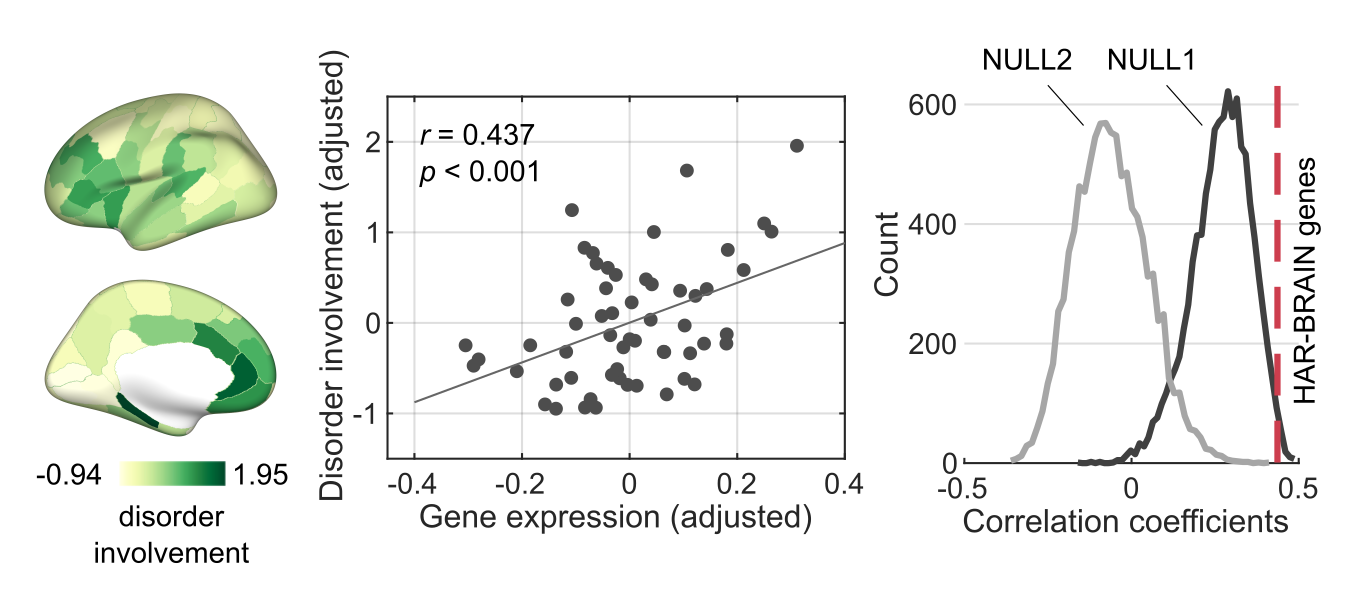
\includegraphics[width=\linewidth]{images/harFig7.png}
    \caption{Cortical disorder involvement and HAR-BRAIN gene expression. Left panel shows brain maps of cortical involvement across five major psychiatric disorders (e.g., schizophrenia, bipolar disorder, autism spectrum disorder, major depression, and obsessive-compulsive disorder). Middle panel shows correlation between HAR-BRAIN gene expression and disorder involvement (Pearson's \rvaldf(55) = 0.437, \pval < 0.001; corrected for cortical volume), and right panel shows the comparison of the correlation coefficient to null distributions generated by random BRAIN (NULL1; \pval = 0.022) and ECE genes (NULL2; \pval < 0.001, permutation test, 10,000 permutations).}
    \label{harFig7}
\end{figure}

\section*{Discussion}
Our combined comparative neuroimaging and genetic findings provide evidence of evolutionary changes in the human genome to have played a central function in the expansion and cortical organization of cognitive functional networks in the human brain, potentially in service of specialization of higher-order cognitive function in human evolution.

Our results show high levels of cortical expansion in regions of both the FPN and DMN in humans. This is compatible with prior observations of cortical expansion between macaque and human \citep{hill2010similar}, showing large expansion of associative prefrontal, temporal, and parietal areas in the human brain \citep{hill2010similar,donahue2018quantitative}. This evolutionary expansion pattern has been suggested to overlap with the pattern of cortical variation in today’s human population \citep{reardon2018normative}, suggesting larger brains to display relatively larger multi-modal associative areas, variation further linked to inter-subject variation in cognitive abilities \citep{Ryu256313}. Our observations of high expression of HAR genes in these brain areas now suggest that genes linked to hominization may have had a special role in the process of cortical development of these multimodal association areas.

Our comparative analyses further show that genes associated with human brain evolution (HAR-BRAIN genes) are not equally expressed in all cortical areas but rather are more expressed in areas related to higher-order cognitive processing. HAR genes, representing conserved loci with elevated divergence in humans \citep{pollard2006rna,doan2016mutations}, have been argued to function as important neuronal enhancers \citep{Ryu256313} and to be key players in biological processes of nervous system development and neurogenesis, amongst others (Supplementary Table \ref{table3S9}). HAR genes are enriched in human-evolved elements that converge on specific cell types and laminae involved in brain development and cerebral cortical expansion in the primate lineage \citep{won2019human} and are suggested to be particularly expressed in supragranular cortical layers important for forming cortico-cortical connectivity \citep{won2019human}. Our findings of high expression of HAR genes in central cognitive networks, and most pronounced in the DMN, may thus reflect enhanced complexity of cognitive cortical areas and circuits in human brain evolution \citep{elston2001pyramidal,jacobs2001regional}.

Our results corroborate previous observations of a strong link between aspects of cellular and macroscale connectivity \citep{vandenheuvel2019multi,scholtens2014linking}. Association areas show transcriptional profiles enriched for genes specific to the organization of supragranular layers \citep{vertes2016gene}, with the spatial layout of functional networks captured by coupled transcription profiles of genes enriched in supragranular layers \citep{krienen2016transcriptional} and genes related to ion channel activity and synaptic function \citep{richiardi2015correlated}. These observations are further in line with the notion of genes related to the resting-state brain activity of the DMN to display greater expression in neurons \citep{wang2015correspondence}. Moreover, our observation of upregulated HAR-BRAIN gene expression in cognitive networks in humans implicates an evolutionarily enhanced complexity of neuronal connectivity in cognitive networks. This might be potentially further related to humans having a longer period of neuronal progenitor expansion compared with chimpanzees and macaques contributing to a differentiated neuronal number and cortical size \citep{otani20162d}.

Some of the genes found at the intersection of HAR, BRAIN, and DMN genes directly relate to the development of the human central nervous system. For example, \textit{CDH8}, \textit{CDH9}, and \textit{CDH10} are involved in synaptic adhesion, axon outgrowth, and guidance, and play a role in ASD \citep{redies2012cadherins}. \textit{CBLN1} is important for synapse integrity and synaptic plasticity together with \textit{NRXN1} and \textit{GRID2} \citep{hirai2005cbln1}. \textit{CA10} is believed to be central in the development of the central neural system by coordinating neurexins, which are presynaptic cell-adhesion molecules that bind to diverse postsynaptic ligands and who are linked to several neuropsychiatric disorders \citep{sterky2017carbonic}. \textit{KCNB2} is known to be essential in regulating neurotransmitter release and neuronal excitability \citep{coetzee1999molecular}.

Our findings show that genes highly expressed in the DMN contain genetic variants related to human intellectual ability and sociability. This is compatible with twin studies showing a genetic correlation between IQ and gray matter morphology of DMN regions like the medial frontal cortex and parahippocampal gyrus \citep{hulshoff2006van}. The DMN has been argued to be important for human self-projection abilities that include planning the future \citep{suddendorf2009mental}, theory of mind, and navigation \citep{buckner2007self}, of which humans show a higher complexity compared to chimpanzees \citep{corballis2013mental}. This central cognitive system comprises highly connected network hubs like the precuneus and inferior parietal lobule \citep{van_den_heuvel_network_2013}, regions involved in multimodal information integration \citep{barbey2018network}, a key aspect of higher-order cognitive brain function. The observation of an association between the spatial pattern of HAR expression and cortical expansion on the one hand, and a significant involvement of HAR genes in genetic variation related to intelligence and social behavior on the other, suggests that the expansion of highly connected hub areas in support of higher-order brain function has been an important driving factor of human brain evolution.

Evolutionary pressure on cognitive networks subserving higher-order brain functions may have been accompanied by an increased risk of brain dysfunction \citep{crow1997schizophrenia,Heuvel2019EvolutionaryMI}. Our comparative findings provide evidence for this hypothesis, with genes important for human brain evolution found to play a role in the development of psychiatric disorders. The pattern of cortical expression of HAR-BRAIN genes shows significant overlap with the pattern of cortical involvement across mental disorders, with particular involvement of lateral and medial prefrontal cortices. These are key 'brain hubs' and components of higher-order networks identified to be generally implicated in the anatomy of a wide range of brain disorders58. Our findings further suggest HAR and DMN genes to significantly relate to the genetic architecture for schizophrenia and autism, disorders that are often reported to involve disturbed DMN functional connectivity \citep{padmanabhan2017default,Lange2019SharedVF}. These findings are consistent with reported genetic associations between the DMN and psychiatric disorders \citep{meda2014multivariate} and support the notion of genes related to evolutionary adaptations and brain development to potentially contribute to default-mode network involvement in brain disorders \citep{meda2014multivariate}.

Several methodological points have to be discussed. We used predefined functional networks to link data from distinct modalities. Network divisions may overlook functional heterogeneity across cortical regions and participation of brain regions in multiple networks, and several other spatial variations of networks are equally viable \citep{smith2009correspondence} (see Supplementary Note 5 for alternative definitions of networks, Supplementary Figure \ref{harFigs10}-\ref{harFigs11}). Second, the set of HAR genes as used in this study was selected 'as-is' from the study of Doan et al. \citep{doan2016mutations}. HAR-associated genes were labeled as those where HARs are within the introns, within or near (less than 1 kb) 5' and 3' UTRs, or are the closest flanking gene that was less than 2.1 mb away (with 70\% being less than 500 kb away) \citep{doan2016mutations}. Other mapping approaches can be used to identify and further specify HAR gene sets linked to specific functions. We examined alternative sets of 196 genes mapped from HAR using brain-related Hi-C and eQTL datasets from the PsychENCODE Consortium \citep{wang2018comprehensive}, and a set of 396 genes related to ASD-linked HAR mutations identified using massively parallel reporter assays \citep{doan2016mutations}. These alternative selections and allocations of HAR genes revealed highly consistent findings (data presented in detail in Supplementary Note 1).

Our comparative study shows that recent changes in our genome have played a central role in the expansion and function of higher-order cognitive networks in the human brain. Our findings suggest that expansion of higher-order functional networks and their cognitive properties have potentially been an important locus of change in recent human brain evolution.

\section*{Methods}
\subsection*{Cortical expansion}
In vivo MRI data from 29 adult chimpanzees and 50 adult human subjects were analyzed (see Supplementary Methods for details). Data of chimpanzees were acquired under protocols approved by the YNPRC and the Emory University Institutional Animal Care and Use Committee (IACUC, approval \#: YER2001206) (see also Ethics statement). MRI data of humans were obtained from the Human Connectome Project (\url{https://www.humanconnectome.org}). T1-weighted scans of chimpanzees and humans were processed using FreeSurfer (v5.3.0; \url{https://surfer.nmr.mgh.harvard.edu}) for tissue classification, cortical ribbon reconstruction, and brain parcellation. Pial surface reconstructions were used for vertex-to-vertex mapping across chimpanzee and humans and subsequent computation of vertex-wise and region-wise expansion (114-region subdivision of the Desikan-Killiany atlas [DK-114] \citep{DESIKAN2006968,CAMMOUN2012386}, 57 per hemisphere; see Supplementary Methods and Supplementary Figure \ref{harFigs12}-\ref{harFigs13}). Vertex-wise and region-wise expansion maps are available at https://www.connectomelab.nl/downloads. Validation analysis was performed using the chimpanzee-human BB38 atlas that describes homologous cortical regions between two species \citep{Heuvel2019EvolutionaryMI} (Supplementary Figure \ref{harFigs14}).

\subsection*{Gene expression}
\subsubsection*{AHBA}
Cortical gene expression patterns were taken from the transcriptomic data of the Allen Human Brain Atlas (AHBA, \url{http://human.brain-map.org/static/download}), including a detailed dataset of microarray gene expression data from brain samples of six human donors (all without a history of neuropsychiatric or neuropathological disorders, demographics tabulated in Supplementary Table \ref{table3S10}). Data included expression levels of 20,734 genes represented by 58,692 probes for each cortical region of the left hemisphere \citep{Romme2017ConnectomeDA}. Tissue samples were spatially mapped to each of the cortical regions of the FreeSurfer DK-114 atlas \citep{DESIKAN2006968,CAMMOUN2012386}, based on their distance to the nearest voxel within the cortical ribbon of MNI 152 template (and BB38 atlas for validation, see Supplementary Note 4). Samples were normalized to \textit{Z} scores and averaged across regions (see Supplementary Methods), resulting in a subject $\times$ region $\times$ gene (6 $\times$ 57 $\times$ 20,734) data matrix. Normalized gene expression data was averaged across individual datasets to obtain a group level gene expression matrix of the size of 57 $\times$ 20,734.

\subsubsection*{PsychENCODE}
Comparative cortical transcription data were obtained from the PsychENCODE database (\url{http://evolution.psychencode.org/}) \citep{sousa2017molecular}, describing batch-corrected, normalized expression levels of 16,463 genes for 11 comparable cortical areas of the human (6 subjects), chimpanzee (5 subjects), and macaque brain (5 subjects, all age and gender controlled and corrected for batch effects22, see Supplementary Methods, Supplementary Table \ref{table3S11}, and ref. \citep{sousa2017molecular} for details). Gene expression data were normalized to \textit{Z} scores across cortical regions within each dataset, resulting in three gene expression matrices (one for each species) of the size of n $\times$ 11 $\times$ 16,463 (\textit{n} = 6/5/5 for human/chimpanzee/macaque). Data were averaged across individual datasets to obtain a group level gene expression matrix of the size of 11 $\times$ 16,463 for each species.

\subsubsection*{HAR genes}
Genes located in human accelerated regions (HARs) of the genome were taken as presented by comparative genome analysis representing genomic loci with accelerated divergence in humans \citep{doan2016mutations}. A total number of 2737 human accelerated regions were identified, representing 2143 HAR-associated genes \citep{doan2016mutations}. One thousand seven hundred and eleven HAR-associated genes were described in the AHBA dataset and used in our analyses, referred to as HAR genes.

\subsubsection*{BRAIN genes}
BRAIN genes were selected as the set of genes commonly expressed in human brain tissue using the Genotype-Tissue Expression (GTEx) database (data source: GTEx Analysis Release V6p; \url{https://www.gtexportal.org/}). The GTEx portal contains 56,238 gene expression profiles in 53 body sites collected from 7333 postmortem samples in 449 individuals. From these 56,238 genes, a total number of 2823 genes were identified as BRAIN genes showing significantly higher expressions in brain sites than non-brain sites (one-sided \tvaldf-test and an FDR corrected \textit{q} < 0.05 were used). Four hundred and five of these 2823 genes overlapped with the set of HAR genes, referred to as HAR-BRAIN genes.

\subsection*{DMN genes}
For each of the 20,734 AHBA genes, a two-sided two-sample \tvaldf-test was performed between expression levels of regions of the DMN and regions of the other resting-state networks. Genes showing the top 200 largest \tvaldf-scores (showing \pval < 0.004, uncorrected) were selected and referred to as DMN genes (consistent results were obtained for the set of genes reaching \pval < 0.05, corrected for multiple comparisons and alternatively the set of genes reaching \pval < 0.01 without correction; see Supplementary Note 2 and Supplementary Tables \ref{table3S12}-\ref{table3S13}). Enrichment of HAR genes in top DMN genes was statistically evaluated using hypergeometric test. Gene-set analysis was performed for the set of DMN genes by means of the hypergeometric test implemented in the GENE2FUNC function in FUMA (\url{http://fuma.ctglab.nl}) \citep{watanabe2017functional} (see Supplementary Methods).

\subsection*{DMN GWAS}
GWAS was performed on 6899 participants from the UK Biobank (July 2017 release; \url{http://www.ukbiobank.ac.uk}; including individuals of European ancestry, relatives excluded). fMRI amplitude of seven ICA-based resting-state networks (described as "NETMAT amplitudes 25" in \url{http://big.stats.ox.ac.uk}; UK Biobank field ID: 25754; for a detailed description, see refs. \citep{Miller2016MultimodalPB,elliott2018genome} and \url{https://www.fmrib.ox.ac.uk/ukbiobank}) were taken as phenotypes of interest. We focused on the phenotype "NETMAT amplitudes 25(01)", describing ICA component \#1 resembling the DMN. In addition, ICA component \#2, \#3, \#5, \#6, \#10, and \#14 were examined, respectively, reflecting the VN, VAN, FPN.R, FPN.L, SMN, and LN. GWAS was conducted in PLINK v2.00 \citep{Purcell2007PLINKAT}, using an additive linear regression model controlling for covariates of age, sex, twenty European-based ancestry principal components, genotyping array, and total brain volume (derived from the T1 image, linearly transformed to mean zero and variance one). Stringent quality control measures were applied to the summary statistics of the GWAS (see Supplementary Methods and ref. \citep{Savage2018GenomewideAM} for a detailed description of the used procedures). SNP-based results were mapped and annotated using positional mapping, eQTL mapping, and chromatin interaction mapping as implemented in the SNP2GENE function in FUMA \citep{watanabe2017functional}. MAGMA gene-set analysis was used to examine the association of HAR/HAR-BRAIN/DMN genes with phenotypic variations \citep{watanabe2017functional,de2015magma}.

\subsection*{Gene-set analysis}
SNP-based summary statistics of three GWAS were obtained, including (1) a recent GWAS meta-analysis on intelligence in 269,867 individuals \citep{Savage2018GenomewideAM}; (2) a GWAS of a social interaction related trait, "Frequency of friend/family visits", in 383,941 individuals in the UK Biobank \citep{Watanabe2019AGO} (field ID: 1031; GWAS ATLAS web tool, \url{http://atlas.ctglab.nl/traitDB/3216}); (3) a GWAS in 33,426 schizophrenia patients and 54,065 healthy controls34 as provided by the Psychiatric Genomics Consortium (\url{http://www.med.unc.edu/pgc/}). Gene annotation was performed using MAGMA \citep{de2015magma}, providing gene-based \textit{p}-values and effect sizes that are non-directional and reflect both positive and negative direction given phenotypic variants. Gene-set analysis was performed based on a linear regression model implemented in MAGMA \citep{de2015magma} to examine to what extent HAR/HAR-BRAIN and DMN genes are associated with phenotypic variation. Results reaching an FDR corrected \textit{q} < 0.05 were taken as statistically significant (corrected for all 20 tested associations). Conditional gene-set analysis \citep{de2018conditional} was used to control for the effect of BRAIN genes.

\subsection*{Cortical involvement in psychiatric disorders}
The BrainMap database was used to assess cortical involvement across five major psychiatric disorders (schizophrenia, bipolar disorder, ASD, MDD, and OCD, including in total of 260 studies) (\url{http://www.brainmap.org}). Disease voxel-based morphometry (VBM) data of 260 case-control studies present in BrainMap were extracted using the Sleuth toolbox \citep{Fox2002MappingCA} and meta-analyses were conducted for each disorder using the GingerALE toolbox \citep{Eickhoff2009CoordinatebasedAL}. Resulting brain maps of activation likelihood estimation (ALE) were registered to the MNI 152 template and regional ALE was computed by averaging ALEs of all voxels within each cortical region of the DK-114 atlas. Regional averaged ALE scores were transformed to \textit{Z} scores and averaged into a cross-disorder cortical involvement map describing per region the level of involvement across five major psychiatric disorders (see Supplementary Methods).

\subsection*{Statistical analysis}
Pearson's correlation was used to examine the association of the profile of cortical gene expression with the pattern of chimpanzee-to-human cortical expansion. Two-sided two-sample \tvaldf-test was used to statistically test the difference in evolutionary cortical expansion and mean gene expression of HAR and HAR-BRAIN genes between regions of higher-order cognitive networks (e.g., the DMN, FPN, and VAN) and regions of the SMN/VN. Similar analysis was conducted between each of the functional networks and the rest of the brain. Results reaching an FDR corrected \textit{q} < 0.05 were taken as statistically significant (corrected for eight tests in each analysis). Cohen's \textit{d} was computed, as the difference between two means divided by a standard deviation, to indicate the effect size. Permutation testing (10,000 permutations) was used to differentiate effects of HAR-BRAIN genes from effects of general BRAIN genes (referred to as NULL1) and genes associated with evolutionarily conserved elements of the human genome (ECE genes, referred to as NULL2). ECE genes were obtained from evolutionarily conserved elements in the human genome with length larger than 200 base pairs as described in \citep{lindblad2011high} and were mapped to genes when they fall inside the genomic location provided by the gene \citep{de2015magma}, resulting in a set of 9125 genes. For each permutation (for NULL1 and NULL2), 415 genes (the same size as the number of HAR-BRAIN genes) were randomly selected from the pool of 2979 BRAIN genes or 9125 ECE genes, separately, and the same statistics (e.g., Pearson's correlation or \tvaldf-test) were computed for this random set to generate an empirical null-distribution (i.e., noted as the NULL1 distribution for BRAIN genes and NULL2 distribution for ECE genes). The original effects were assigned a two-sided \textit{p}-value by comparing to the null-distributions, according to the proportion (\textit{P}) of random permutations that exceeded the original statistics of HAR-BRAIN genes (\pval = \textit{P} $\times$ 2 if \textit{P} < 0.5, otherwise \pval = (1 - \textit{P}) $\times$ 2).

\printbibliography[heading=subbibliography]
\end{refsection}

\begin{refsection}
\newpage
\section*{Supplementary Information}
\subsection*{Supplementary Methods}
\subsubsection*{MRI data}
We calculated cortical expansion using in vivo MRI data from 29 chimpanzees (Pan troglodytes; age: 30.2 $\pm$ 12.6, all female) and 30 humans (Homo sapiens; age: 29.8 $\pm$ 3.2 years; all female). Chimpanzees were accommodated at the Yerkes National Primate Research Center (YNPRC) in Atlanta, Georgia. All procedures were implemented under protocols approved by the YNPRC and the Emory University Institutional Animal Care and Use Committee (IACUC, approval \#: YER-2001206). No new MRI data was acquired for this study. All chimpanzee MRIs were obtained from a data archive of scans obtained prior to the 2015 implementation of U.S. Fish and Wildlife Service and National Institutes of Health regulations governing research with chimpanzees. All the scans reported in this publication were completed by the end of 2012. All MRI scans are part of the National Chimpanzee Brain Resource (\url{http://www.chimpanzeebrain.org}).

Chimpanzee MRI scans were collected from chimpanzees under anesthesia with isoflurane (1\%) (protocols described in detail in \citep{Li2013MappingPH}). Chimpanzees were immobilized with ketamine (2-6 mg/kg). Constant observation was given by veterinary staff for chimpanzees before, during, and after scanning. Head motion was minimized using foam cushion and elastic straps. A standard circularly polarized (CP) birdcage coil was used because they did not fit the standard phase-array coil designed for humans. T1-weighted MPRAGE imaging of all chimpanzees was obtained on two Siemens 3T Trio Tim Scanners (Siemens Medical System, Malvern, PA) with the following parameters: slice thickness = 0.8 mm, voxel size = 0.8 $\times$ 0.8 $\times$ 0.8 mm, TR = 2,600 ms, TE = 3.06 ms, matrix size = 256 $\times$ 256 $\times$ 192, FOV = 224 $\times$ 224 mm\textsuperscript{2}, flip angle = 8 degree, scanning time = 16 min.

Data of human subjects were randomly selected from the Q3 data release of the Human Connectome Project (HCP, \url{http://www.humanconnectomeproject.org/}) \citep{VANESSEN201362}. Human MRI scans were acquired on a Siemens Skyra 3T scanner (Siemens Medical System, Malvern, PA) with a customized SC72 gradient insert \citep{VANESSEN201362}. T1-weighted MPRAGE images were collected with following scanning parameters: voxel size = 0.7 $\times$ 0.7 $\times$ 0.7 mm, TR = 2400 ms, TE = 2.14 ms, matrix = 320, 256 sagittal slices, slice thickness = 0.7 mm, FOV = 224 $\times$ 224 mm\textsuperscript{2}, flip angle = 8 degree, scanning time = 7:40 min.

\subsubsection*{MRI processing}
Chimpanzee and human T1-weighted MRI data were processed in the FreeSurfer software \citep{Fischl2004parcellation,FISCHL2012Freesurfer} for brain tissue segmentation and cortical mantle reconstruction. Inspired by a recent human-chimpanzee morphological comparison based on FreeSurfer \citep{donahue2018quantitative}, chimpanzee-to-human cortical expansion was computed as follows. Individual reconstructed pial surfaces of both chimpanzees and humans were re-meshed to an identical number of vertices. FreeSurfer inflated the white matter - gray matter surface of each subject to a sphere, and registered the sphere to the standard reference ($\$$FS\_HOME/average/?h.average.curvature.filled.buckner40.tif) by aligning the curvature data, resulting in a surface file of the registered sphere. Next, for each vertex \textit{i} (the target vertex) on the registered sphere of the fsaverage, we extracted the face (i.e., a triangle formed by three vertices) comprising the location of vertex \textit{i} on the registered sphere of each subject. To do this, we used Barycentric coordinates:

\[\mathsf{ P_{i}= [x_{i}, y_{i}, z_{i}] \ \ [1] }\]

\[  \left[ \begin{matrix}
\mathsf{u}\\
\mathsf{v}\\
\mathsf{w}\\
\end{matrix}
 \right]  \times  \left[ \begin{matrix}
\mathsf{P_{1}, 1}\\
\mathsf{P_{2},1}\\
\mathsf{P_{3},1}\\
\end{matrix}
 \right] = \left[ \mathsf{P_{t}, 1} \right] \ \ [\mathsf{2}] \] \\

\noindent
where P\textit{\textsubscript{i}} is a vector of coordinates of a vertex \textit{i}, P\textsubscript{1}, P\textit{\textsubscript{2}}, P\textsubscript{3} are coordinates of three vertices forming a face, P\textit{\textsubscript{t}}\textsubscript{ }contains coordinates of the target vertex, and \textit{u}, \textit{v}, and \textit{w} are numbers following \textit{u} + \textit{v} + \textit{w} = 1. Given a target vertex\textit{\textsubscript{ }}on the registered sphere of the fsaverage template, we calculated \textit{u}, \textit{v}, \textit{w }for each face on subjects' registered sphere and selected the face when all \textit{u}, \textit{v}, \textit{w} > 0, which indicates that the location of the target vertex is comprised in the selected face. Using the calculated \textit{u}, \textit{v}, \textit{w}, we generated coordinates of a new vertex within the selected face on subject’s pial surface according to equation [2]. This way, pial surfaces of all chimpanzee and human subjects were re-meshed, resulting in spatially matched vertices across all subjects.

The re-meshed pial surfaces of all subjects were examined manually for both chimpanzee and human parcellations (i.e., 114- or 219-region subdivision of the Desikan Killiany atlas \citep{DESIKAN2006968,CAMMOUN2012386}). An inconsistency of parcellation of the cuneus in the chimpanzees was noticed due to an inaccuracy in the registration process. Therefore, the corresponding annotation files were manually corrected for the parcellation of the cuneus lobe for all chimpanzees (according to the criteria that cuneus is bounded anteriorly by the parieto-occipital sulcus and inferiorly by the calcarine sulcus \citep{Scholtens2015ECONOMO}). As FreeSurfer failed to properly parcellate the parahippocampal gyrus and entorhinal cortex in five of the 29 chimpanzees, we excluded these two regions in all cortical expansion-relevant analyses. Note that we further validated the expansion and gene expression results by using the BB-38 homologous chimpanzee-human cortical atlas \citep{Heuvel2019EvolutionaryMI} (see below).

\subsubsection*{Cortical expansion}
Cortical expansion was computed based on the reconstructed pial surfaces of both chimpanzees and humans. First, the area was calculated for each face within the re-meshed pial surface of each subject. A regional-level cortical surface area (\textit{S\textsubscript{i}}) was computed by summing up face areas within each cortical region, for all regions of the atlas (DK-114 \citep{CAMMOUN2012386,DESIKAN2006968}; also 219-region subdivision [DK-219] and the chimpanzee-human cytoarchitectonic cortical atlas [BB-38] for validation purposes, see below). Normalized cortical area was then obtained by dividing the regional area by the area of the whole cortex. Two-sided two-sample \textit{t}-test was used to examine the between-species difference of the normalized surface area. Then, cortical expansion between every pair of chimpanzee and human subjects was calculated based on both the raw and normalized cortical surface area by

\[\mathsf{ E_{i,j}=\frac{S_{human,i}-S_{chimp,j}}{S_{chimp,j}} \ \ [3] }\]

\noindent
with \textit{E\textsubscript{i,j} }denoting the expansion from chimpanzee \textit{j} to human \textit{i}. They yielded a total of 870 (i.e., 29 $ \times $  30) chimpanzee-to-human expansion maps. Finally, a group-level region-wise cortical expansion map was made by averaging among the 870 chimpanzee-to-human comparisons.

\subsubsection*{BB-38 chimpanzee-human atlas}
Results regarding the chimpanzee-human cortical expansion were validated using the BB-38 atlas that describes homologous cortical areas across the two species. In 1950, von Bonin and Bailey reported this cortical atlas \citep{Bailey1050}, assessing cytoarchitectural homologies of the chimpanzee cortex based on the human cortical atlas of von Economo and Koskinas \citep{von1925cytoarchitektonik}. They provided detailed descriptions of 44 cytoarchitecturally distinct cortical regions of the chimpanzee brain, and how these regions relate to the human brain in terms of cytoarchitectural properties such as cortical layer thickness, neuronal cell type, size, and density \citep{Bailey1050}. Using a FreeSurfer version of the Von Economo - Koskinas atlas \citep{Scholtens2015ECONOMO}, we created the BB-38 chimpanzee-specific and homologous BB-38 human-specific cortical atlas, with 6 of the original 44 regions (PCop, FCop, FDgamma, PA, PD, and TC) excluded because they could not be properly segmented in FreeSurfer (as they were too narrow, located within a sulcus, or embedded within another cortical region). Segmentation and atlas building followed the same procedures as described in prior literatures \citep{Scholtens2015ECONOMO}.

\subsubsection*{Human transcription data from AHBA}
Microarray gene expression dataset was collected from postmortem brains of six human donors and downloaded from the Allen Human Brain Atlas (AHBA) (\url{http://human.brain-map.org/static/download}). Subjects had no history of neuropsychiatric or neuropathological disorders (demographics are tabulated in Supplementary Table \ref{table3S10}). Tissue samples were collected for microarray analysis by either manual macrodissection for large regions (cortical and subcortical structures) or by laser-based microdissection for smaller regions (subcortical and brainstem areas) \citep{Hawrylycz2012AnAC}. An average of 466 samples (left hemisphere) were obtained from four donor brains (466 $ \pm $  72.6 samples from H0351.1009, H0351.1012, H0351.1015, and H0351.1016). The remaining two donor brains (H0351.2001 and H0351.2002) supplied 946 and 893 samples, respectively, covering both hemispheres. Cortical samples from the left hemisphere were included in the current study \citep{Romme2017ConnectomeDA}. For each sample, RNA isolation, quantification, normalization, and quality control were performed. Microarray analysis was conducted by Beckman Coulter Genomics company (for details, see "Technical White Paper: Microarray Survey" in \url{http://help.brain-map.org/display/humanbrain/Documentation}). The normalized expression levels of 58,692 probes representing 20,737 genes were subsequently obtained. We updated gene symbols by replacing the previous and alias gene symbols by the approved symbols from the HUGO Gene Nomenclature Committee (HGNC) database (\url{http://biomart.genenames.org/}). For each donor brain, expressions of probes corresponding to the same gene symbol were averaged, resulting in an array containing 20,734 expression levels for each sample. Gene expression levels were further normalized within each sample by dividing expression values by the mean expression of the sample.

Next, tissue samples were spatially mapped to FreeSurfer cortical regions in order to obtain region-wise gene expression profiles, using an approach similar to the method proposed in a prior study \citep{French2015AFV}. First, the sample annotation data, including the Montreal Neurological Institute (MNI) coordinates and the structure type of each sample, was extracted in the dataset downloaded from AHBA website. Samples annotated outside the left hemisphere of cerebral cortex were excluded. Second, FreeSurfer software was applied to process the MNI-152 template for brain tissue segmentation and cortical mantle reconstruction \citep{Fischl2004parcellation}. The reconstructed cortical mantle was parcellated into the distinct cortical regions of the atlas used (i.e., DK-114 with 57 regions per hemisphere based on the Cammoun subdivision of the Desikan-Killiany atlas \citep{Fischl2004parcellation,DESIKAN2006968,CAMMOUN2012386}). A finer subdivision of the Desikan-Killiany atlas containing 219 regions (111 regions on the left hemisphere) was used for a validation, as well as the cytoarchitectonic chimpanzee-human homologous BB-38 atlas (see below). Third, for each sample in the AHBA data, the nearest voxel in the MNI 152 template was searched, according to the Euclidean distance computed between MNI coordinates of the AHBA sample and all gray matter voxels in the MNI 152 template. Each sample was assigned to a cortical region based on the nearest gray matter voxel. A distance threshold of 2 mm was used to exclude inaccurate assignments of cortical regions (also 1 mm and 3 mm were examined for validation). The assignment was manually verified to ensure that no subcortical sample was included. Finally, for each donor brain, gene expression profiles of samples belonging to the same cortical region were averaged, resulting in a 6 $ \times $  57 $ \times $  20,734 data matrix (i.e., donors $ \times $  cortical regions $ \times $  genes). Within each donor, gene expressions were normalized to \textit{Z} scores across all cortical regions per gene. The normalized gene expression profiles were averaged across 6 donor brains to obtain a group-level gene expression matrix of a size of 57 $ \times $  20,734.

\subsubsection*{Transcription data of the human, chimpanzee, and macaque}
Cortical transcription data of the human (Homo sapiens), chimpanzee (Pan troglodytes), and macaque (Macaca mulatta) were obtained from the PsychENCODE database (\url{http://evolution.psychencode.org/}) \citep{sousa2017molecular}. The PsychENCODE database provides expression levels of 16,463 genes for 16 homologous brain locations (10 cortical, 5 subcortical, 1 limbic) in humans (6 subjects), chimpanzees (5 subjects), and macaques (5 subjects; Supplementary Table \ref{table3S11}) \citep{sousa2017molecular}. The age of specimens of all three species were in their respective young to early middle adulthood, and sex was matched across species. No signs of neuropathological abnormalities were reported in any of the specimens from the three species, as reported by Sousa et al \citep{sousa2017molecular}. The expression levels of genes were quantified by RPKM (reads per kilobase of exon model per million mapped reads). Batch effects were corrected using R package ComBat \citep{Team2014RAL} to normalize the expression values. We additionally performed \textit{Z} score transformation across brain areas within each individual to quantify gene expressions within the same scale, as suggested by \citep{Arnatkeviciute2018APG}. We used the data from the ten cortical regions out of the total 16 brain regions, which included six regions of the higher-order cognitive networks (e.g., dorsolateral prefrontal, inferior parietal, middle frontal, orbital frontal, superior temporal, and ventral lateral prefrontal cortex) and four regions of the primary networks (e.g., primary auditory, primary visual, primary somatosensory, and primary motor cortex). Normalized gene expression data was averaged across individual brains to obtain a group-level gene expression matrix of size of 11 $ \times $  16,463 for each of the three species.

\subsubsection*{HAR identification using brain-related Hi-C and eQTL}
The set of HAR genes as used in the main text was obtained from the study of Doan et al. \citep{doan2016mutations}, as those where HARs locate within the introns, within or near (less than 1kb) 5' and 3' UTRs, or are the closest flanking gene that was less than 2.1mb away, (with 70\%  being less than 500kb away) \citep{doan2016mutations}. An alternative approach to identify HAR genes can be gene mapping based on brain related chromatin interaction or eQTL. PsychENCODE provides variety of functional genomic datasets (\url{http://resource.psychencode.org}) \citep{wang2018comprehensive}. We obtained significant eQTLs and enhancer-promoter (gene) linkages based on HiC in prefrontal cortex from \url{http://resource.psychencode.org}. In both dataset, genes were provided by ensemble gene ID. We filtered on protein coding genes based on Ensembl v92 GRCh37. HAR regions that overlapped with significant eQTLs were mapped to the genes whose expression is potentially affected by the SNPs in the HAR region. Similarly, enhancer regions were overlapped with HAR regions and mapped to genes whose promoter is interacting with the potential enhancer.

\subsubsection*{Functional networks}
Resting-state functional networks were obtained from the Yeo 7-network atlas \citep{thomas2011organization}. The Yeo atlas contains a parcellation map of 7 large-scale functional resting-state networks, including the visual, somatomotor, dorsal attention, ventral attention (VAN; also referred to as salience), limbic, frontoparietal (FPN; also referred to as central executive), and default mode network (DMN). An annotation file of the 7 functional networks was included for the fsaverage subject in the FreeSurfer Software package (\url{https://surfer.nmr.mgh.harvard.edu/fswiki/CorticalParcellation\_Yeo2011}). We assigned each cortical region in the Desikan-Killiany atlas \citep{CAMMOUN2012386,DESIKAN2006968} (BB-38 atlas for validation purposes) to one of the 7 functional networks. For this, the surface-based annotation was translated to a 3D brain volume in volumetric space, in which each gray matter voxel was assigned a network label. Next, for each region in the Desikan-Killiany atlas, we computed the ratio of voxels that belonged to each of the 7 functional networks. Using majority vote, the label of the functional network corresponding to the majority of voxels was then assigned to that region. The regional mapped functional network assignment is shown in Figure \ref{harFig2}b in the main text. In a validation analysis, DMN regions were additionally cross-referenced to the definition of the DMN by Raichle et al for a validation \citep{raichle2015brain}, resulting in 14 regions forming the DMN (Supplementary Figure \ref{harFigs10}). A finer parcellation of the Yeo atlas in 17 networks \citep{thomas2011organization} was also used for validation purposes (Supplementary Figure \ref{harFigs11}).

\subsubsection*{Top genes differentiating genes of the default-mode network}
Two-sided two-sample \textit{t} tests were performed for each of 20,734 AHBA genes to examine the difference in gene expression between regions of the DMN and the rest of the brain. Genes showing the top 200 largest \textit{t} scores were selected as the DMN genes. We alternatively examined the top 53 (\textit{p} < 0.05, partial Bonferroni corrected) and 469 genes (\textit{p} < 0.01, not corrected) for validation purposes. Notably, because expression levels of genes were not independent, partial Bonferroni correction \citep{Gao2008AMT,Li2005AdjustingMT,Shriner2008CommonalityOF} was used in the current study, with the threshold determined based on the number of principle components (\textit{n} = 36) explaining 95\%  of the total variance of the gene expression of all genes using principal component analysis (PCA), resulting in an \textit{\textalpha}-threshold < 0.05/36 = 0.0014.

We calculated the ratio of genes within the DMN genes overlapping with the 1,711 HAR genes. For statistical evaluation, we tested the enrichment of HAR genes for DMN genes using hypergeometric test. To examine whether HAR genes were specifically enriched for DMN genes, a permutation analysis was performed. In each of the 10,000 permutations, functional network labels were shuffled and top 200 genes showing the largest expression differences between the reshuffled DMN and other regions were selected. The proportion of HAR genes in these top genes was computed to generate a null distribution. The original ratio was then compared to the null distribution to obtain the proportion of random permutations that exceeded the original ratio, and a \textit{p} value was generated accordingly.

Gene-enrichment analysis was performed for the set of top DMN genes by means of hypergeometric test to examine whether DMN genes were enriched for the predefined gene sets in three functional categories, including biological process, molecular function, and cellular component, based on the Gene Ontology (GO) \citep{Ashburner2000GeneOT}. For each of the predefined gene sets, a \textit{p}-value was calculated based on the number of genes present in both the predefined set and the DMN gene set. The resulting \textit{p}-values were corrected for multiple testing through FDR with \textit{q} < 0.05. 

\subsubsection*{UK Biobank GWAS on DMN functional activity}
The UK Biobank study protocol was approved by the National Research Ethics Service Committee North West Haydock (reference 11/NW/0382), and all procedures were conducted in accordance with the ethical principles for medical research declared in the World Medical Association Declaration of Helsinki. Access to the UK Biobank data was obtained under the UK Biobank application number 16406. All participants were recruited by invitation letters that were sent out to approximately 9.2 million individuals between 37 - 72 years living within 25 miles distance from one of the 22 study assessment centers and were registered with the National Health Service (NHS). Data collected included genotype data ascertained from blood samples and a wide array of phenotypic data, such as registry-based phenotypic information, extensive self-reported baseline data collected by questionnaire and brain imaging, among others.\\

\noindent
\textit{Genetic data and processing.} Genome-wide association study (GWAS) was performed based on a cohort of 6,899 participants from UK Biobank (\url{http://www.ukbiobank.ac.uk}) \citep{sudlow2015uk}. Details on all subsequently described genetic procedures and quality control are described previously (Savage et al. \citep{Savage2018GenomewideAM}) and include the following steps:

Imputed genotype data were obtained from the second release by UK Biobank (July 2017), including 92,693,895 genetic variants in 487,442 individuals \citep{Bycroft2018TheUB}. Genotyping was divided over 106 batches using two custom Affymetrix genotyping platforms (UK BiLEVE Axiom array \textit{n} $ \mathsf{\sim} $ = 50,000; UK Biobank Axiom array \textit{n} $ \mathsf{\sim} $ = 450,000). Quality control of the genotype data was performed locally by the UK Biobank (details available at \citep{sudlow2015uk}). Genotypes were imputed using a combination of two reference panels: 1) a merged reference panel that included the UK10K haplotype panel and 2) the 1000 Genomes reference panel. In addition, the genotype data was imputed using the Haplotype Reference Consortium (HRC) reference panel \citep{McCarthy2016ARP}. If variants were imputed in both panels, the HRC imputation was retained.

In the current GWAS, only individuals of European ancestry were included, defined by projecting ancestry principal components from the 1000 Genomes reference populations \citep{Auton2015AGR} onto the called genotypes available in UK Biobank, and classifying individuals into their closest ancestral population according to the minimum Mahalanobis distance from the projected principal component scores \citep{Webb2017MolecularGI}. We excluded subjects with a Mahalanobis distance > 6 standard deviation (SD) from their empirically assigned population. Additional filtering of individuals was based on UKB-provided information on genomic relatedness (subjects with most inferred relatives, 3rd degree or closer, were removed until no related subjects were present), discordant sex, sex aneuploidy, missing phenotype or covariate data, and withdrawn consent.

Imputed variants were converted to hard calls at a certainty threshold of 0.9, filtering by an imputation INFO threshold of < 0.9 and excluding multi-allelic SNPs, indels, SNPs without a unique rsID, and SNPs with minor allele frequency (MAF) < 0.005, resulting in a total of 9,213,044 remaining SNPs for analysis. To correct for population stratification, we computed European-specific principal components based on a set of 145,432 independent (\textit{r}\textsuperscript{2 }< 0.1) autosomal SNPs with MAF > 0.01 and INFO = 1 using FlashPCA2 \citep{Abraham2016FlashPCA2PC}.

Genome-wide analysis was performed on the amplitude of fMRI time series of the 25 spatial maps identified using independent component analysis (ICA; referred to as "NETMAT amplitudes 25"  in \url{https://www.fmrib.ox.ac.uk/ukbiobank}; for a detailed description, see \citep{elliott2018genome,Miller2016MultimodalPB}). We specifically selected 7 ICA-based brain maps that resemble the functional networks used in the current study, including maps derived from the component \# 1 (DMN), \# 2 (VN), \# 3 (VAN), \# 5 (FPN.R), \# 6 (FPN.L), \# 10 (SMN), and \# 14 (LN), with particular interests in the DMN (referred to as "NETMAT amplitude 25 (01)" in \url{http://big.stats.ox.ac.uk/}). Moreover, to correct for the whole-brain effect, we divided the amplitude of the component \# 1 by the sum of the amplitudes of all available ICA components and performed an additional GWAS on this phenotype. GWAS was conducted in PLINK v2.0 \citep{Purcell2007PLINKAT} using an additive linear regression model and controlling for covariates of age, sex, twenty European-based ancestry principal components, and total brain volume (computed for each individual as the sum of volume of grey and white matter provided by FreeSurfer \citep{FISCHL2012Freesurfer}).

Details on all subsequently described genetic procedures and quality control were taken from the study of Savage and colleagues \citep{Savage2018GenomewideAM}: all files were checked for data integrity and accuracy. SNPs were filtered from further analysis if they met any of the following criteria: imputation quality (INFO/R\textsuperscript{2}) score < 0.6, Hardy-Weinberg equilibrium \textit{p} < 5 $ \times $  10\textsuperscript{-6}, and mismatch of alleles or allele frequency difference greater than 20\%  from the Haplotype HRC genome reference panel \citep{McCarthy2016ARP}. Indels and SNPs that were duplicated, multiallelic, monomorphic, or ambiguous (A/T or C/G with MAF > 0.4) were also excluded. Visual inspection of the distribution of the summary statistics was performed, and Manhattan plots and quantile-quantile plots were created for the cleaned summary statistics.\\

\noindent
\textit{Genomic locus definition. }Independently associated loci resulting from the GWAS were further examined using FUMA \citep{watanabe2017functional}. Independent significant SNPs, which were identified by a Bonferroni-corrected genome-wide significant two-tailed \textit{p} value (\textit{p} < 5 $ \times $ 10\textsuperscript{-8}), represented signals that were independent from each other at linkage equilibrium \textit{r}\textsuperscript{2} < 0.6. A subset of the independent significant SNPs that showed approximate linkage equilibrium with each other at \textit{r}\textsuperscript{2} < 0.1 were defined as ‘lead SNPs’. We then defined associated genomic loci by merging any physically overlapping lead SNPs (LD blocks < 250 kb apart). Borders of the associated genomic loci were defined by identifying all SNPs in LD (\textit{r}\textsuperscript{2} $ \geq $  0.6) with one of the independent significant SNPs in the locus, and the region containing all of these ‘candidate SNPs’ was considered to be a single independent genomic locus. LD information was calculated from UKB genotype data  \citep{Savage2018GenomewideAM}.\\

\noindent
\textit{Functional annotation of SNPs.} Functional annotation of identified DMN-FC SNPs was examined using FUMA \citep{watanabe2017functional}. We selected all candidate SNPs in the associated genomic loci having \textit{r}\textsuperscript{2} $ \geq $  0.6 with one of the independent significant SNPs, a suggestive \textit{p} value (\textit{p} < 1 $ \times $  10\textsuperscript{$-$ 8}), and MAF > 0.005 for annotations. Predicted functional consequences for these SNPs were obtained by matching SNPs’ chromosome, base-pair position, and reference and alternate alleles to ANNOVAR databases \citep{Wang2010ANNOVARFA}, obtaining ANNOVAR categories that identify the SNP’s genic position (for example, intron, exon, intergenic) and associated function.\\

\noindent
\textit{Gene mapping.} Genome-wide significant loci obtained by the GWAS analysis were mapped to genes using FUMA \citep{watanabe2017functional} according to three strategies: (1) Positional mapping projects SNPs to genes based on physical distance (within a 10-kb window) from known protein-coding genes in the human reference assembly (GRCh37/hg19); (2) eQTL mapping projects SNPs to genes with which they show a significant eQTL association (i.e., allelic variation at the SNP is associated with the expression level of that gene). eQTL mapping uses information from 45 tissue types in 4 data repositories (GTEx \citep{Ardlie2015TheGE}, Blood eQTL browser \citep{Westra2013SystematicIO}, BIOS QTL browser \citep{Zhernakova2017IdentificationOC}, psychENCODE \citep{wang2018comprehensive}) and is based on cis-eQTLs that can map SNPs to genes up to 1 Mb away. We used an FDR of \textit{q} < 0.05 to define significant eQTL associations; (3) Chromatin interaction mapping was performed to map SNPs to genes when there was a 3D DNA-DNA interaction between the SNP region and a gene region. Chromatin interaction mapping can involve long-range interactions, as it does not have a distance boundary. FUMA contained Hi-C data for 14 tissue types from the study of Schmitt et al. \citep{Schmitt2016ACO} and one-way EP data from the psychENCODE \citep{wang2018comprehensive}. Because chromatin interactions are often defined in a certain resolution, such as 40 kb, an interacting region can span multiple genes. If a SNP is located in a region that interacts with a region containing multiple genes, it will be mapped to each of those genes. To further prioritize candidate genes, we selected only interaction-mapped genes in which one region involved in the interaction overlapped with a predicted enhancer region in any of the 111 tissue/cell types from the Roadmap Epigenomics project \citep{Consortium2015IntegrativeAO} and the other region was located in a gene promoter region (from 250 bp upstream to 500 bp downstream of the TSS and also predicted by Roadmap to be a promoter region). This reduced the number of genes mapped but increased the likelihood that those identified would have a plausible biological function. We used an FDR of \textit{q} < 1 $ \times $  10\textsuperscript{-5} to define significant interactions, based on previous recommendations \citep{Schmitt2016ACO} modified to account for the differences in cell lines used here.\\

\noindent
\textit{GWAS catalog lookup.} We used FUMA GENE2FUNC \citep{watanabe2017functional} to identify SNPs with previously reported (\textit{p} < 5 $ \times $  10\textsuperscript{-5}) phenotypic associations in 56 published GWAS listed in the NHGRI-EBI Catalog \citep{MacArthur2017TheNN} that overlapped with the genomic risk loci identified in the current GWAS analysis. The enrichment was tested using a hypergeometric test with a background set of 19,283 genomic protein-coding genes as in FUMA. \\

\noindent
\textit{Gene-set analysis.} MAGMA (v1.07) \citep{de2015magma} was used to perform gene-set analysis, which is based on the linear regression model, testing for associations of HAR genes with phenotypes. Conditional gene-set analyses were performed as a follow-up using MAGMA to correct for the effect of BRAIN genes. MAGMA-based gene-set analysis expands hypergeometric enrichment testing in FUMA \citep{watanabe2017functional} in the sense that MAGMA weighs the contribution of genes based on the association \textit{p}-value with the trait, whereas in hypergeometric enrichment genes are denoted as ‘implicated’ and then tested for overlap with a gene-set. 

\subsubsection*{Cortical vulnerability in psychiatric disorders}
We examined the potential role of evolutionary genes in brain morphology related to psychiatric disorders. A cortical map of disorder involvement was derived from the BrainMap database (\url{http://www.brainmap.org}), describing a large collation of standardized data from voxel-based morphometry (VBM) studies on cortical volume changes in a wide range of brain disorders (994 studies in total) \citep{Fox2002MappingCA,Fox2005BrainMapTO,Vanasse2018BrainMapVA}. Five psychiatric disorders were selected (260 studies), including autism spectrum disorder, bipolar disorder, major depressive disorder, obsessive compulsive disorder, and schizophrenia, for which 519, 547, 751, 215, and 2840 disorder-hit voxels (with MNI coordinates) were included. Meta-analyses were conducted for each disorder using the GingerALE toolbox \citep{Eickhoff2009CoordinatebasedAL,Turkeltaub2012MinimizingWA}. Resulting brain maps of activation likelihood estimation (ALE) were registered to the MNI 152 template in the FreeSurfer space and regional ALE was computed by averaging ALEs of all voxels within each cortical region of the DK-114 atlas. Regional averaged ALE was transformed to \textit{Z}-score and then averaged into a cross-disorder cortical involvement map describing per region the level of involvement across the five major psychiatric disorders.

\subsection*{Supplementary Note 1. Alternative identifications of HAR genes}
\subsubsection{HAR genes identified by brain-related Hi-C and eQTL}
The genomic HAR segments as described by Doan et al. \citep{doan2016mutations} were mapped to 184 genes using the eQTL mapping and chromatin interaction mapping defined in brain tissues from the PsychENCODE database \citep{wang2018comprehensive}. Using these 184 HAR genes, we found that the mean cortical gene expression profile was significantly correlated to the cortical expansion from chimpanzees to humans (\textit{r}(53) = 0.321, \textit{p} = 0.017), but the correlation did not exceed the null distribution of correlation coefficients between gene expression of random ECE genes and cortical expansion (\textit{p} = 0.184, 10,000 permutations). Furthermore, cortical gene expression of regions in higher-order cognitive networks (i.e., DMN, FPN, and VAN) were significantly higher than regions of SMN/VN (\textit{t}(44) = 2.883, \textit{p} = 0.010), with the DMN showing significantly higher gene expression compared to the rest of the cortex (\textit{t}(55) = 2.157, \textit{p} = 0.035). These effects significantly exceeded null distributions of effects obtained by randomly selecting the same sized sets of ECE genes (\textit{p} = 0.009 and 0.019, respectively; 10,000 permutations).

We further examined a subset of genes (32 out of the 184 HAR genes) that overlapped with the 2,979 BRAIN genes. First, cortical gene expression of these 32 HAR-BRAIN genes showed a significant correlation to the cortical expansion from chimpanzees to humans (\textit{r}(53) = 0.405, \textit{p} = 0.002), but this correlation again did not exceed null distributions generated by either random BRAIN genes (NULL1, \textit{p} = 0.187) or random ECE genes (NULL2, \textit{p} = 0.052). Moreover, regions of higher-order cognitive networks showed elevated gene expression as compared to regions of the SMN/VN (\textit{t}(44) = 4.026, \textit{p} < 0.001), with the effect exceeding NULL2 (\textit{p} = 0.030, 10,000 permutations), but not NULL1 (\textit{p} = 0.255, 10,000 permutations). Examining the potential elevation of gene expression in the DMN regions compared to the rest of the cortex also showed a significant effect (\textit{t}(55) = 3.240, \textit{p} = 0.002), exceeding effects from both NULL1 (\textit{p} = 0.009, 10,000 permutations) and NULL2 (\textit{p} = 0.003, 10,000 permutations). These findings suggested that the 32 HAR-BRAIN genes identified according to brain eQTL and Hi-C might play a specific role in differentiating the DMN from other functional networks.

\subsubsection{HAR genes identified by MPRA}
Using massively parallel reporter assays (MPRA), Doan et al., \citep{doan2016mutations} identified biallelic HAR mutations related to autism spectrum disorder and mapped these genomic loci to 238 genes according to genomic locations (here further referred to as HAR-ASD genes). In the current study, we used the original list of 238 genes in Doan et al., \citep{doan2016mutations} and did not combine the MPRA results with brain Hi-C/eQTL as it only resulted in 4 genes, which unable to provide enough statistical power to pick up any effects. First, cortical gene expression profile of these HAR-ASD genes was found to be correlated to cortical expansion from chimpanzees to humans (\textit{r}(53) = 0.410, \textit{p} = 0.002), with the correlation coefficient significantly larger than the null distribution of correlations between cortical expansion and gene expression of random ECE genes (\textit{p} = 0.011, 10,000 permutations). Concerning the seven functional networks, higher-order cognitive networks showed enhanced gene expression of HAR-ASD genes as compared to regions of the SMN/VN (\textit{t}(44) = 3.701, \textit{p} < 0.001), with the DMN regions showing significantly higher gene expression comparing to the rest of the cortex (\textit{t}(55) = 2.539, \textit{p} = 0.014). These effects significantly exceeded effects obtained from random ECE genes (both \textit{p} < 0.001, 10,000 permutations).

 Within the 238 HAR-ASD genes, 63 genes were observed to be also described as BRAIN genes (referred to as HAR-ASD-BRAIN genes). The mean cortical gene expression of these 63 genes were significantly correlated to cortical expansion from chimpanzees to humans (\textit{r}(53) = 0.484, \textit{p} < 0.001), exceeding correlations from both NULL1 (i.e., BRAIN genes; \textit{p} = 0.021, 10,000 permutations) and NULL2 (i.e., ECE genes; \textit{p} = 0.004, 10,000 permutations). Furthermore, regions of the higher-order cognitive networks showed an elevated gene expression of HAR-ASD-BRAIN genes as compared to regions of the SMN/VN (\textit{t}(44) = 5.871, \textit{p} < 0.001), an effect significantly larger than effects from NULL1 (\textit{p} = 0.031, 10,000 permutations) and NULL2 (\textit{p} = 0.002, 10,000 permutations). The DMN regions also showed higher gene expression of HAR-ASD-BRAIN genes compared to the rest of the cortex (\textit{t}(55) = 3.234, \textit{p} = 0.002), again, showing a larger effect compared to effects of NULL1 (\textit{p} = 0.002, 10,000 permutations) and NULL2 (\textit{p} = 0.004, 10,000 permutations). These findings suggested that the subset of HAR genes associated with ASD de novo variants might be involved in the process differentiating regions of cognitive systems, in particular the DMN.

\subsection*{Supplementary Note 2. Alternative identifications of DMN genes}
In the main text the analysis of the top 200 DMN genes is presented. For validation, the top 53 and 469 genes were examined, showing respectively the highest positive \textit{t} scores (with \textit{p} < 0.05, partial Bonferroni corrected, and \textit{p} < 0.01, not corrected) between the expression level in regions of the DMN and the rest of the cortex. Out of the top 53 and 469 genes (from now on referred to as 53\ $\vert$\ 469), 15\ $\vert$\ were observed in HAR genes (both \textit{p} < 0.001, hypergeometric test), with 6\ $\vert$\ 32 genes found in the subset of HAR-BRAIN genes (both \textit{p} < 0.001, hypergeometric test). Permutation analysis by shuffling region labels across the seven functional networks revealed a significant enrichment of HAR genes in the top DMN genes (\textit{p} < 0.001, for both top 53 and 469 DMN genes; 10,000 permutations). Using the the hypergeometric test \citep{watanabe2017functional}, we again observed neuron-related GO annotations for the top 53\ $\vert$\ 469 DMN genes, with results tabulated in Supplementary Table \ref{table3S12} and \ref{table3S13}.

We further examined to what extent the top 53\ $\vert$\ 469 DMN genes were associated with the genetic variants of intelligence, social behaviour, and schizophrenia. As a result, the top 53 DMN genes were found to be significantly associated with genetic variants of Frequency of friend/family visits (\textbeta\ = 0.013, \textit{p} = 0.022) and schizophrenia (\textbeta\ = 0.017, \textit{p} = 0.014); no clear significant effect for intelligence could be observed (\textbeta\ = -0.001, \textit{p} = 0.568). The top 469 DMN genes showed significant associations with all three phenotypes (intelligence: \textbeta\ = 0.022, \textit{p} = 0.004; Frequency of friend/family visits: \textbeta\ = 0.015, \textit{p} = 0.008; schizophrenia: \textbeta\ = 0.015, \textit{p} = 0.026).

\subsection*{Supplementary Note 3. Examination of the potential effects of tissue sample number}
In the AHBA dataset used in the principal analysis, a distinct number of tissue samples was obtained within each of the 114 DK regions (mean [SD] = 3.3 [2.5], ranging from 1 $ \sim $  13). Gene expression profiles of tissue samples were averaged within brain regions across different numbers of tissue samples. Here we verified our key results of HAR-BRAIN gene expression considering the potential effects of variations in the number of tissue samples in each cortical region.

First, we regressed out the number of tissue samples from the gene expression profile using the linear regression model and found similar results using the residuals of gene expression. We found that the HAR-BRAIN gene expression was significantly correlated with cortical expansion (\textit{r}(55) = 0.491 , \textit{p} < 0.001; \textit{p} < 0.001 for both NULL1 and NULL2, 10,000 permutations). Moreover, regions in higher-order cognitive networks (i.e., DMN, FPN, and VAN combined) showed higher HAR-BRAIN gene expression as compared to the SMN/VN (\tvaldf(44) = 4.657, \textit{p} < 0.001; \textit{p} = 0.013 and \textit{p} < 0.001 for NULL1 and NULL2, respectively, 10,000 permutations), with the DMN regions showing the highest gene expression compared to the rest of the cortex (\textit{t}(55) = 3.154, \textit{p} = 0.003; \textit{p} < 0.001 for both NULL1 and NULL2, 10,000 permutations).

Second, we performed 1,000 randomizations, in which a single tissue sample was randomly selected per region, and the gene expression profile of the selected sample was used to represent the profile of the corresponding DK region. Across 1,000 randomizations, we observed an averaged \textit{t}(44) = 4.401 (\textit{p} < 0.001) when comparing gene expressions of the 415 HAR-BRAIN genes between regions in higher-order cognitive networks and SMN/VN, as well as an averaged \textit{t}(55) = 2.436 (\textit{p} = 0.018) between regions of the DMN and the rest of the cortex. Furthermore, the pattern of HAR-BRAIN gene expression was correlated to the pattern of chimpanzee-to-human cortical expansion, with an averaged correlation coefficient of \textit{r} = 0.369 (\textit{p} = 0.005). These findings confirmed the high-level HAR-BRAIN gene expression in cognitive functional networks and its association with evolutionary cortical expansion.

\subsection*{Supplementary Note 4. Alternative cortical parcellation atlases}
\subsubsection*{BB-38 atlas for chimpanzee-human comparison}
We validated the association between cortical evolutionary expansion and HAR gene expression using the BB-38 atlas that describes homologous cortical areas across the two species. Cortical expansion of the seven resting-state functional networks are displayed in Supplementary Figure \ref{harFigs14}a, showing the largest expansion in the FPN and the second largest in the DMN. Regions of the higher-order cognitive networks demonstrated larger expansion compared to the SMN/VN (\textit{t}(28) = 3.632, \textit{p} < 0.001; Supplementary Figure \ref{harFigs14}b). Furthermore, we found higher gene expression levels for the set of HAR-BRAIN genes in regions of cognitive networks comparing to the SMN/VN (\textit{t}(28) = 2.572; \textit{p} = 0.016; Supplementary Figure \ref{harFigs14}c). Cortical gene expression of HAR-BRAIN genes was significantly correlated with cortical evolutionary expansion (\textit{r}(28) = 0.400, \textit{p} = 0.014, Supplementary Figure \ref{harFigs14}d), suggesting consistent findings between the BB-38 atlas and DK atlas.

\subsubsection*{DK-219 atlas}
Results were further validated using a finer subdivision of DK atlas consisting of 219 cortical regions (111 regions in left hemisphere) \citep{DESIKAN2006968,CAMMOUN2012386}. Regions of the DMN, FPN, and VAN consistently showed larger cortical surface area expansion as compared to regions of the SMN/VN (\textit{t}(\textit{171}) = 3.671, \textit{p} < 0.001). A similar effect was also observed when we compared regions of the DMN with the SMN/VN (\textit{t}(124) = 2.895, \textit{p} = 0.005). The pattern of chimpanzee-to-human cortical expansion consistently correlated with the pattern of gene expression of HAR-BRAIN genes (\textit{r}(109) = 0.390, \textit{p} < 0.001), again, significantly exceeding null conditions in which similar sized set of BRAIN genes were randomly selected (\textit{p} < 0.001 for HAR-BRAIN genes; 10,000 permutations). Significantly enhanced HAR-BRAIN gene expression remained in cognitive network regions as compared to the SMN/VN regions (\textit{t}(84) = 5.293, \textit{p} < 0.001), as well in the DMN regions compared to the rest of the cortex (\textit{t}(109) = 2.247, \textit{p} = 0.027), with effects remaining significant in permutation testing conditional to BRAIN genes (\textit{p} = 0.016 and \textit{p} < 0.001, separately, 10,000 permutations).

\subsection*{Supplementary Note 5. Alternative functional network divisions}
\subsubsection*{Yeo-2011 17 functional networks}
We validated our results using a finer functional network division that consists of 17 functional networks \citep{thomas2011organization}. Four out of 17 functional networks (labeled as 11, 15, 16, and 17 in \citep{thomas2011organization}) were identified as components of the DMN, as shown in Supplementary Figure \ref{harFigs11}. A group of these DMN components and networks labeled as 7, 8, 12, and 13 was defined as higher-order cognitive networks, and networks labeled as 1, 2, 3, and 4 were defined as SMN/VN. Using this functional network division, a significantly larger cortical expansion in regions of higher-order cognitive networks as compared to SMN/VN was validated (\textit{t}(82) = 2.185, \textit{p} = 0.032). Regions in cognitive networks consistently exhibited higher gene expression for HAR-BRAIN genes (\textit{t}(40) = 5.182, \textit{p} < 0.001), as compared to regions of the SMN/VN. Comparing the DMN regions to the rest of the cortex showed similar results (\textit{t}(55) = 2.306, \textit{p} = 0.025). These effects remained significant in permutation testing conditional to BRAIN genes (\textit{p} = 0.009 and \textit{p} = 0.003, separately, 10,000 permutations).

\subsubsection*{Raichle’s default-mode network}
We additionally validated our findings by using a refined DMN division according to Raichle \citep{raichle2015brain}. We manually identified 14 cortical regions in DK atlas as default-mode network regions, including regions located in precuneus, middle temporal lobe, inferior parietal lobe, and medial frontal lobe (Supplementary Figure \ref{harFigs11}). Under this division, we consistently observed significantly enhanced HAR-BRAIN gene expression in the DMN regions as compared to the rest of the cortex (\textit{t}(55) = 2.476, \textit{p} = 0.016). Permutation analysis by randomly selecting the similar sized set of BRAIN genes or ECE genes also showed consistent results (\textit{p} = 0.003 and \textit{p} < 0.001, 10,000 permutations; Supplementary Figure \ref{harFigs10}).

\subsection*{Supplementary Note 6. Directly mapping AHBA tissue samples to functional networks}
We validated our findings by directly mapping the $ \sim $ 400 tissue samples of each donor in AHBA dataset to the functional networks, without the intermediate step of mapping both sets to the DK-114 atlas. Gene expression profiles of tissue samples within the same functional network were averaged, resulting in a 7 $\times$ 20,734 matrix representing the mean gene expression for each gene per functional network. A 7 $\times$  1,711 sub-matrix of gene expressions of HAR genes was further selected. We then examined whether HAR genes showed the highest expression level in the default-mode network by performing two-sided paired-sample \textit{t} tests across HAR genes between the DMN and each of 6 other functional networks. This analysis showed the highest HAR gene expressions in the DMN, as compared with the visual (\textit{t}(1,710) = 2.517, \textit{p} = 0.012), somatomotor (\textit{t}(1,710) = 10.369, \textit{p} < 0.001), dorsal-attention (\textit{t}(1,710) = 2.294, \textit{p} = 0.021), ventral-attention (\textit{t}(1,710) = 11.267, \textit{p} < 0.001), limbic (\textit{t}(1,710) = 2.392, \textit{p} = 0.017, and frontoparietal networks (\textit{t}(1,710) = 7.844, \textit{p} < 0.001). Similar findings were observed when we considered the subset of 415 HAR-BRAIN genes (\textit{t}(414) = 3.682, \textit{p} < 0.001, visual; \textit{t}(414) = 10.323, \textit{p} < 0.001, somatomotor; \textit{t}(414) = 2.394, \textit{p} = 0.017, dorsal-attention; \textit{t}(414) = 7.463, \textit{p} < 0.001, ventral-attention; \textit{t}(414) = 5.873, \textit{p} < 0.001, frontoparietal, except for the limbic network, \textit{t}(414) = -0.419, \textit{p} = 0.676).

Given the 7 $\times$ 415 (functional networks $\times$ HAR-BRAIN genes) expression matrix, we next averaged gene expression levels across the default-mode, frontoparietal, and ventral-attention networks, resulting in a 1 $\times$ 415 vector of expression levels of HAR-BRAIN genes in higher-order cognitive functional networks. Similarly, gene expressions were averaged across primary visual and somatomotor networks. Paired-sample \textit{t}-test was performed between the two resulting gene expression profiles and showed that HAR-BRAIN gene expression was significantly higher in cognitive networks as compared with regions of the SMN/VN (\textit{t}(414) = 5.345, \textit{p} < 0.001). Also, comparing the gene expression profile of the DMN with the mean profile of the other 6 functional networks showed significantly higher HAR-BRAIN gene expression in the DMN (\textit{t}(414) = 8.922, \textit{p} < 0.001). We further performed a permutation test by selecting similar sized set of random BRAIN genes from the original 7 $ \times $  20,734 expression matrix and recomputing the paired-sample \textit{t} test between the mean expression profiles of higher-order cognitive and primary networks, as well as between the default-mode network and others, for 10,000 times. The original \textit{t} scores significantly exceeded 10,000 permutations for both conditions (\textit{p} = 0.003 for the comparison between cognitive and primary networks; \textit{p} < 0.001 for the comparison between the DMN and others). Taking together, this validation analysis confirmed that cognitive functional networks, in particular the DMN showed the highest level of HAR/HAR-BRAIN gene expression.

\subsection*{Supplementary Note 7. Alternative parameters in processing}
\subsubsection*{Distance threshold for tissue sample inclusion}
In the main analysis, a distance threshold of 2 mm was used to map tissue samples in the AHBA data to the gray matter. We alternatively used thresholds of 3 mm and 1 mm to validate our findings. For both thresholds, regions in higher-order DMN, FPN, and VAN consistently showed higher HAR-BRAIN gene expression as compared to the SMN/VN regions (\textit{t}(44) = 3.911, \textit{p} < 0.001, and \textit{t}(44) = 5.522, \textit{p} < 0.001, for 1mm and 3mm, respectively). Comparing the DMN regions to the rest of the cortex showed similar results (\textit{t}(44) = 2.897, \textit{p} = 0.054, and \textit{t}(55) = 2.790, \textit{p} = 0.072, for 1mm and 3mm, respectively). Permutation analyses by selecting similar sized sets of random BRAIN genes consistently showed significance (\textit{p} = 0.014 and 0.009, for threshold 1mm and 3 mm, separately, in the comparison between cognitive and the SMN/VN regions; \textit{p} < 0.001 for both thresholds in the comparison between default-mode network regions and others; 10,000 permutations). Furthermore, the cortical expression pattern of HAR-BRAIN genes was also significantly correlated with chimpanzee-to-human cortical expansion (\textit{r}(55) = 0.334 and 0.363, \textit{p} = 0.011 and 0.006, for 1mm and 3 mm, respectively), with consistent results observed when performing permutation testing (\textit{p} < 0.001 for both thresholds, 10,000 permutations). In addition, the cortical expression pattern of HAR-BRAIN genes were consistently associated with the pattern of cortical vulnerability to psychiatric disorders for both settings (\textit{r}(55) = 0.300, \textit{p} = 0.026, and \textit{r}(55) = 0.319, \textit{p} = 0.018, for 1 mm and 3mm, respectively). Effects were significantly larger than seen in the null condition of randomly selected BRAIN genes (\textit{p} = 0.006 and \textit{p} = 0.030, for 1mm and 3 mm, respectively; 10,000 permutations).

\subsubsection*{FDR correction in BRAIN genes selection}
In addition to setting FDR \textit{q} < 0.05 for selecting GTEx BRAIN genes in the main text, we alternatively applied FDR \textit{q} < 0.01 and \textit{q} < 0.001 to identify BRAIN genes from the GTEx dataset. At these two thresholds, respectively 2,544 and 2,102 genes were identified as BRAIN genes, from which 368 and 305 genes could be denoted as HAR-BRAIN genes. For both thresholds, higher-order cognitive network regions remained to show higher HAR-BRAIN gene expression as compared to the SMN/VN regions (\textit{t}(44) = 5.155, \textit{p} < 0.001 and \textit{t}(44) = 5.317, \textit{p} < 0.001, for FDR \textit{q} < 0.01 and \textit{q} < 0.001, respectively), with similar effects found when we compared regions of the DMN to the rest of the cortex (\textit{t}(55) = 3.269, \textit{p} = 0.002 and \textit{t}(55) = 3.330, \textit{p} = 0.002, for FDR \textit{q} < 0.01 and \textit{q} < 0.001, respectively). These effects remained significant in permutation testing in which random BRAIN genes were selected (\textit{p} = 0.008 and 0.013, for FDR \textit{q} < 0.01 and 0.001, respectively, in the comparison between cognitive and primary networks; \textit{p} < 0.001, for both thresholds, in the comparison between the DMN and others). Correlating the pattern of HAR-BRAIN gene expression to the pattern of cortical expansion consistently showed significant correlations (\textit{r}(55) = 0.392, \textit{p} = 0.003 and \textit{r}(55) = 0.382, \textit{p} = 0.003, for FDR q < 0.01 and 0.001, respectively), with both effects significant in permutation testing conditional to BRAIN genes (\textit{p} = 0.001 for both thresholds, 10,000 permutations). Furthermore, cortical HAR-BRAIN gene expression was significantly associated with the cortical pattern of disorder vulnerability (\textit{r}(55) = 0.354, \textit{p} = 0.008 and \textit{r}(55) = 0.327, \textit{p} = 0.015 for FDR q < 0.01 and 0.001, respectively), effects again exceeding effects of randomly selected BRAIN genes (\textit{p} = 0.016 and 0.049 for \textit{q} < 0.01 and 0.001, respectively).

\subsection*{Supplementary Note 8. HAR-BRAIN gene expression in subcortical regions}
In the main text, we demonstrated differentiated gene expression of HAR-BRAIN genes in cortical regions of higher-order cognitive networks. Here we additionally examined whether HAR-BRAIN genes showed differentiated gene expression in cortical regions as compared to subcortical regions. To this end, we mapped subcortical AHBA tissue samples to seven subcortical regions delineated in the DK atlas, including thalamus, caudate, putamen, pallidum, hippocampus, amygdala, and nucleus accumbens. We noticed that subcortical regions showed a significantly lower HAR-BRAIN gene expression as compared to cortical regions (\textit{t}(62) = 3.427, \textit{p} = 0.001). This effect exceeded null distribution of effects obtained by random ECE genes (NULL1, \textit{p} < 0.001, 10,000 permutations), but did not exceed null distribution of effects obtained by random BRAIN genes (NULL2, \textit{p} = 0.712, 10,000 permutations). This suggested that HAR-BRAIN genes contributed to differentiating cortical regions from subcortical regions to a similar extent as genes generally involved in brain processes.

\subsection*{Supplementary Note 9. Discussion on evolutionarily cortical expansion}
Our results showed high levels of cortical expansion in regions of both the FPN and DMN in humans. To identify cortical regions with significantly large expansion, permutation testing was performed by comparing the observed cortical expansion from chimpanzees to humans to null distributions of expansions computed by randomly shuffling the brain regions in the two species. This analysis showed significantly larger expansion in bilateral rostral middle frontal lobe, orbital inferior frontal gyrus, and right inferior/superior parietal lobe, anterior cingulate gyrus, and triangular part of inferior frontal gyrus (all uncorrected \textit{p} < 0.001; FDR correction, \textit{q} < 0.05; 10,000 permutations; Supplementary Figure \ref{harFigs13}), which are compatible with prior observations of cortical variation between macaque and human \citep{donahue2018quantitative,hill2010similar}. The discrepancy between our findings and prior studies \citep{donahue2018quantitative,hill2010similar} was a relatively low expansion found in the middle/posterior cingulate cortex ($ \times $ 1.5 expansion, adjusted \textit{p} < 0.001), potentially attributable to the involvement of cingulate cortex in the paleomammalian brain that arose early in mammalian evolution \citep{Reiner1990TheTB}. Our chimpanzee-human comparison also demonstrated a relatively large expansion of the lingual gyrus in humans, which might attribute to humans’ largely evolved functions of word processing and language compared to chimpanzees \citep{Mechelli2000DifferentialEO}. Furthermore, our study used MRI data of 29 adult chimpanzees with a mean (SD) age of 30.2 (12.6) and 30 adult humans with a mean (SD) age of 30.2 (3.1). We examined the potential age and sex effect on our main cortical expansion results as follows.

First, we normalized the age within each species, separately, by dividing the age of humans by 80 (an approximately mean age of human lifespan) and dividing the age of chimpanzees by 40 (an approximately mean age of captive chimpanzees). Then we regressed out the age from the surface area of each region using the linear regression model and computed cortical expansion between the two species. We found that cortical expansion of regions of higher-order cognitive networks remained to be significantly higher than the SMN/VN regions (\textit{t}(86) = 2.667, \textit{p} = 0.009). The FPN still showed the highest expansion (FPN versus the rest of the cortex: \textit{t}(108) = 3.092, \textit{p} = 0.003; FDR corrected), with the DMN ranked in the second place (DMN versus the rest of the cortex: \textit{t}(108) = 2.105, \textit{p} = 0.038; not corrected). Moreover, the cortical expansion significantly correlated with HAR-BRAIN gene expression (\textit{r}(53) = 0.440, \textit{p} < 0.001), with the correlation coefficient exceeding both NULL1 (\textit{p} = 0.012) and NULL2 (\textit{p} = 0.002). These findings suggest that the age effect did not drive our cortical expansion results.

We exclusively included MRI data of female chimpanzee and female human subjects, due to the practical reason for greater availability of female chimpanzees. Female human subjects were randomly selected from the HCP database to match the chimpanzee sample. Although it was not within the scope of the current study, it is possible that there are potential sex effects in the pattern of cortical expansion between humans and chimpanzees. Future work including sufficiently large chimpanzee samples of both male and female subjects may help to elucidate potential sex differences in cross-species cortical expansion.

\subsection*{Supplementary Tables}

\begin{table}[H]
% \renewcommand{\arraystretch}{0.8}
\small
% \centering
\fontfamily{phv}\selectfont
\caption{Cortical expansion in each functional network} \label{table3S1} 
\begin{tabular}{llllll}
\hline
\multirow{2}{*}{functional network} & \multicolumn{2}{l}{normalized expansion} & \multirow{2}{*}{\tval score} & \multirow{2}{*}{effect size (cohen's \textit{d})} & \multirow{2}{*}{adjusted \pval} \\ \cline{2-3}
                                    & mean                     & std                    &                          &                                          &                                   \\ \hline 
VN                                  & 0.0007                   & 0.2192                 & -0.6858                  & -0.1724                                  & 0.6919                            \\
SMN                                 & -0.1000                     & 0.1500                   & -2.9843                  & -0.7500                                    & \textbf{0.0122}                            \\
DAN                                 & 0.0219                   & 0.1803                 & -0.1469                  & -0.0510                                   & 0.8835                            \\
VAN                                 & -0.0244                  & 0.1374                 & -1.1175                  & -0.3013                                  & 0.4658                            \\
LN                                  & 0.0209                   & 0.2306                 & -0.2150                   & -0.0596                                  & 0.8835                            \\
FPN                                 & 0.2938                   & 0.2104                 & 3.4144                   & 1.3321                                   & \textbf{0.0062}                            \\
DMN                                 & 0.1167                   & 0.2314                 & 2.4604                   & 0.5291                                   & \textbf{0.0359}                            \\ \hline
\end{tabular}\\
{\begin{flushleft}
\scriptsize BOLD: significant
\end{flushleft}}
\end{table}


\begin{table}[H]
% \renewcommand{\arraystretch}{0.8}
\small
\centering
\fontfamily{phv}\selectfont
\captionof{table}{HAR gene expression in each functional network} \label{table3S2} 
\begin{tabular}{@{}llllll@{}}
\toprule
\multirow{2}{*}{functional network} & \multicolumn{2}{l}{gene expression} & \multirow{2}{*}{\tval score} & \multirow{2}{*}{effect size (cohen's \textit{d})} & \multirow{2}{*}{adjusted \pval} \\ \cmidrule(lr){2-3}
                                    & mean              & std             &                          &                                          &                                   \\ \hline 
VN                                  & 0.0027            & 0.0621          & 0.2403                   & 0.0916                                   & 0.8110                             \\
SMN                                 & -0.0765           & 0.0775          & -3.7018                  & -1.2891                                  & \textbf{0.0040}                             \\
DAN                                 & -0.0174           & 0.0925          & -0.3800                    & -0.1970                                   & 0.8110                             \\
VAN                                 & 0.0051            & 0.0737          & 0.3114                   & 0.1257                                   & 0.8110                             \\
LN                                  & 0.0165            & 0.0720           & 0.7330                    & 0.2958                                   & 0.8110                             \\
FPN                                 & -0.0186           & 0.0609          & -0.3532                  & -0.2095                                  & 0.8110                             \\
DMN                                 & 0.0292            & 0.0639          & 2.2737                   & 0.6479                                   & 0.0718                            \\ \bottomrule
\end{tabular}\\
{\begin{flushleft}
\scriptsize BOLD: significant
\end{flushleft}}
\end{table}


\begin{table}[H]
% \renewcommand{\arraystretch}{0.8}
\small
\fontfamily{phv}\selectfont
\captionof{table}{HAR-BRAIN gene expression in each functional network} \label{table3S3} 
\centering
\begin{tabular}{@{}llllll@{}}
\hline
\multirow{2}{*}{functional network} & \multicolumn{2}{l}{gene expression} & \multirow{2}{*}{\tval score} & \multirow{2}{*}{effect size (cohen's \textit{d})} & \multirow{2}{*}{adjusted \pval} \\ \cmidrule(lr){2-3}
                                    & mean              & std             &                          &                                          &                                   \\ \hline 
VN                                  & -0.0600           & 0.1145          & -1.0632                  & -0.4054                                  & 0.4385                            \\
SMN                                 & -0.1843           & 0.1257          & -4.9206                  & -1.7136                                  & \textbf{8.21E-06}                          \\
DAN                                 & -0.0115           & 0.1654          & -0.0417                  & -0.0216                                  & 0.9669                            \\
VAN                                 & 0.0024            & 0.1371          & 0.2064                   & 0.0833                                   & 0.9419                            \\
LN                                  & 0.0596            & 0.1551          & 1.3078                   & 0.5278                                   & 0.3535                            \\
FPN                                 & 0.0123            & 0.0584          & 0.2483                   & 0.1473                                   & 0.9419                            \\
DMN                                 & 0.0785            & 0.0923          & 3.2673                   & 0.9310                                   & \textbf{0.0042}                            \\ \hline
\end{tabular}\\
{\begin{flushleft}
\scriptsize BOLD: significant
\end{flushleft}}
\end{table}



\begin{table}[H]
% \renewcommand{\arraystretch}{0.8}
\small
\fontfamily{phv}\selectfont
\captionof{table}{Over-representation of the top 200 DMN genes} \label{table3S4} 
\centering
\begin{tabular}{@{}lllll@{}}
\hline
Gene ontology term         & \textit{N}   & \textit{n}  & adjusted \pval & gene symbol                        \\ \hline
Cellular Components        &     &    &            &                                    \\
Dendrite                   & 451 & 14 & 2.60E-05   & FAS, NELL2, ITPKA, KCNJ12, SLC8A2, \\
                           &     &    &            & CHL1,GLRA3, KCNN2, PNOC, KCNB2,    \\
                           &     &    &            & CALB1, NOV, NTRK2, SLC9A6          \\
Somatodendritic            & 649 & 17 & 4.49E-05   & KNCN, FAS, NELL2, ITPKA, KCNJ12,   \\
Compartment                &     &    &            & SLC8A2, CHL1, GLRA3, KCNN2, VIP,   \\
                           &     &    &            & CRH, KCNB2, CALB1, NOV, NTRK2,     \\
                           &     &    &            & PNOC, SLC9A6                       \\
Cell Body                  & 493 & 14 & 7.15E-05   & KNCN, FAS, NELL2, KCNJ12, SLC8A2,  \\
                           &     &    &            & KCNN2,VIP, PNOC, CRH, KCNB2,       \\
                           &     &    &            & NOV, NTRK2, GLRA3, CALB1           \\
Perikaryon                 & 108 & 6  & 7.45E-05   & NELL2, SLC8A2, GLRA3, CRH, KCNB2,  \\
                           &     &    &            & NTRK2                              \\
Rnai Effector Complex      & 11  & 2  & 1.29E-04   & DCP2, SND1                         \\
Synapse Part               & 607 & 15 & 2.15E-04   & SVOP, ITPKA, BAIAP3, NETO2, CBLN1, \\
                           &     &    &            & CDH8, ADCYAP1, SLC8A2, SEMA4F,     \\
                           &     &    &            & GLRA3, KCNN2, STX1A, CALB1,        \\
                           &     &    &            & LRRTM4, NTRK2                      \\
Neuron Projection Terminus & 129 & 6  & 2.26E-04   & CDH8, ADCYAP1, PNOC, CALB1,        \\
                           &     &    &            & NTRK2, SLC9A6                      \\
Synapse                    & 751 & 17 & 2.78E-04   & OLFM3, SVOP, ITPKA, BAIAP3, NETO2, \\
                           &     &    &            & CDH8, ADCYAP1, SLC8A2, SEMA4F,     \\
                           &     &    &            & GLRA3, KCNN2, STX1A, CALB1,        \\
                           &     &    &            & CBLN1, LRRTM4, NTRK2, SLC9A6       \\
Cullin Ring Ubiquitin      & 148 & 6  & 5.20E-04   & FBXO6, KLHL12, CDC16, DCAF11,      \\
Ligase Complex             &     &    &            & DCAF4, FBXL2                       \\
T Tubule                   & 45  & 3  & 8.47E-04   & CACNB2, KCNJ12, KCNN2              \\
                           &     &    &            &                                    \\
Molecular Functions        &     &    &            &                                    \\
Neuropeptide Hormone       & 28  & 4  & 5.85E-06   & ADCYAP1, VIP, PNOC, CRH            \\
Activity                   &     &    &            &                                    \\
Calcium Activated          & 17  & 3  & 1.66E-05   & KCNT2, PKD2L1, KCNN2               \\
Potassium Channel Activity &     &    &            &                                    \\
Calcium Activated Cation   & 28  & 3  & 1.32E-04   & KCNT2, PKD2L1, KCNN2               \\ 
Channel Activity           &     &    &            &                                    \\ \hline
\end{tabular}\\
{\begin{flushleft}
\scriptsize \textit{N}: Gene set size; \textit{n}: number of contained candidates
\end{flushleft}}
\end{table}


\begin{table}[H]
% \renewcommand{\arraystretch}{0.8}
\small
\fontfamily{phv}\selectfont
\captionof{table}{Genes annotated from the GWAS on DMN functional activity} \label{table3S5} 
\centering
\begin{tabular}{@{}lllll@{}}
\hline
gene symbols & chr & start     & end       & min GWAS \textit{p}-value \\ \hline
FFAR4        & 10  & 95326422  & 95364237  & 9.25E-14         \\
LGI1         & 10  & 95517566  & 95557916  & 9.25E-14         \\
SLC35G1      & 10  & 95653730  & 95715819  & 9.25E-14         \\
PLCE1        & 10  & 95753746  & 96092580  & 9.25E-14         \\
NOC3L        & 10  & 96075004  & 96122716  & 9.25E-14         \\
TBC1D12      & 10  & 96162261  & 96295687  & 9.25E-14         \\
HELLS        & 10  & 96305547  & 96373662  & 9.25E-14         \\
DPYSL4       & 10  & 134000404 & 134019280 & 8.29E-10         \\
STK32C       & 10  & 134020996 & 134145351 & 2.61E-10         \\
LRRC27       & 10  & 134145614 & 134195010 & 8.27E-10         \\
PWWP2B       & 10  & 134210672 & 134231367 & 2.61E-10         \\
INPP5A       & 10  & 134351324 & 134596979 & 2.61E-10         \\ \hline
\end{tabular}
\end{table}


\begin{table}[H]
% \renewcommand{\arraystretch}{0.8}
\small
\fontfamily{phv}\selectfont
\captionof{table}{Over-representation of DMN functional activity associated genes in GWAS catalog reported gene-sets} \label{table3S6} 
\centering
\begin{tabular}{@{}lllll@{}}
\hline
gene set                              & \textit{N}  & \textit{n} & adjusted \pval & gene symbols                 \\ \hline
Plasma clozapine-norclozapine ratio   & 16 & 5 & 2.63E-07   & PLCE1, NOC3L, TBC1D12, HELLS \\
in treatment-resistant schizophrenia &    &   &            &                              \\
Thiopurine-induced alopecia in        & 11 & 2 & 1.64E-02   & TBC1D12, HELLS               \\
inflammatory bowel disease            &    &   &            &                              \\ \hline
\end{tabular}
{\begin{flushleft}
\scriptsize \textit{N}: Gene set size; \textit{n}: number of contained candidates
\end{flushleft}}
\end{table}


\begin{table}[H]
% \renewcommand{\arraystretch}{0.8}
\small
\fontfamily{phv}\selectfont
\captionof{table}{Enrichment of HAR, HAR-BRAIN, BRAIN, and DMN genes in GWAS results} \label{table3S7} 
\centering
\begin{tabular}{@{}lllllll@{}}
\hline
Gene set                          & \textit{N}    & \textit{b}      & \textit{β}      & SE    & \textit{p}  & adjusted \pval \\ \hline
DMN functional activity           &      &        &        &       &          &            \\
HAR                               & 1522 & 0.039  & 0.011  & 0.024 & 5.04E-02 & 8.19E-02   \\
HAR-BRAIN                         & 379  & 0.103  & 0.015  & 0.048 & 1.60E-02 & 3.78E-02   \\
BRAIN                             & 2638 & 0.012  & 0.004  & 0.016 & 2.26E-01 & 2.56E-01   \\
DMN (200)                         & 177  & 0.061  & 0.006  & 0.060 & 1.56E-01 & 1.84E-01   \\
DMN-HAR-BRAIN (37)                & 37   & -0.040 & -0.002 & 0.145 & 6.08E-01 & 6.32E-01   \\
                                  &      &        &        &       &          &            \\
Intelligence                      &      &        &        &       &          &            \\
HAR                               & 1509 & 0.218  & 0.058  & 0.036 & 5.43E-10 & 3.53E-09   \\
HAR-BRAIN                         & 377  & 0.546  & 0.075  & 0.069 & 1.22E-15 & 3.18E-14   \\
BRAIN                             & 2624 & 0.177  & 0.060  & 0.024 & 2.35E-13 & 3.06E-12   \\
DMN (200)                         & 176  & 0.133  & 0.012  & 0.086 & 6.15E-02 & 9.41E-02   \\
DMN-HAR-BRAIN (37)                & 36   & 0.514  & 0.022  & 0.216 & 8.81E-03 & 2.55E-02   \\
                                  &      &        &        &       &          &            \\
Frequency of friend/family visits &      &        &        &       &          &            \\
HAR                               & 1508 & 0.139  & 0.037  & 0.027 & 1.2E-07  & 5.36E-07   \\
HAR-BRAIN                         & 377  & 0.280   & 0.039  & 0.054 & 1.0E-07  & 5.25E-07   \\
BRAIN                             & 2623 & 0.052  & 0.018  & 0.018 & 1.7E-03  & 5.61E-03   \\
DMN (200)                         & 176  & 0.126  & 0.012  & 0.063 & 2.4E-02  & 4.70E-02   \\
DMN-HAR-BRAIN (37)                & 36   & 0.320   & 0.014  & 0.159 & 2.2E-02  & 4.70E-02   \\
                                  &      &        &        &       &          &            \\
Schizophrenia                     &      &        &        &       &          &            \\
HAR                               & 1508 & 0.072  & 0.019  & 0.032 & 1.33E-02 & 3.46E-02   \\
HAR-BRAIN                         & 376  & 0.308  & 0.043  & 0.063 & 5.06E-07 & 1.88E-06   \\
BRAIN                             & 2622 & 0.146  & 0.050  & 0.022 & 1.69E-11 & 1.46E-10   \\
DMN (200)                         & 176  & 0.115  & 0.011  & 0.077 & 6.66E-02 & 9.61E-02   \\
DMN-HAR-BRAIN (37)                & 36   & 0.127  & 0.005  & 0.199 & 2.61E-01 & 2.83E-01   \\ \hline
\end{tabular}
{\begin{flushleft}
\scriptsize \textit{N}: Number of genes; \textit{b}: regression coefficient; \textit{β}: standardized regression coefficient; SE: standard error; \textit{p} values adjusted for FDR. BOLD: significant.
\end{flushleft}}
\end{table}


\begin{table}[H]
% \renewcommand{\arraystretch}{0.8}
\small
\fontfamily{phv}\selectfont
\captionof{table}{Enrichment of HAR-BRAIN genes in GWAS results of "NETMAT amplitude" } \label{table3S8} 
\centering
\begin{tabular}{@{}lllllll@{}}
\hline
phenotype               & RSN & \textit{b}       & β       & SE     & \textit{p} & adjusted \pval \\ \hline
NETMAT amplitude 25(01) & DMN                & 0.1027  & 0.0147  & 0.0479 & 0.0160  & 0.0378           \\
NETMAT amplitude 25(02) & VN                 & 0.0916  & 0.0131  & 0.0474 & 0.0267  & 0.0819           \\
NETMAT amplitude 25(03) & VAN                & 0.0495  & 0.0071  & 0.0478 & 0.1504  & 0.1844           \\
NETMAT amplitude 25(05) & FPN.R              & -0.0378 & -0.0054 & 0.0476 & 0.7869  & 0.7869           \\
NETMAT amplitude 25(06) & FPN.L              & 0.0611  & 0.0087  & 0.0477 & 0.1000  & 0.1369           \\
NETMAT amplitude 25(10) & SMN                & 0.0549  & 0.0079  & 0.0474 & 0.1233  & 0.1602           \\
NETMAT amplitude 25(14) & LN                 & 0.0784  & 0.0112  & 0.0477 & 0.0502  & 0.0819           \\ \hline
\end{tabular}
{\begin{flushleft}
\scriptsize N: Number of genes; b: regression coefficient; β: standardized regression coefficient; SE: standard error; p values adjusted for FDR. BOLD: significant.
\end{flushleft}}
\end{table}


\begin{table}[H]
% \renewcommand{\arraystretch}{0.8}
\small
\fontfamily{phv}\selectfont
\captionof{table}{Over-representation of HAR genes} \label{table3S9} 
\centering
\begin{tabular}{@{}llll@{}}
\hline
Gene ontology term          & \textit{N}    & \textit{n}   & adjusted \pval \\ \hline
Neuron Part                 & 1261 & 525 & 1.73E-138        \\
Synapse                     & 751  & 378 & 2.49E-130        \\
Synapse Part                & 607  & 325 & 1.52E-121        \\
Neuron Projection           & 940  & 406 & 1.02E-111        \\
Postsynapse                 & 376  & 202 & 1.50E-75         \\
Cell Projection             & 1778 & 528 & 1.35E-72         \\
Somatodendritic Compartment & 649  & 274 & 7.64E-72         \\
Axon                        & 417  & 210 & 9.12E-72         \\
Synaptic Membrane           & 259  & 158 & 3.72E-70         \\
Presynapse                  & 282  & 157 & 7.77E-62         \\
Dendrite                    & 451  & 203 & 7.81E-59         \\
Cell Projection Part        & 944  & 320 & 6.80E-57         \\
Postsynaptic Membrane       & 203  & 124 & 1.71E-55         \\
Axon Part                   & 218  & 128 & 2.24E-54         \\
Excitatory Synapse          & 196  & 117 & 6.16E-51         \\
Cell Body                   & 493  & 195 & 5.88E-46         \\
Transporter Complex         & 318  & 147 & 1.17E-44         \\
Plasma Membrane Region      & 926  & 272 & 1.91E-35         \\
Membrane Region             & 1129 & 310 & 3.17E-34         \\
Cell Junction               & 1146 & 311 & 2.65E-33         \\ \hline
\end{tabular}\\
{\begin{flushleft}
\scriptsize \textit{N}: Gene set size; \textit{n}: number of contained candidates; Note: only top 20 cellular components tabulated
\end{flushleft}}
\end{table}


\begin{table}[H]
% \renewcommand{\arraystretch}{0.8}
\small
\fontfamily{phv}\selectfont
\captionof{table}{Demographics of human donors included in the AHBA } \label{table3S10} 
\centering
\begin{tabular}{@{}lllll@{}}
\hline
donor ID   & number of samples & sex    & age (years) & race/ethnicity   \\ \hline
H0351.2001 & 946               & Male   & 24          & African American \\
H0351.2002 & 893               & Male   & 39          & African American \\
H0351.1009 & 363               & Male   & 57          & Caucasian        \\
H0351.1012 & 529               & Male   & 31          & Caucasian        \\
H0351.1015 & 470               & Female & 49          & Hispanic         \\
H0351.1016 & 501               & Male   & 55          & Caucasian        \\ \hline
\end{tabular}
\end{table}


\begin{table}[H]
% \renewcommand{\arraystretch}{0.8}
\small
\fontfamily{phv}\selectfont
\captionof{table}{Demographics of human, chimpanzee, and macaque specimens included in the PsychENCODE dataset} \label{table3S11}
\centering
\begin{tabular}{@{}llllll@{}}
\hline
number & species         & sex    & age  & stage     & hemisphere \\ \hline
HSB123 & Homo sapiens    & Male   & 37   & Adulthood & Right      \\
HSB126 & Homo sapiens    & Female & 30   & Adulthood & Right      \\
HSB130 & Homo sapiens    & Female & 21   & Adulthood & Left       \\
HSB145 & Homo sapiens    & Male   & 36   & Adulthood & Right      \\
HSB135 & Homo sapiens    & Female & 40   & Adulthood & Right      \\
HSB136 & Homo sapiens    & Male   & 23   & Adulthood & Right      \\
PTB162 & Pan troglodytes & Female & 22.5 & Adulthood & Left       \\
PTB164 & Pan troglodytes & Female & 30.8 & Adulthood & Right      \\
PTB165 & Pan troglodytes & Male   & 31.2 & Adulthood & Right      \\
PTB166 & Pan troglodytes & Male   & 26.4 & Adulthood & Right      \\
PTB167 & Pan troglodytes & Male   & 29.8 & Adulthood & Right      \\
RMB160 & Macaca mulatta  & Female & 10.7 & Adulthood & Left       \\
RMB161 & Macaca mulatta  & Male   & 11   & Adulthood & Left       \\
RMB196 & Macaca mulatta  & Female & 11   & Adulthood & Right      \\
RMB218 & Macaca mulatta  & Male   & 7    & Adulthood & Left       \\
RMB219 & Macaca mulatta  & Male   & 7    & Adulthood & Left       \\ \hline
\end{tabular}
\end{table}


% Please add the following required packages to your document preamble:
% \usepackage{booktabs}
\begin{table}[H]
% \renewcommand{\arraystretch}{0.8}
\small
\fontfamily{phv}\selectfont
\captionof{table}{Over-representation of the top 53 DMN genes} \label{table3S12}
\centering
\begin{tabular}{@{}llll@{}}
\hline
gene ontology term                                  & \textit{N}   & \textit{n} & adjusted \pval \\ \hline
Biological Processes                                &     &   &                  \\
Negative Regulation of Leukocyte Chemotaxis         & 13  & 2 & 3.12E-06         \\
Regulation of Monocyte Chemotaxis                   & 20  & 2 & 1.23E-05         \\
Regulation of System Process                        & 506 & 7 & 1.65E-05         \\
Adherens Junction Organization                      & 70  & 3 & 1.94E-05         \\
Adenylate Cyclase Activating G Protein              & 72  & 3 & 2.17E-05         \\
Coupled Receptor Signaling Pathway                  &     &   &                  \\
Positive Regulation of Camp Metabolic Process       & 89  & 3 & 5.00E-05         \\
Negative Regulation of Leukocyte Migration          & 32  & 2 & 5.25E-05         \\
Negative Regulation of Potassium Ion Transport      & 32  & 2 & 5.25E-05         \\
Positive Regulation of Vasodilation                 & 32  & 2 & 5.25E-05         \\
Regulation of Sensory Perception                    & 36  & 2 & 7.52E-05         \\
Negative Regulation of Inflammatory Response        & 99  & 3 & 7.59E-05         \\
Negative Regulation of Transcription                & 39  & 2 & 9.57E-05         \\
Factor Import Into Nucleus                          &     &   &                  \\
Positive Regulation of Cyclic Nucleotide            & 109 & 3 & 1.10E-04         \\
Metabolic Process                                   &     &   &                  \\
Positive Regulation of Adenylate Cyclase Activity   & 48  & 2 & 1.79E-04         \\
Regulation of Vasodilation                          & 48  & 2 & 1.79E-04         \\
Negative Regulation of Chemotaxis                   & 50  & 2 & 2.02E-04         \\
Regulation of Camp Metabolic Process                & 129 & 3 & 2.11E-04         \\
Positive Regulation of Nucleotide Metabolic Process & 132 & 3 & 2.31E-04         \\
Regulation of Myotube Differentiation               & 55  & 2 & 2.68E-04         \\
Neuron Neuron Synaptic Transmission                 & 56  & 2 & 2.83E-04         \\
Negative Regulation of Defense Response             & 143 & 3 & 3.13E-04         \\
Adenylate Cyclase Modulating G Protein              & 144 & 3 & 3.21E-04         \\
Coupled Receptor Signaling Pathway                  &     &   &                  \\
Positive Regulation of Lyase Activity               & 61  & 2 & 3.64E-04         \\
Homophilic Cell Adhesion Via Plasma                 & 149 & 3 & 3.66E-04         \\
Membrane Adhesion Molecules                         &     &   &                  \\
Negative Regulation of Response To                  & 272 & 4 & 3.73E-04         \\
External Stimulus                                   &     &   &                  \\
Cell Cell Adhesion                                  & 600 & 6 & 3.85E-04         \\
Negative Regulation of Response To Wounding         & 155 & 3 & 4.25E-04         \\
Regulation of Cyclic Nucleotide Metabolic Process   & 155 & 3 & 4.25E-04         \\
\hline
\end{tabular}
\end{table}


\begin{table}[H]
% \renewcommand{\arraystretch}{0.8}
\small
\fontfamily{phv}\selectfont
\label{table3S12v1}
\centering
continued \\
\vspace{1em}
\begin{tabular}{@{}llll@{}}
\hline
Regulation of Neurological System Process           & 68  & 2 & 5.01E-04         \\
Regulation of Blood Circulation                     & 295 & 4 & 5.40E-04         \\
Regulation of Adenylate Cyclase Activity            & 70  & 2 & 5.46E-04         \\
Single Organism Cell Adhesion                       & 455 & 5 & 5.52E-04         \\
Negative Regulation of Transport                    & 455 & 5 & 5.52E-04         \\
Negative Regulation of Nucleocytoplasmic Transport  & 71  & 2 & 5.69E-04         \\
Smoothened Signaling Pathway                        & 72  & 2 & 5.93E-04         \\
G Protein Coupled Receptor Signaling Pathway        & 171 & 3 & 6.15E-04         \\
Coupled to Cyclic Nucleotide Second Messenger       &     &   &                  \\
Actin Mediated Cell Contraction                     & 73  & 2 & 6.17E-04         \\
Negative Regulation of Hormone Secretion            & 74  & 2 & 6.42E-04         \\
Cell Junction Organization                          & 183 & 3 & 7.93E-04         \\
Cardiac Conduction                                  & 82  & 2 & 8.66E-04         \\
Regulation of Potassium Ion Transport               & 83  & 2 & 8.97E-04         \\
                                                    &   &   &   
        \\
Cellular Components                                 &     &   &                  \\
Transporter Complex                                 & 318 & 5 & 8.00E-05         \\
T Tubule                                            & 45  & 2 & 1.47E-04         \\
Ionotropic Glutamate Receptor Complex               & 47  & 2 & 1.68E-04         \\
Calcium Channel Complex                             & 62  & 2 & 3.82E-04         \\
                                                    &   &   &   
        \\
Molecular functions                                 &     &   &                  \\
Neuropeptide Hormone Activity                       & 28  & 2 & 3.49E-05         \\ \hline
\end{tabular}\\
{\begin{flushleft}
\scriptsize \textit{N}: Gene set size; \textit{n}: number of contained candidates
\end{flushleft}}
\end{table}


\begin{table}[H]
% \renewcommand{\arraystretch}{0.8}
\small
\fontfamily{phv}\selectfont
\captionof{table}{Over-representation of the top 469 DMN genes} \label{table3S13}
\centering
\begin{tabular}{@{}llll@{}}
\hline
gene ontology term                     & \textit{N}    & \textit{n}  & adjusted \pval \\ \hline
Cellular Components                    &      &    &                  \\
Synapse Part                           & 607  & 31 & 2.93E-06         \\
Perikaryon                             & 108  & 11 & 3.48E-06         \\
Somatodendritic Compartment            & 649  & 32 & 4.42E-06         \\
Dendrite                               & 451  & 25 & 5.32E-06         \\
Neuron Projection                      & 940  & 40 & 1.32E-05         \\
Synapse                                & 751  & 34 & 1.49E-05         \\
Axon Part                              & 218  & 15 & 2.02E-05         \\
Neuron Projection Terminus             & 129  & 11 & 2.18E-05         \\
Postsynapse                            & 376  & 21 & 2.25E-05         \\
Terminal Bouton                        & 64   & 7  & 6.43E-05         \\
Cell Body                              & 493  & 24 & 6.78E-05         \\
Neuron Part                            & 1261 & 47 & 7.80E-05         \\
Axon                                   & 417  & 21 & 1.05E-04         \\
Neuron Spine                           & 121  & 9  & 2.79E-04         \\
Cullin Ring Ubiquitin Ligase Complex   & 148  & 10 & 3.54E-04         \\
Postsynaptic Membrane                  & 203  & 12 & 4.55E-04         \\
Ubiquitin Ligase Complex               & 260  & 14 & 5.18E-04         \\
Cell Projection Part                   & 944  & 35 & 6.12E-04         \\
Myosin Filament                        & 22   & 3  & 1.12E-03         \\
Nuclear Replication Fork               & 39   & 4  & 1.39E-03         \\
Rnai Effector Complex                  & 11   & 2  & 1.42E-03         \\
Filopodium Tip                         & 11   & 2  & 1.42E-03         \\
Cul4 Ring E3 Ubiquitin Ligase Complex  & 25   & 3  & 1.84E-03         \\
                                       &      &    &                  \\
Molecular functions                    &      &    &                  \\
Ubiquitin Like Protein Ligase Activity & 197  & 14 & 2.38E-05         \\ \hline
\end{tabular}\\
{\begin{flushleft}
\scriptsize \textit{N}: Gene set size; \textit{n}: number of contained candidates
\end{flushleft}}
\end{table}


\newpage
\subsection*{Supplementary Figures}

\begin{figure}[H]
    \centering
    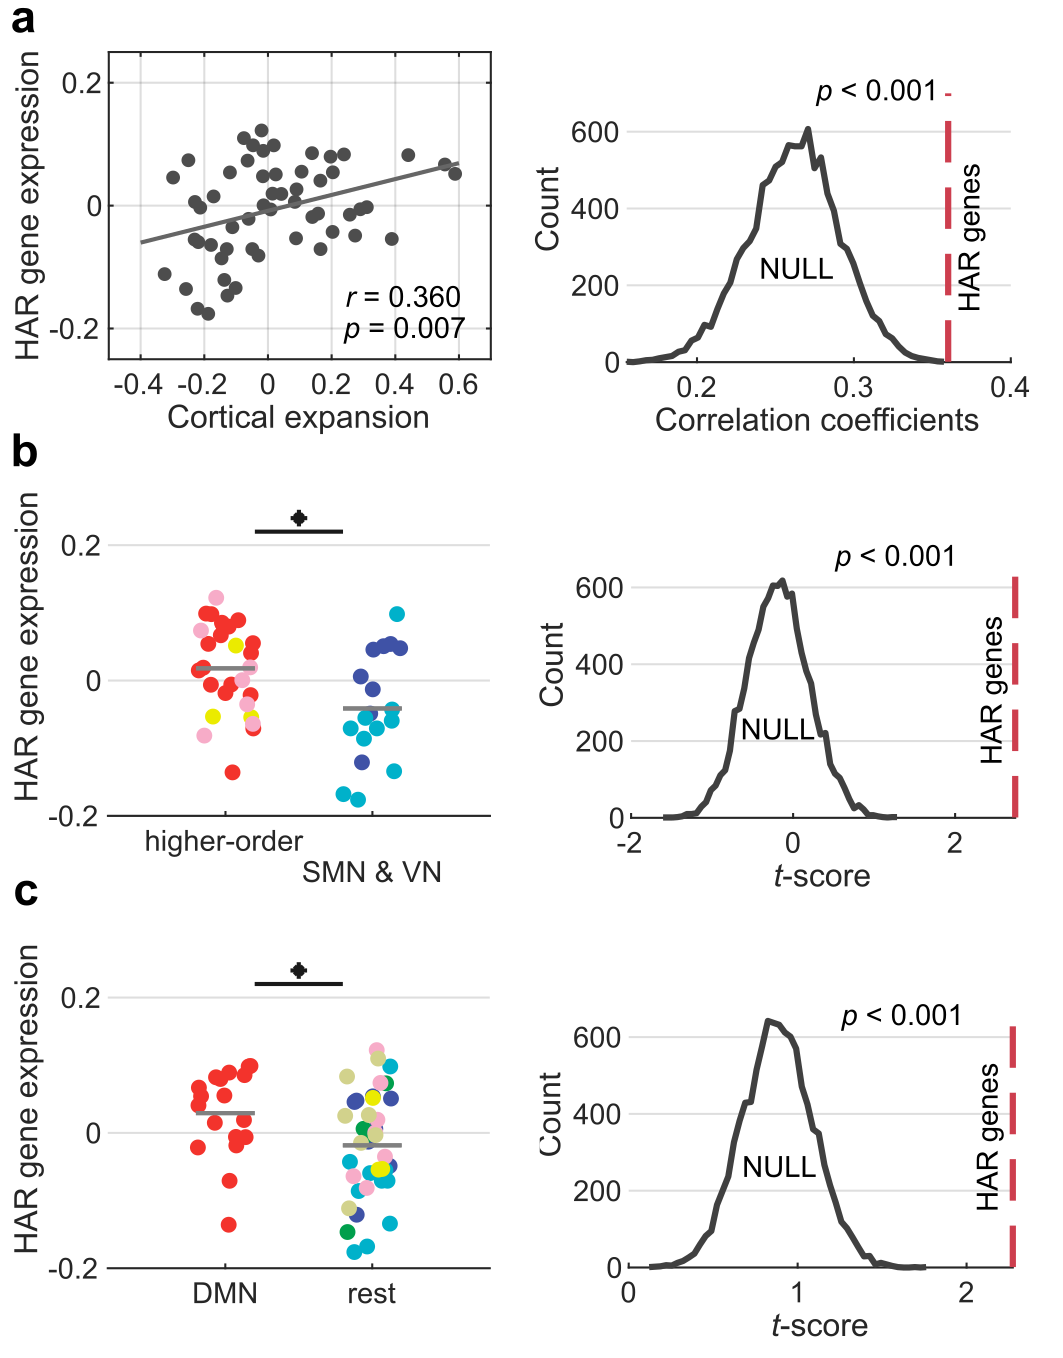
\includegraphics[width=10cm]{images/harFigS1.png}
    \caption{HAR gene expression. (a) Cortical HAR gene expression is significantly correlated with the normalized chimpanzee-human cortical expansion (\rvaldf(53) = 0.360, \pval = 0.007) (left), with the effect significantly exceeding the null condition generated by ECE genes (\pval < 0.001, 10,000 permutations) (right). (b) Cortical HAR gene expression in regions of higher-order networks is significantly higher than regions of the SMN/VN (\tvaldf(55) = 2.742, \pval = 0.009) (left), with the effect above the null condition generated by ECE genes (\pval < 0.001, 10,000 permutations) (right). (c) Cortical HAR gene expression in regions of DMN is marginally higher than the rest of the cortex (\tvaldf(55) = 2.274, \pval = 0.027, uncorrected) (left), also, with the effect significantly exceeding the null condition generated by ECE genes (\pval < 0.001, 10,000 permutations) (right). Colors indicate functional networks, as in Figure \ref{harFig2} in the main text.}
    \label{harFigs1}
\end{figure}


\begin{figure}[H]
    \centering
    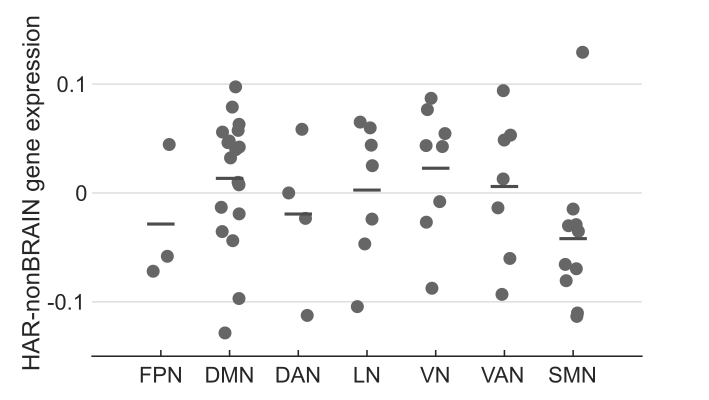
\includegraphics[width=8cm]{images/harFigS2.png}
    \caption{HAR-nonBRAIN gene expression. HAR-nonBRAIN gene expression within each of the seven functional networks, ranked in descending order according to their mean expansion per net-work (as in Figure \ref{harFig2}c).}
    \label{harFigs2}
\end{figure}

\begin{figure}[H]
    \centering
    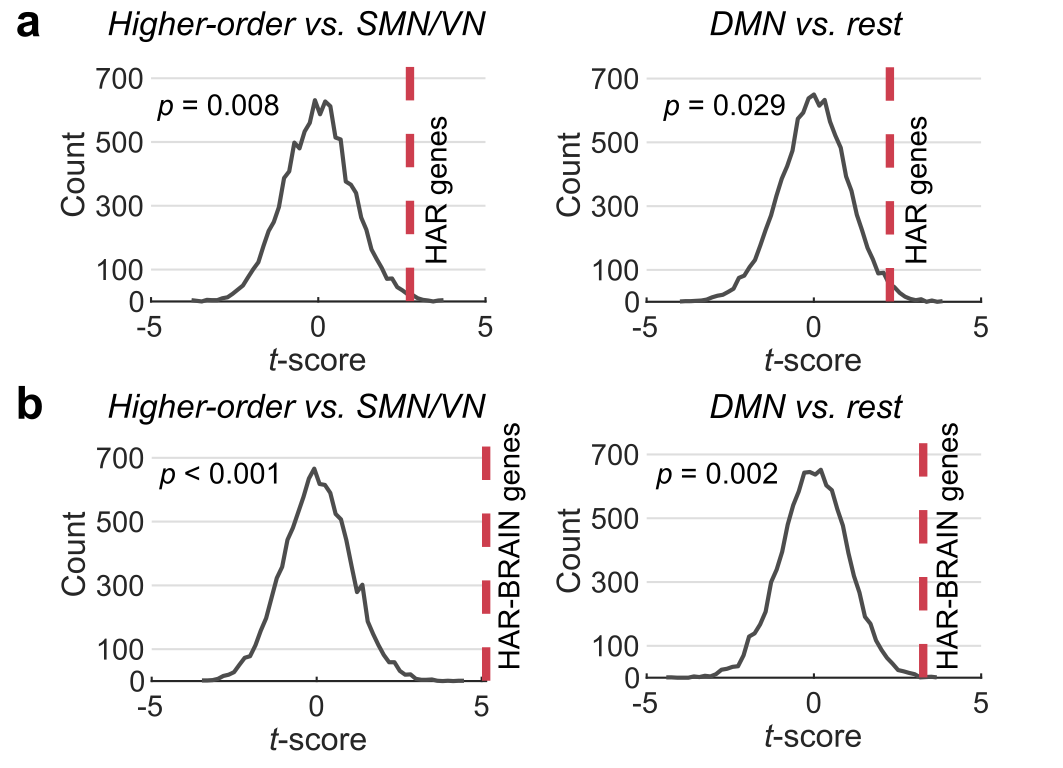
\includegraphics[width=10cm]{images/harFigS3.png}
    \caption{Permutation testing of HAR/HAR-BRAIN gene expression by randomly shuffling cortical regions. (a) HAR gene expression between higher-order networks and the SMN/VN (left panel) and between the DMN and the rest of the cortex (right panel). (b) HAR-BRAIN gene expres-sion between higher-order networks and the SMN/VN (left panel) and between the DMN and the rest of the cortex (right panel).}
    \label{harFigs3}
\end{figure}

\begin{figure}[H]
    \centering
    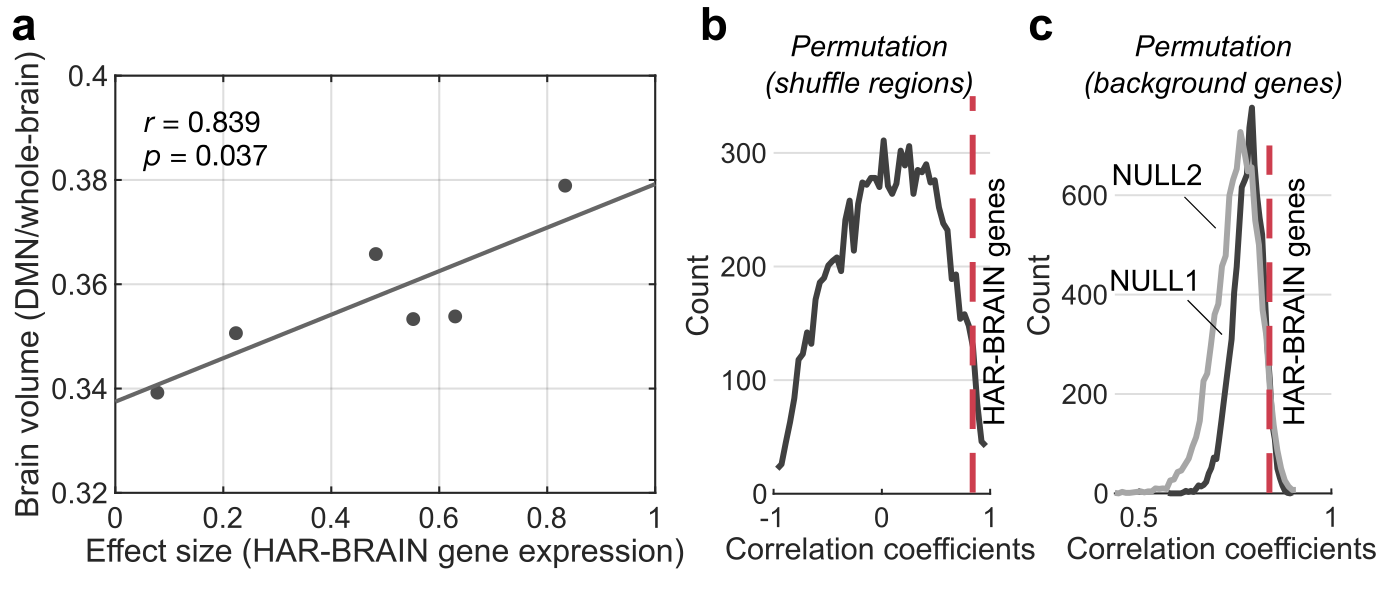
\includegraphics[width=12cm]{images/harFigS4.png}
    \caption{HAR-BRAIN gene expression and cortical volume. (a) Effect size of HAR-BRAIN gene expression difference between the DMN and the rest of the cortex significantly correlates to the ratio of brain volume of the DMN regions (\rval = 0.839, \pval = 0.037). Brain volume is calculated by running FreeSurfer on the ex-vivo T1-weighted MRI of each brain donor (downloaded from \url{https://human.brain-map.org/mri\_viewers/data}). (b) The correlation coefficient in (a) significantly exceeds the null distribution of correlation coefficients generated by randomly shuffling brain regions (two-sided \pval = 0.047, 10,000 permutations). (c) The correlation coefficient in (a) does not significantly exceed the null distribution of correlation coefficients generated by randomly selecting background genes, with only trend-level effects observed for BRAIN genes (NULL1, \pval = 0.095, n.s.) and ECE genes (NULL2, \pval = 0.090, n.s., 10,000 permutations).}
    \label{harFigs4}
\end{figure}

\begin{figure}[H]
    \centering
    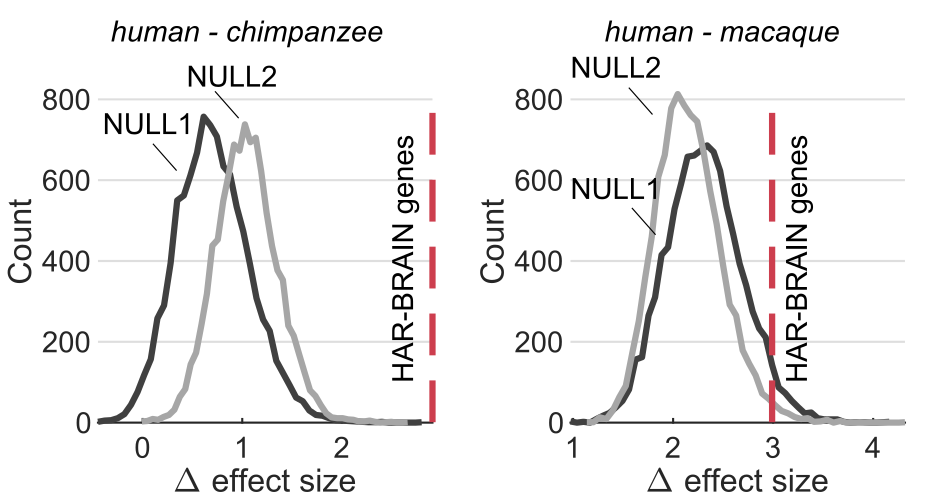
\includegraphics[width=10cm]{images/harFigS5.png}
    \caption{HAR-BRAIN gene expression enhancement in cognitive network regions in humans compared to chimpanzees/macaques. Left: permutation testing shows the Δ effect size of the enhanced HAR-BRAIN gene expression in cognitive network regions between humans and chimpanzees to significantly exceed null distributions of Δ effect size computed by randomly selecting gene sets from the pool of BRAIN genes (NULL1: \pval < 0.001) and evolutionarily conserved genes (ECE genes; NULL2: \pval < 0.001, 10,000 permutations). Right: permutation testing shows the Δ effect size of the enhanced HAR-BRAIN gene expression in cognitive network regions between humans and macaques to significantly exceed NULL2 (two-sided \pval = 0.026), but not NULL1 (two-sided \pval = 0.090, 10,000 permutations). The marginal trend-level effect found for NULL1 might be due to the notion of macaques and humans to be more genetically different as compared to chimpanzees, and the set of HAR-BRAIN genes thus to only partially cover the evolutionarily genetic differentiations between the human and macaque and many genetically differences to remain in the NULL condition.}
    \label{harFigs5}
\end{figure}

\begin{figure}[H]
    \centering
    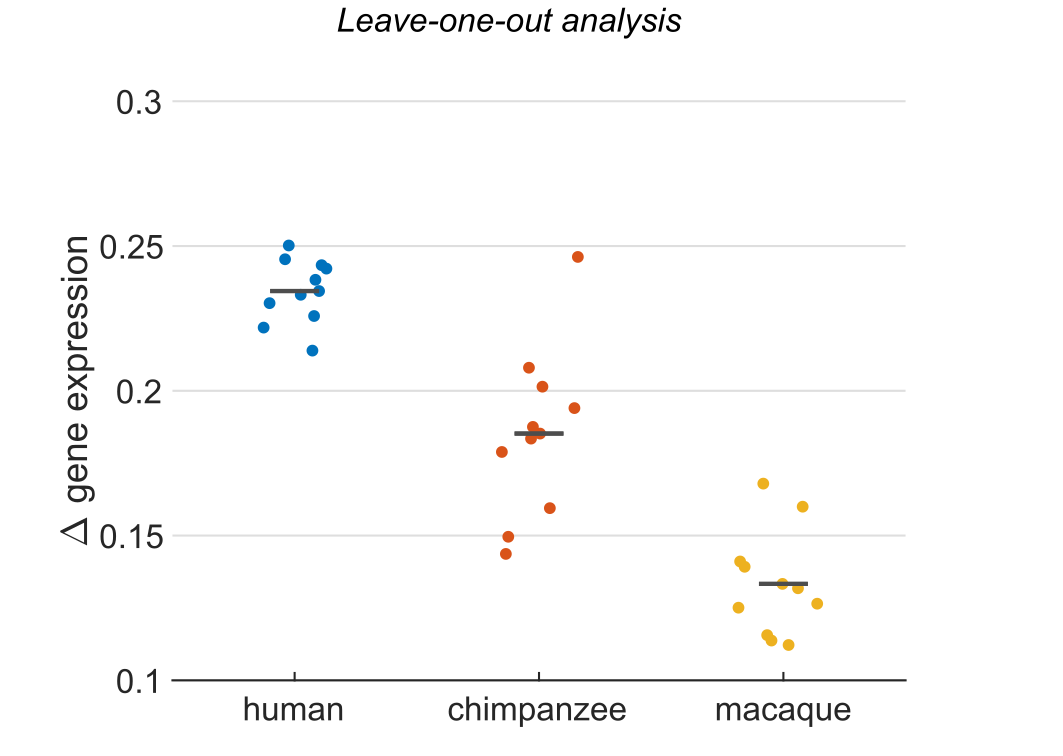
\includegraphics[width=8cm]{images/harFigS6.png}
    \caption{Leave-one-out analysis by computing the difference of mean gene expression (Δ gene expression) between cognitive network regions and primary regions for ten rounds, in each of which one region out of the ten regions was excluded. The resulting Δ gene expression in humans is larger than that in chimpanzees in 9/10 rounds and that in macaques in all 10 rounds.}
    \label{harFigs6}
\end{figure}

\begin{figure}[H]
    \centering
    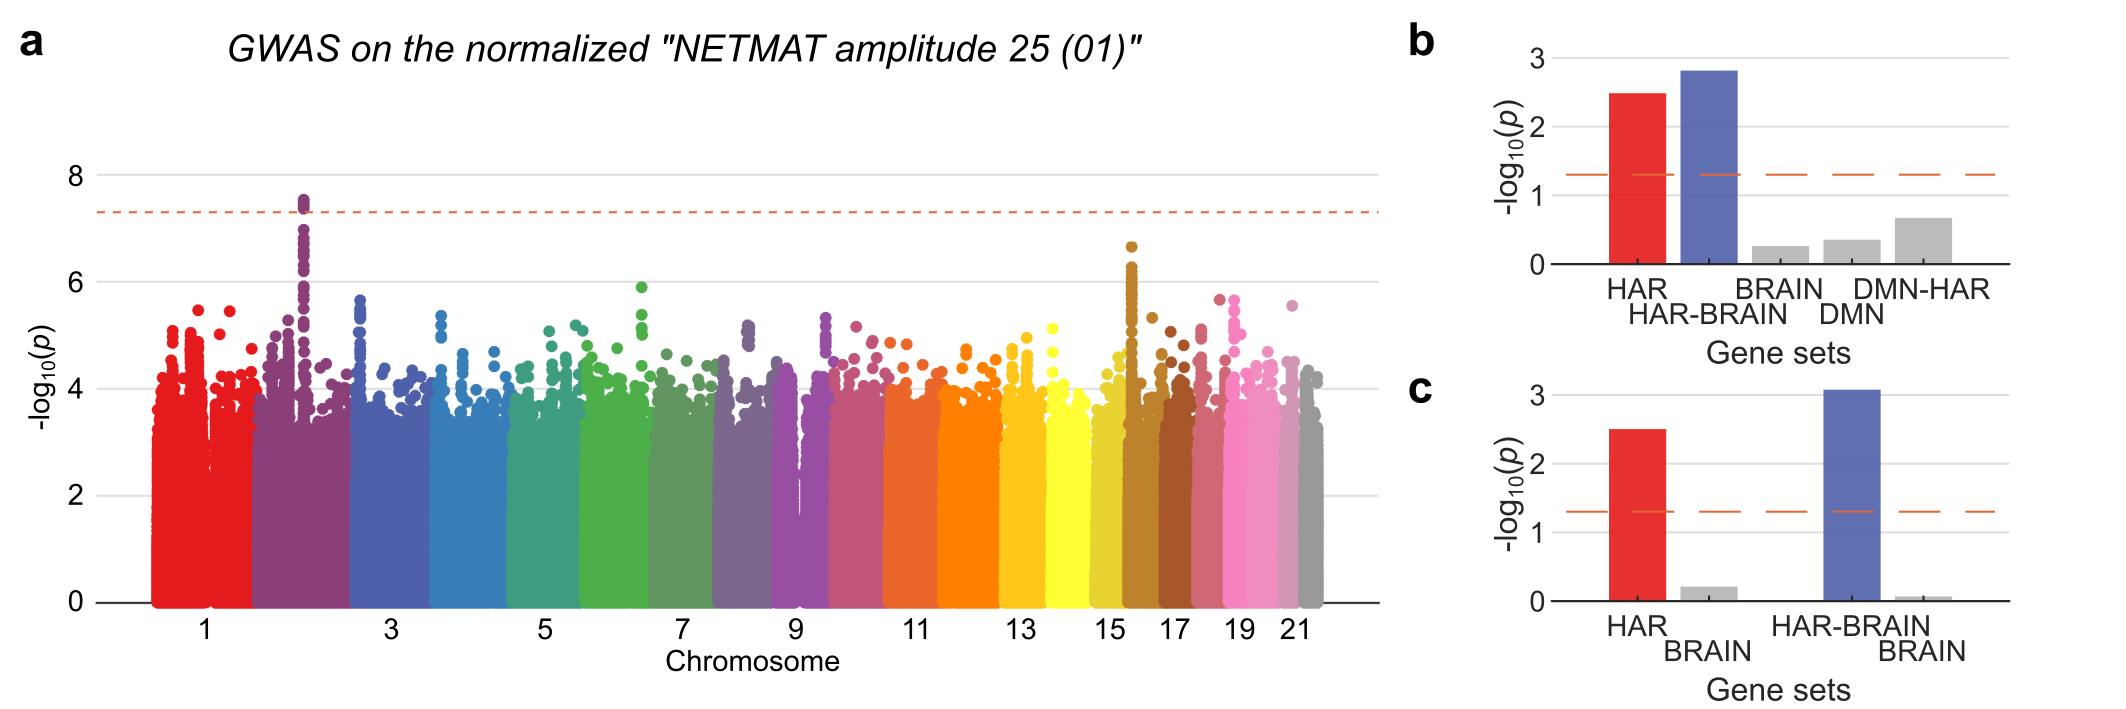
\includegraphics[width=\linewidth]{images/harFigS7.png}
    \caption{GWAS on the normalized DMN functional activity. (a) Manhattan plot showing -log10-transformed two-tailed p value of each SNP from the GWAS analysis on the y axis and base-pair positions along the chromosomes on the x axis. Dotted red line indicates Bonferroni-corrected genome-wide significance (\pval < 5 × 10\textsuperscript{-8}). (b) MAGMA gene-set analysis. -log10-transformed \textit{p}-values of the associations between HAR, HAR-BRAIN, BRAIN, DMN, and DMN-HAR genes and DMN functional activity are displayed. Dashed line indicates \pval = 0.05. (c) MAGMA conditional gene-set analysis. -log10-transformed \textit{p}-values of the associations be-tween HAR and HAR-BRAIN genes and DMN functional activity are displayed, with BRAIN genes taken as covariant. Dashed line indicates \pval = 0.05.}
    \label{harFigs7}
\end{figure}

\begin{figure}[H]
    \centering
    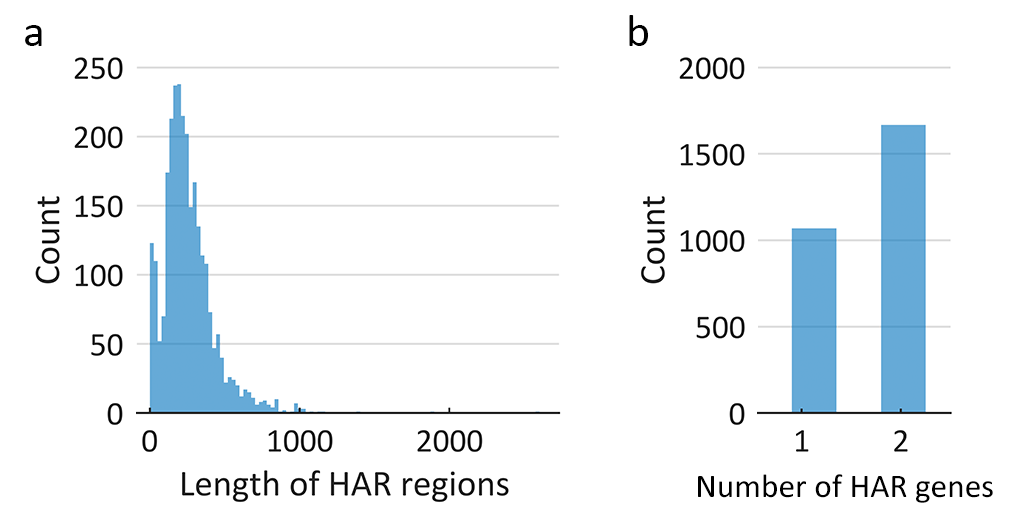
\includegraphics[width=10cm]{images/harFigS8.png}
    \caption{Distributions of lengths of the HAR regions (a) and the number of genes mapped from each HAR region (b).}
    \label{harFigs8}
\end{figure}

\begin{figure}[H]
    \centering
    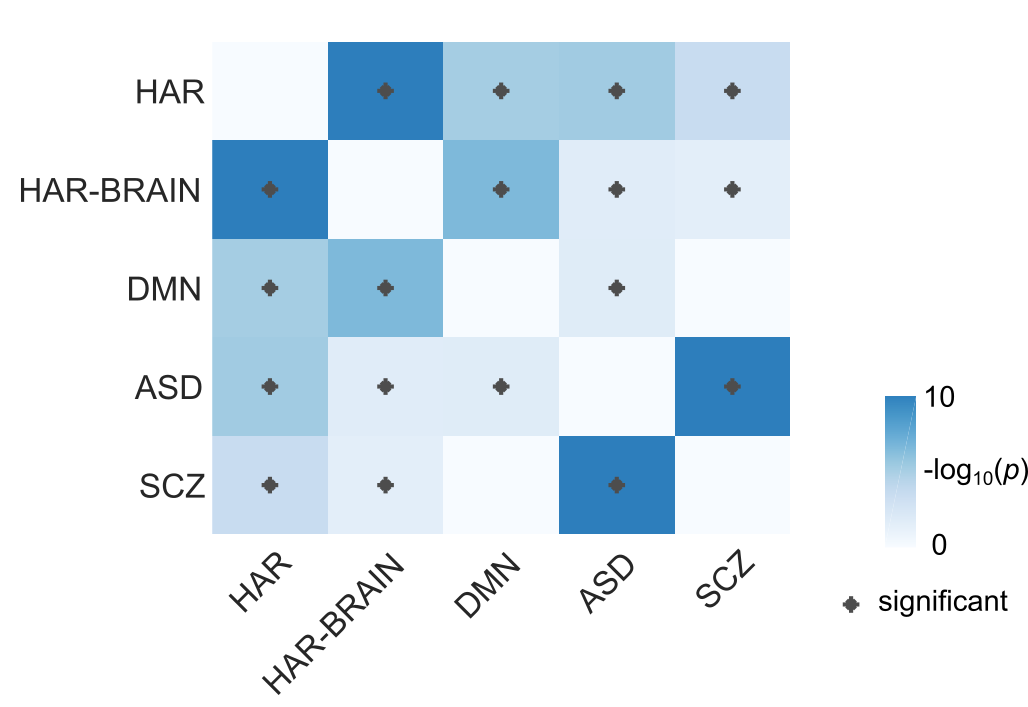
\includegraphics[width=8cm]{images/harFigS9.png}
    \caption{Enrichment of HAR, HAR-BRAIN, and DMN genes in rare variations of ASD and schizophrenia (SCZ). \textit{p}-values obtained from hypergeometric test.}
    \label{harFigs9}
\end{figure}

\begin{figure}[H]
    \centering
    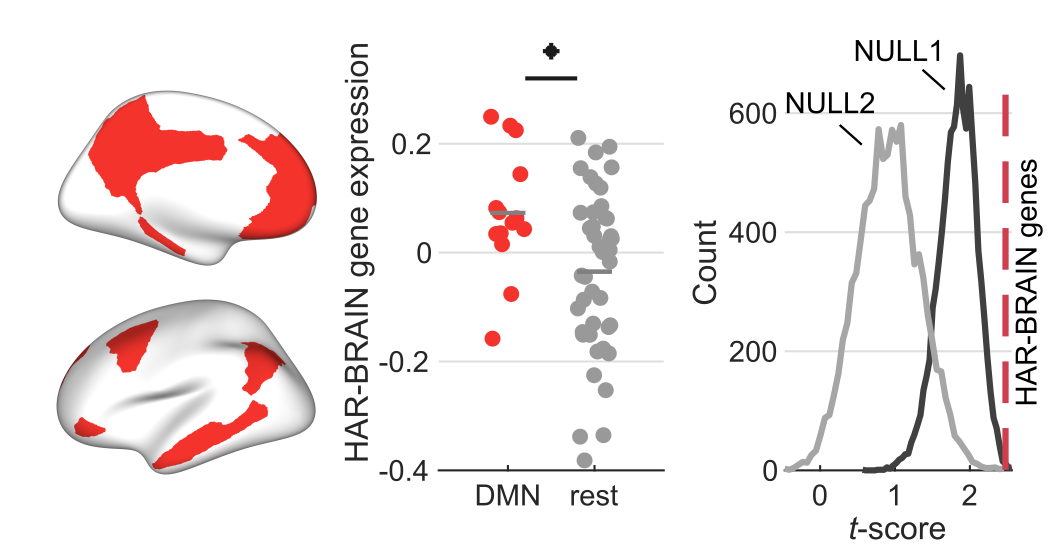
\includegraphics[width=10cm]{images/harFigS10.png}
    \caption{DMN assignment adapted from Raichle (2015) \citep{raichle2015brain}. Using the DMN assignment adapted from Raichle (2015) (left panel), DMN regions consistently show higher gene expression of HAR-BRAIN genes compared to the rest of the cortex (\tvaldf(55) = 2.476, \pval = 0.016) (middle panel), with the \textit{t}-score significantly exceeding null distributions generated by random BRAIN genes (NULL1, \pval = 0.003) and ECE genes (NULL2, \pval < 0.001) (right panel).}
    \label{harFigs10}
\end{figure}

\begin{figure}[H]
    \centering
    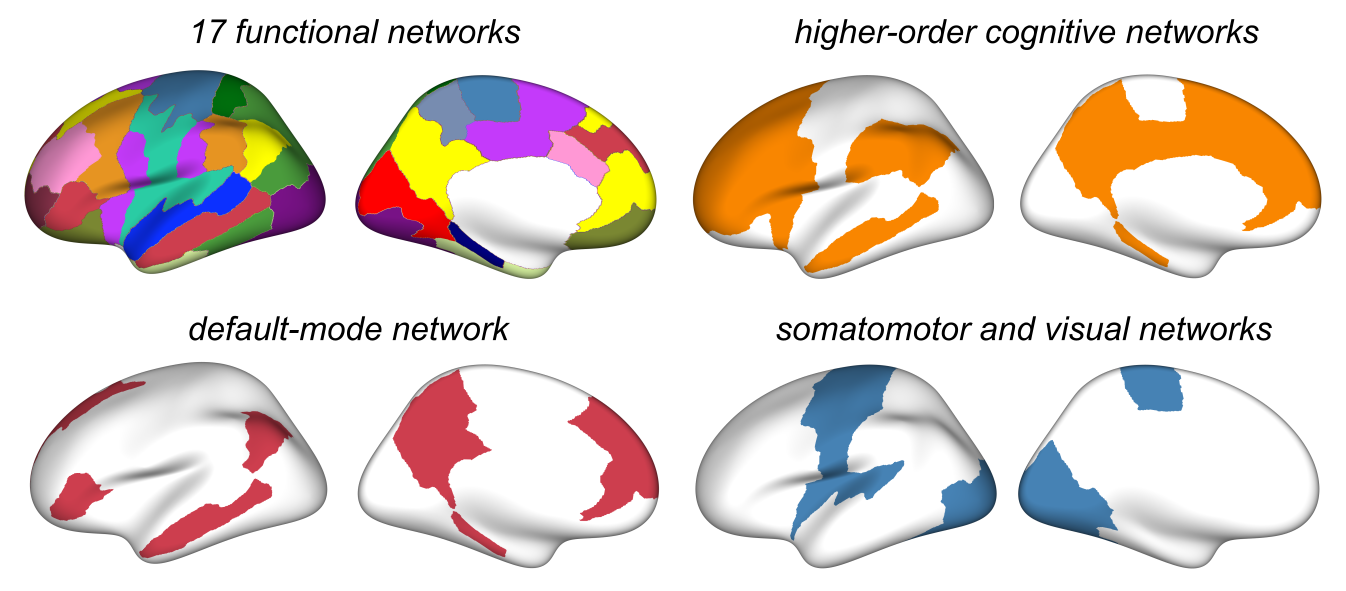
\includegraphics[width=10cm]{images/harFigS11.png}
    \caption{Seventeen functional networks. DK cortical regions were assigned to 17 functional networks for validation (top left panel). Networks labeled as 11, 15, 16, and 17 were grouped into the default-mode network (bottom left panel). Grouping the default-mode network and networks labeled as 7, 8, 12, and 13 formed the higher-order cognitive networks (top right panel). Networks labeled as 1, 2, 3, and 4 were defined as primary networks (bottom right panel).}
    \label{harFigs11}
\end{figure}

\begin{figure}[H]
    \centering
    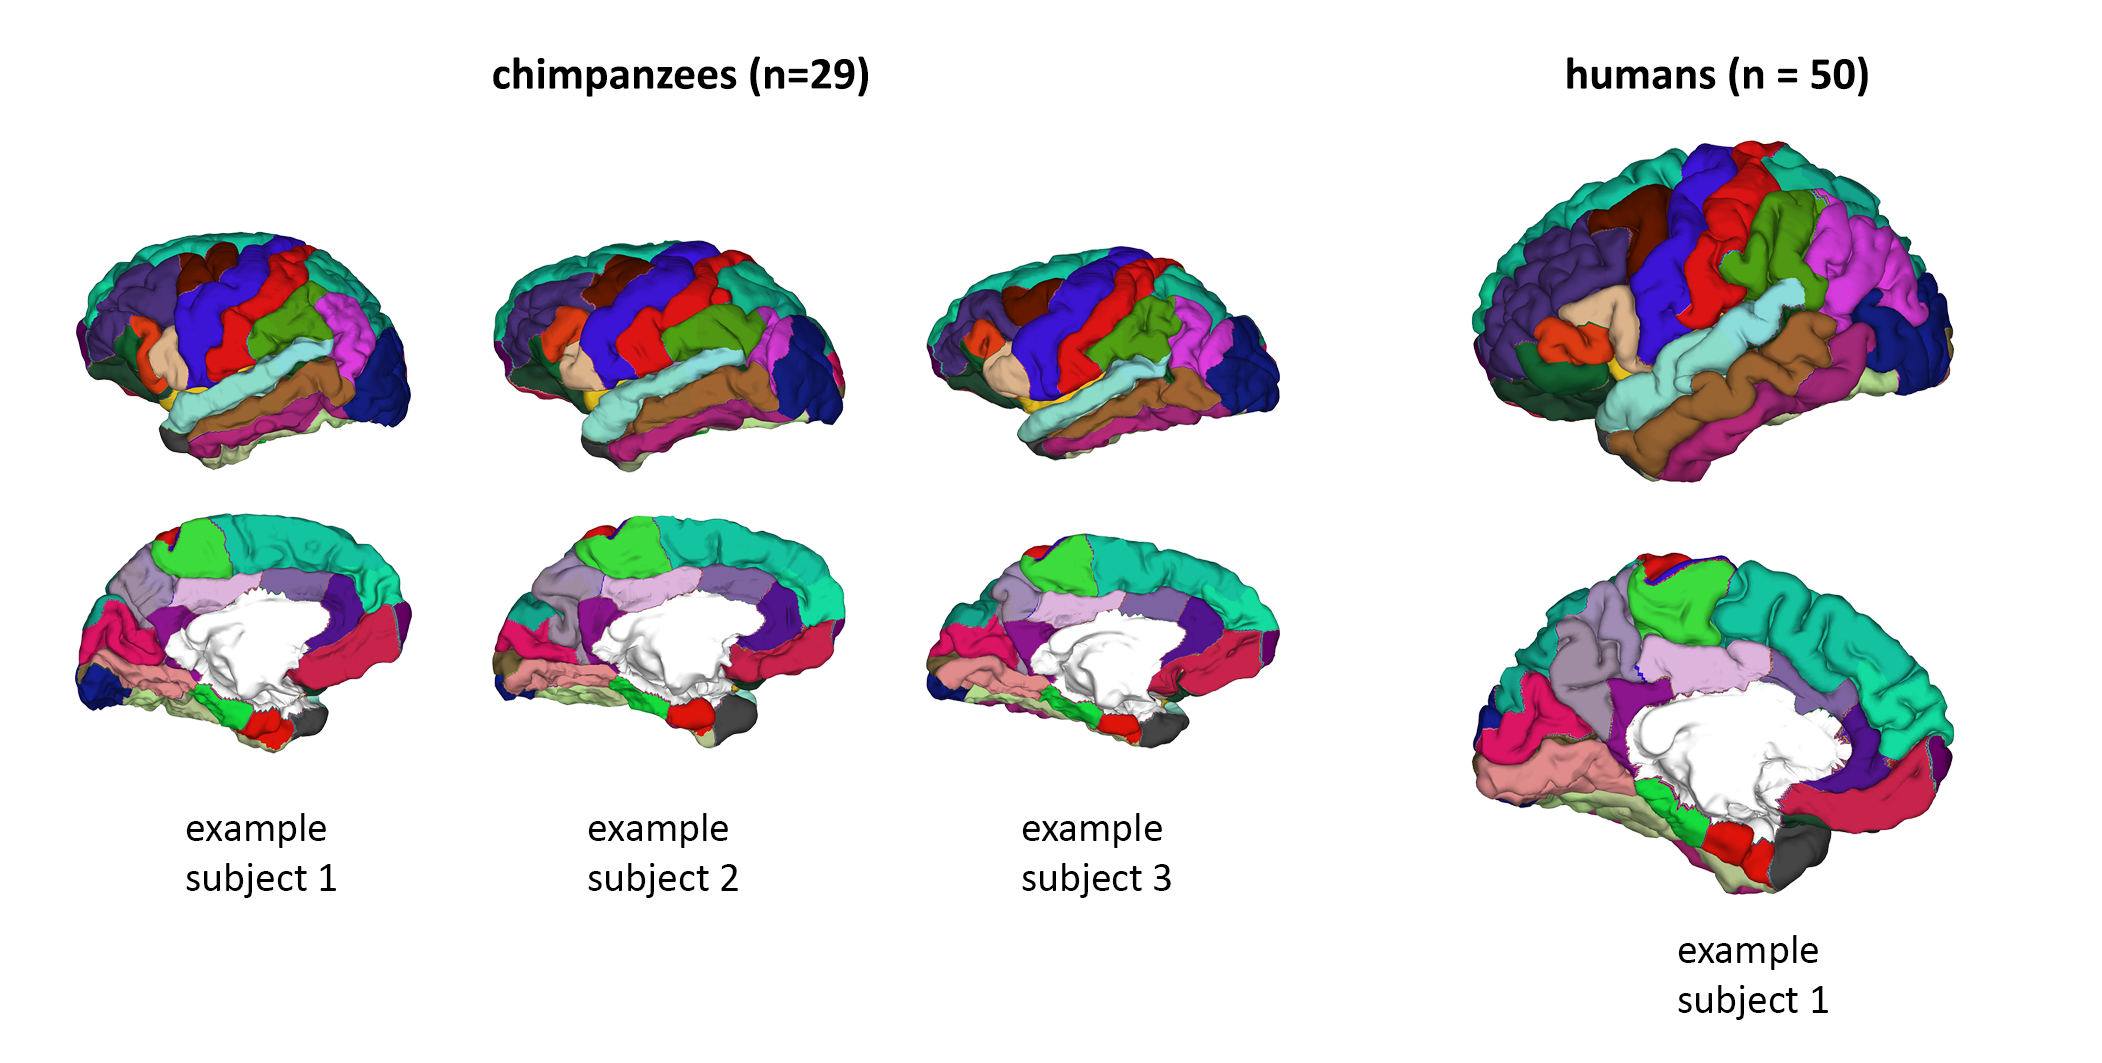
\includegraphics[width=\linewidth]{images/harFigS12.png}
    \caption{Example cortical parcellations of chimpanzees and humans.}
    \label{harFigs12}
\end{figure}

\begin{figure}[H]
    \centering
    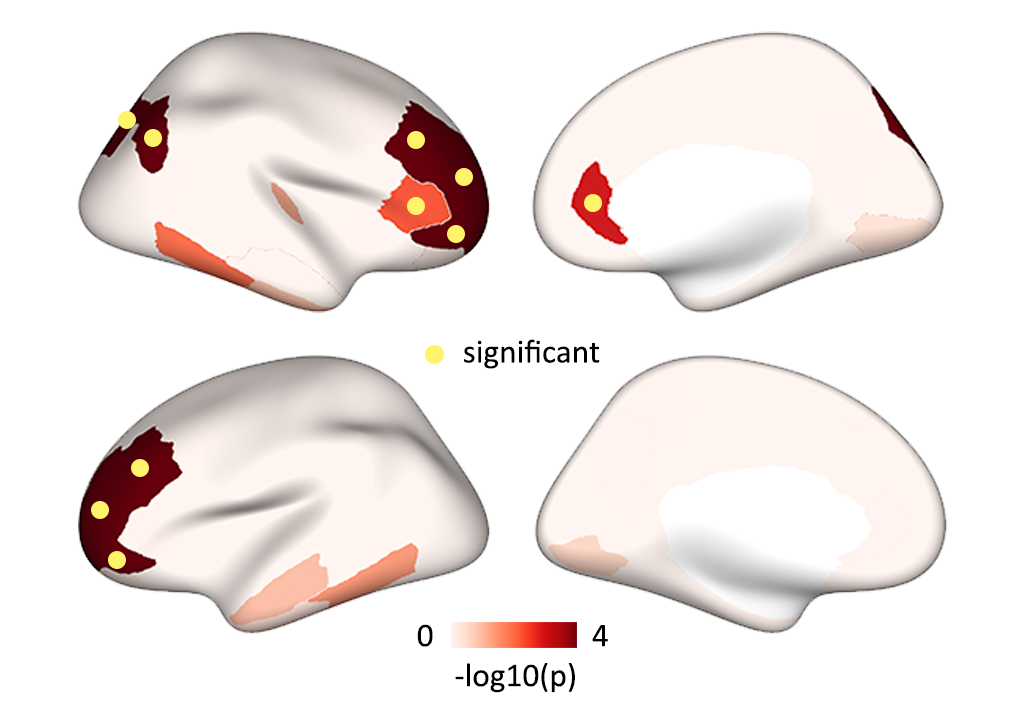
\includegraphics[width=8cm]{images/harFigS13.png}
    \caption{Brain maps of regions showing significant chimpanzee-to-human expansion in permutation testing based on region shuffling. \textit{p}-values obtained from 10,000 permutations.}
    \label{harFigs13}
\end{figure}

\begin{figure}[H]
    \centering
    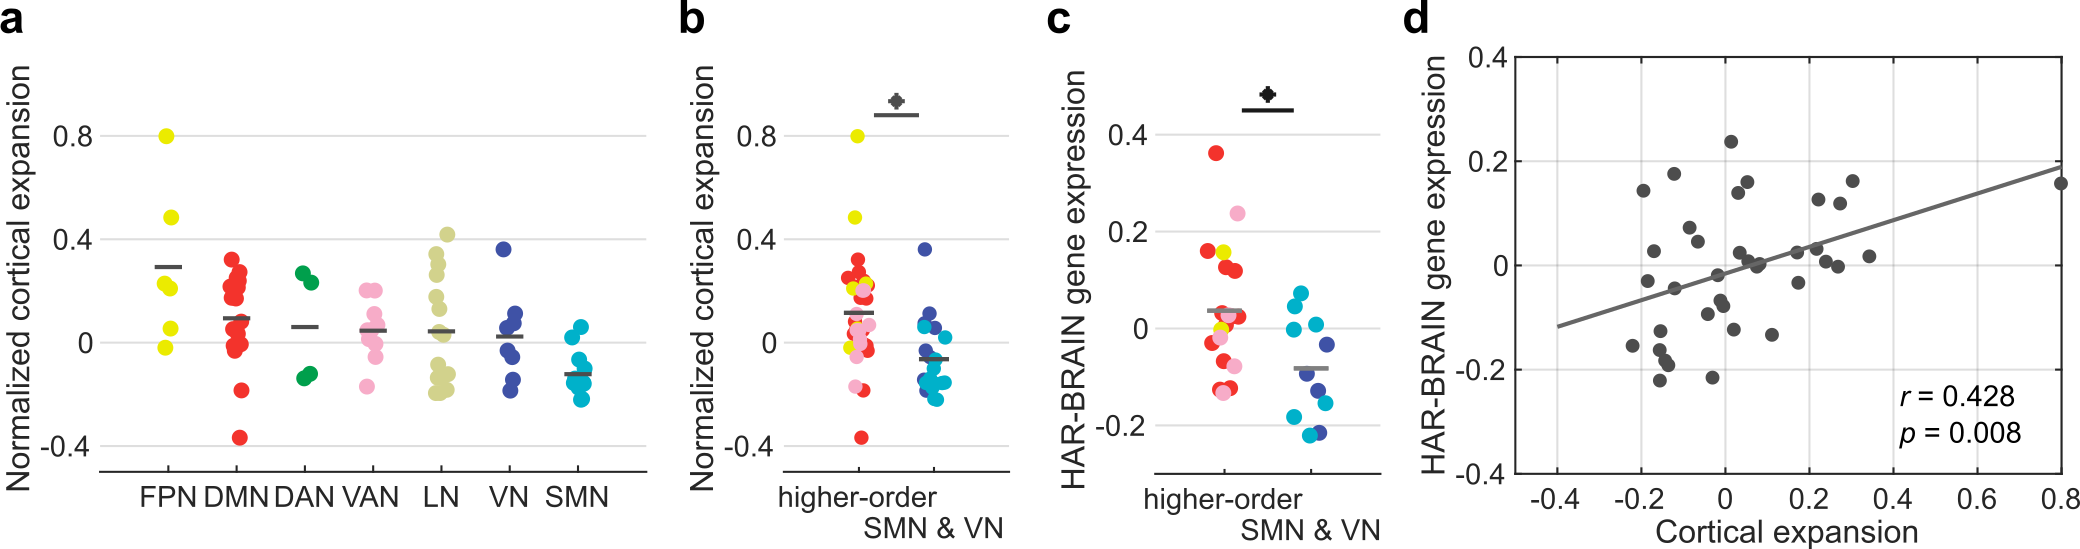
\includegraphics[width=\linewidth]{images/harFigS14.png}
    \caption{Evolutionary cortical expansion and HAR-BRAIN gene expression in BB-38 chimpanzee-human atlas. (a) Levels of the cortical expansion per functional network in descending order. VN: visual network, SMN: somatomotor network, DAN: dorsal-attention network, LN: limbic network, VAN: ventral-attention network, FPN: frontal parietal network, DMN: default-mode network. (b) Regions of higher-order cognitive networks (DMN, FPN, VAN), present signifi-cant larger expansion compared to regions in SMN and VN (\tvaldf(28) = 3.632, \pval < 0.001). (c) Regions of higher-order cognitive networks (DMN, FPN, VAN), show significantly higher HAR-BRAIN expression compared to regions in SMN and VN (\tvaldf(28) = 2.572, \pval = 0.016). (d) Cortical expansion significantly correlates to cortical HAR-BRAIN gene expression (\rval = 0.428, \pval = 0.008).}
    \label{harFigs14}
\end{figure}

\newpage
\subsection*{Supplementary References}
\printbibliography[heading=none]

\end{refsection}

